\documentclass[10pt]{article}
\usepackage[export]{adjustbox}
\usepackage{amsmath}
\usepackage[makeroom]{cancel}
\usepackage{enumitem}
\usepackage{graphicx}
%Load mhchem using some package options
\usepackage[version=4]{mhchem}
\usepackage{multicol}
\usepackage{siunitx}

\title{
    Problem Set \#3
    \\  \small
    CHEM101A: General College Chemistry
    }
\author{Donald Aingworth IV}
\date{September 5, 2025}

\begin{document}
    \DeclareSIUnit{\molarity}{M}
    \DeclareSIUnit{\M}{M}

    \maketitle

    \pagebreak
    \section{Topic B Problem 13}
        For each of the mixtures below, do the following:

        \noindent
        1) Identify the actual species that are present in the mixture (before any reaction occurs).
        
        \noindent
        2) Write the formula of any product that forms. If no product will form, write “no reaction” and skip Step 3.
        
        \noindent
        3) Write the net ionic equation for the reaction that occurs, including the state of each
        substance (s, l, g, or aq).

        \textit{
            Example: Mixing 0.1 M \ce{NaCl} and 0.1 M \ce{Pb(NO3)2}
            (a) The actual species are \ce{Na+}, \ce{Cl-}, \ce{Pb^2+}, and \ce{NO3-}
            (b) \ce{PbCl2} will form (because it is insoluble in water)
            (c) The net ionic equation is \ce{Pb^2+ (aq) + 2 Cl- (aq) -> PbCl2 (s)}
            }
        
        a) Mixing 0.1 M \ce{MgCl2} and 0.1 M \ce{Na3PO4}
    
        b) Mixing 0.1 M \ce{HNO3} and 0.1 M \ce{NaOH}
    
        c) Mixing 0.1 M \ce{Fe(NO3)3} and 0.1 M \ce{KOH}
    
        d) Mixing 0.1 M \ce{ZnBr2} and 0.1 M \ce{CuSO4}
    
        e) Mixing 0.1 M \ce{HCl} and 0.1 M \ce{NaHCO3}
    
        f) Mixing 0.1 M \ce{AgNO3} and 0.1 M \ce{K2CO3}
    
        g) Mixing 0.1 M \ce{Ba(OH)2} and 0.1 M \ce{Na2SO4}
    
        h) Mixing 0.1 M \ce{HC2H3O2} and 0.1 M \ce{Ba(OH)2}
    
        i) Mixing 0.1 M \ce{HC6H5O} and 0.1 M \ce{NaOH}
    
        j) Mixing 0.1 M \ce{H2C4H4O4} (succinic acid) and excess 0.1 M \ce{NaOH}. (Hint: You should write two equations for this.)


        \subsection{Solution}
            \begin{center}
                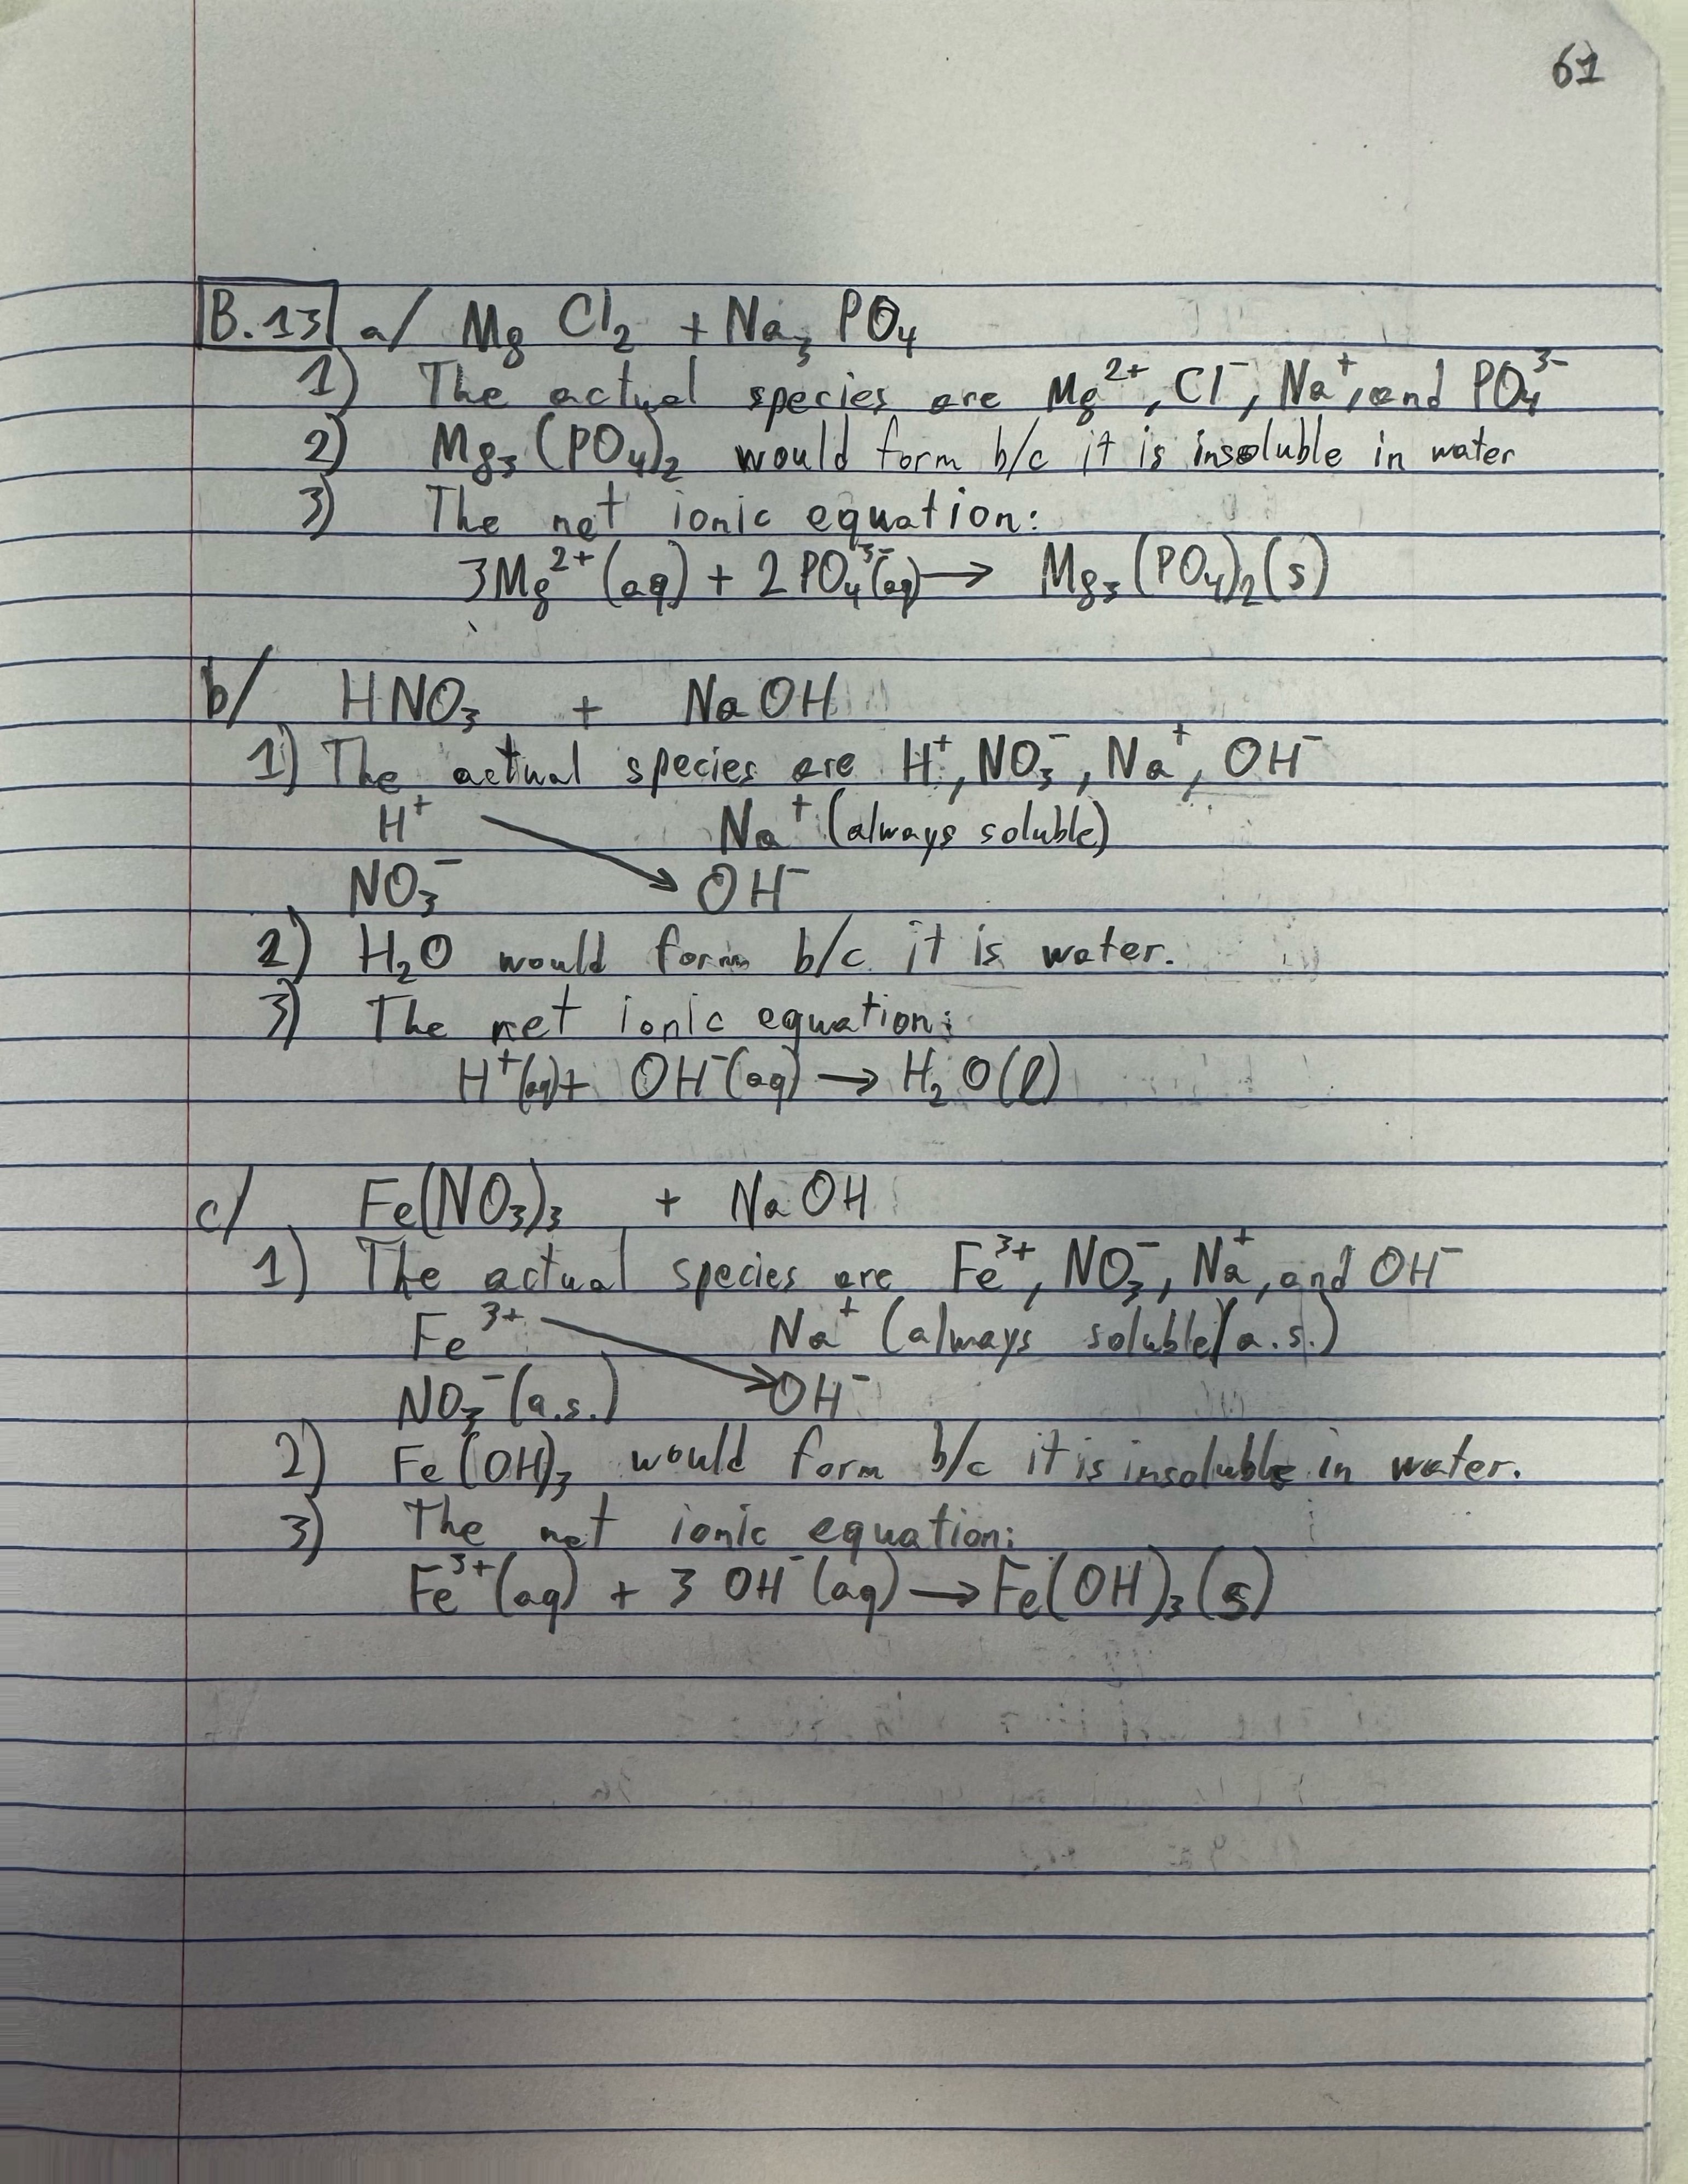
\includegraphics[width=\textwidth, trim={5in 27in 3in 6in},clip]{"Answers Images/IMG_6647.jpg"}

                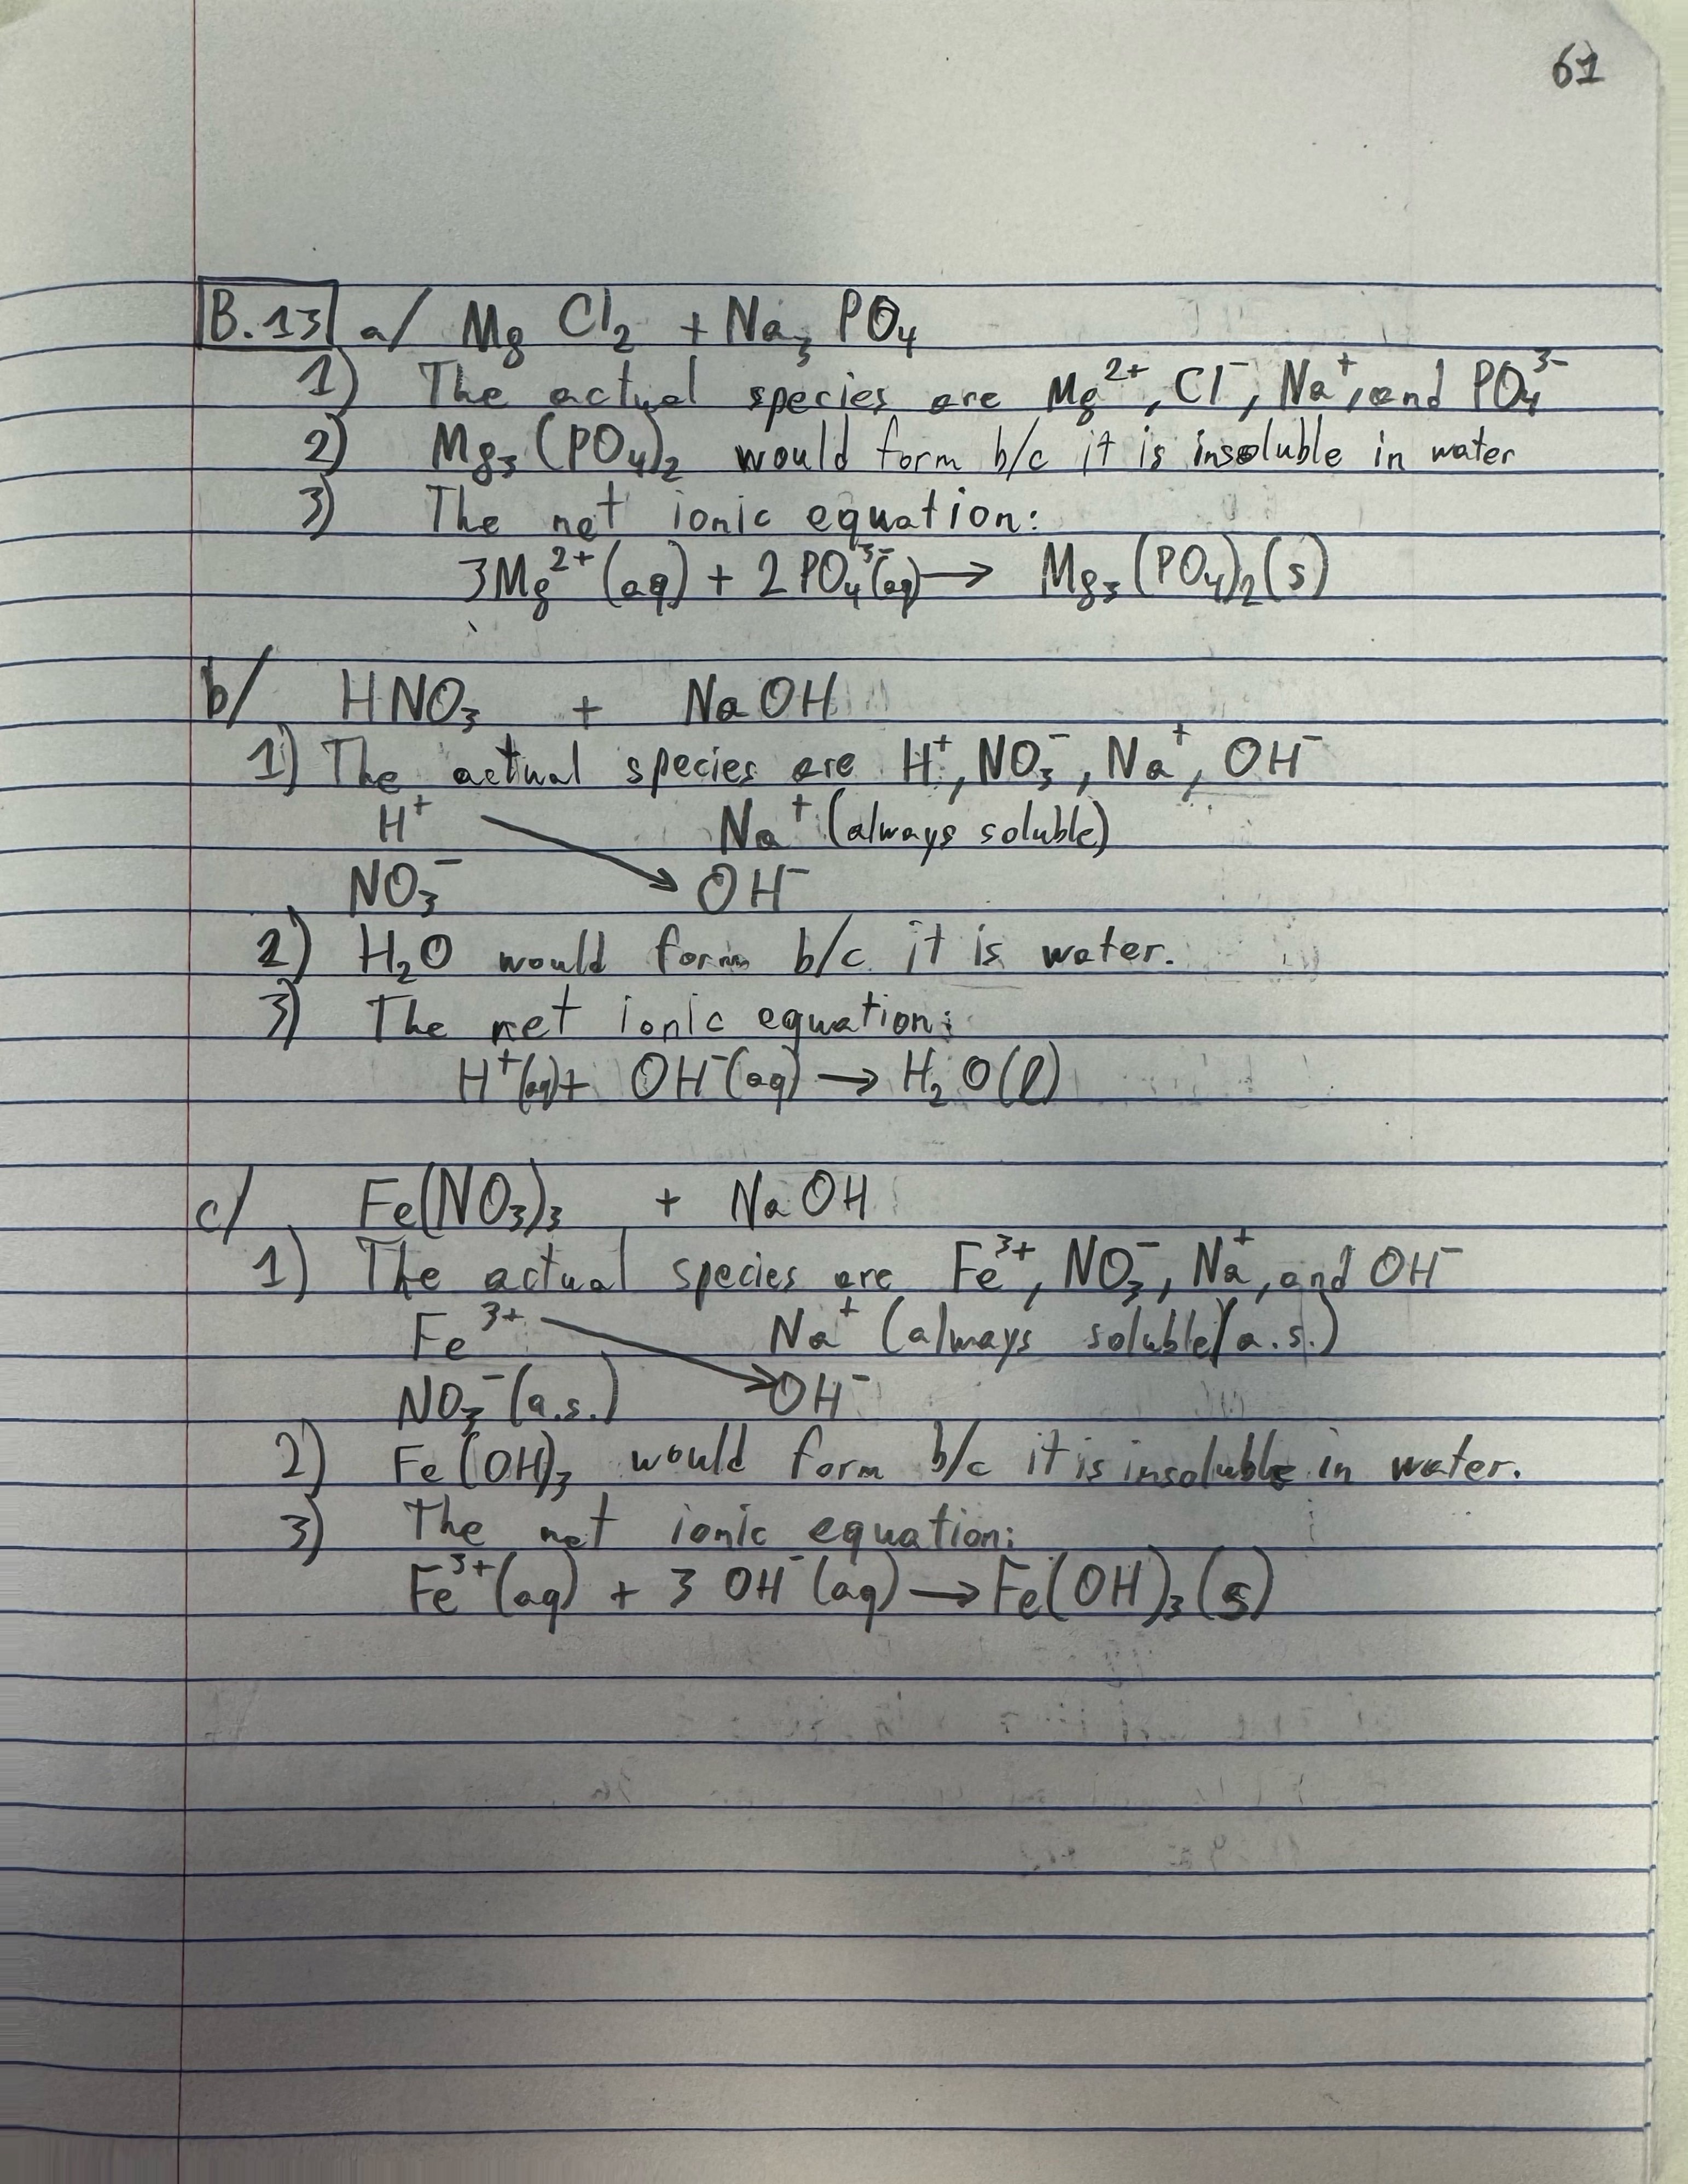
\includegraphics[width=\textwidth, trim={5in 13.5in 3in 29in},clip]{"Answers Images/IMG_6647.jpg"}

                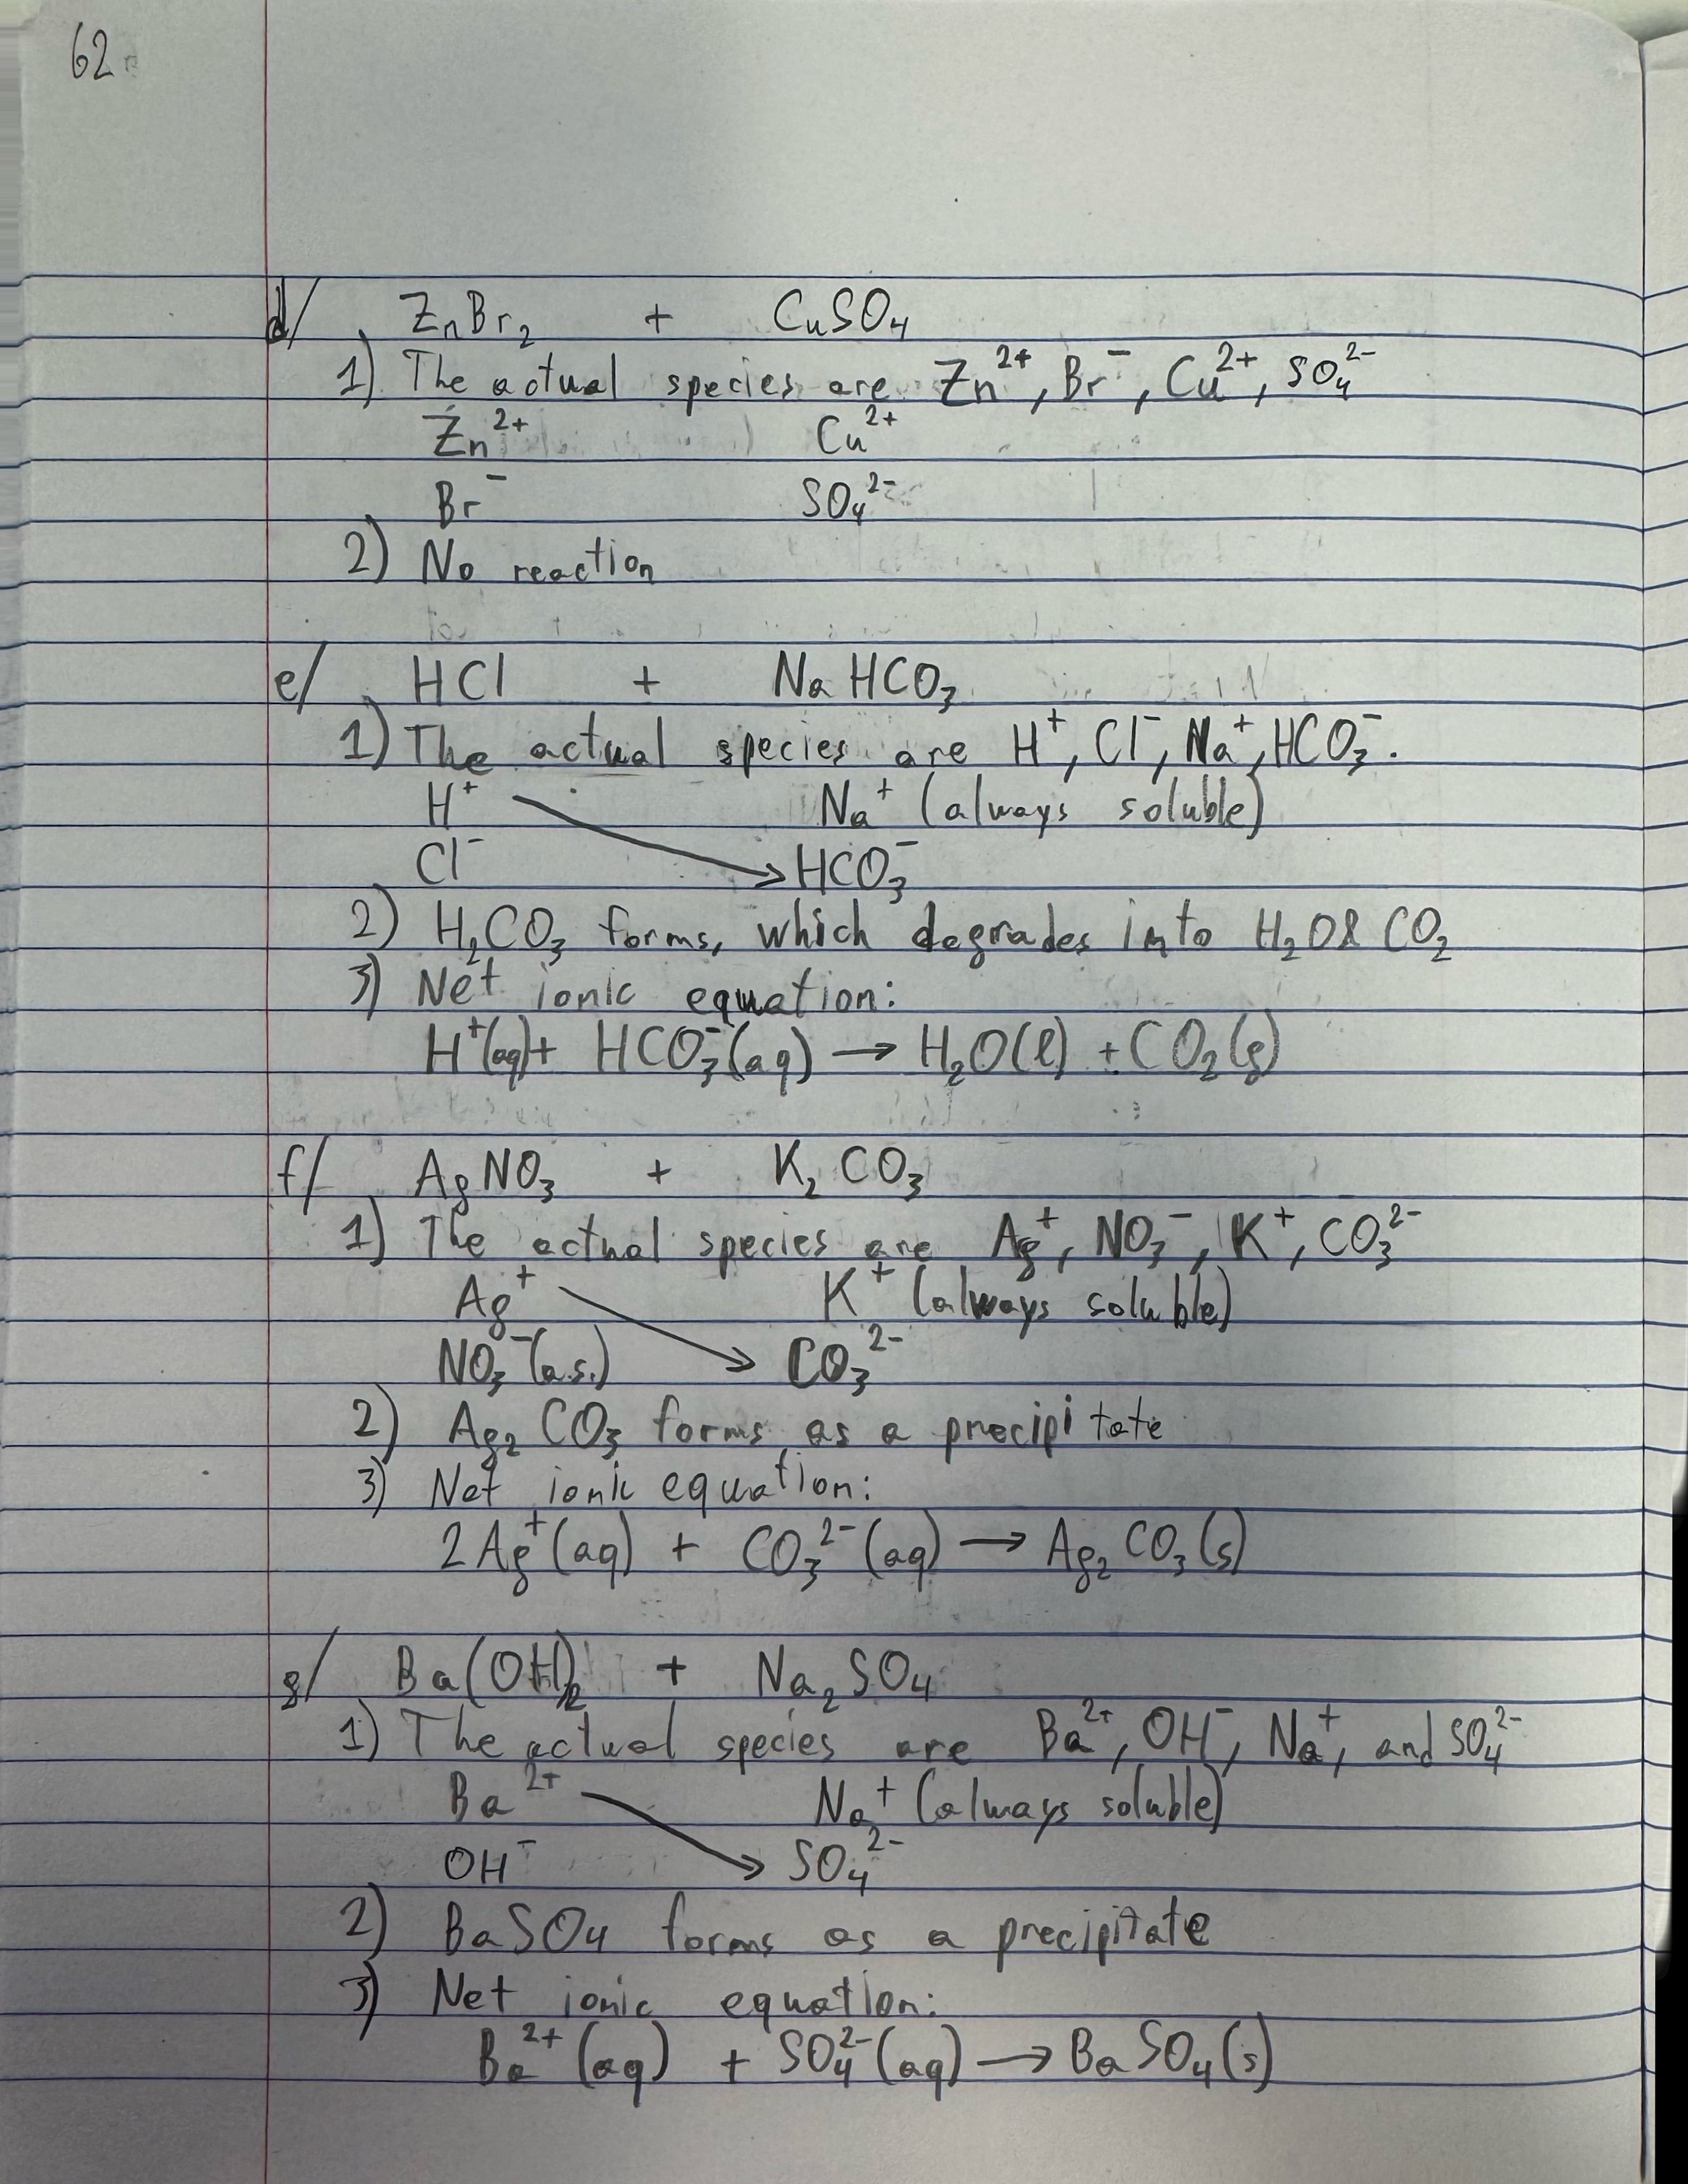
\includegraphics[width=\textwidth, trim={5in 13.5in 3in 5in},clip]{"Answers Images/IMG_6648.jpg"}

                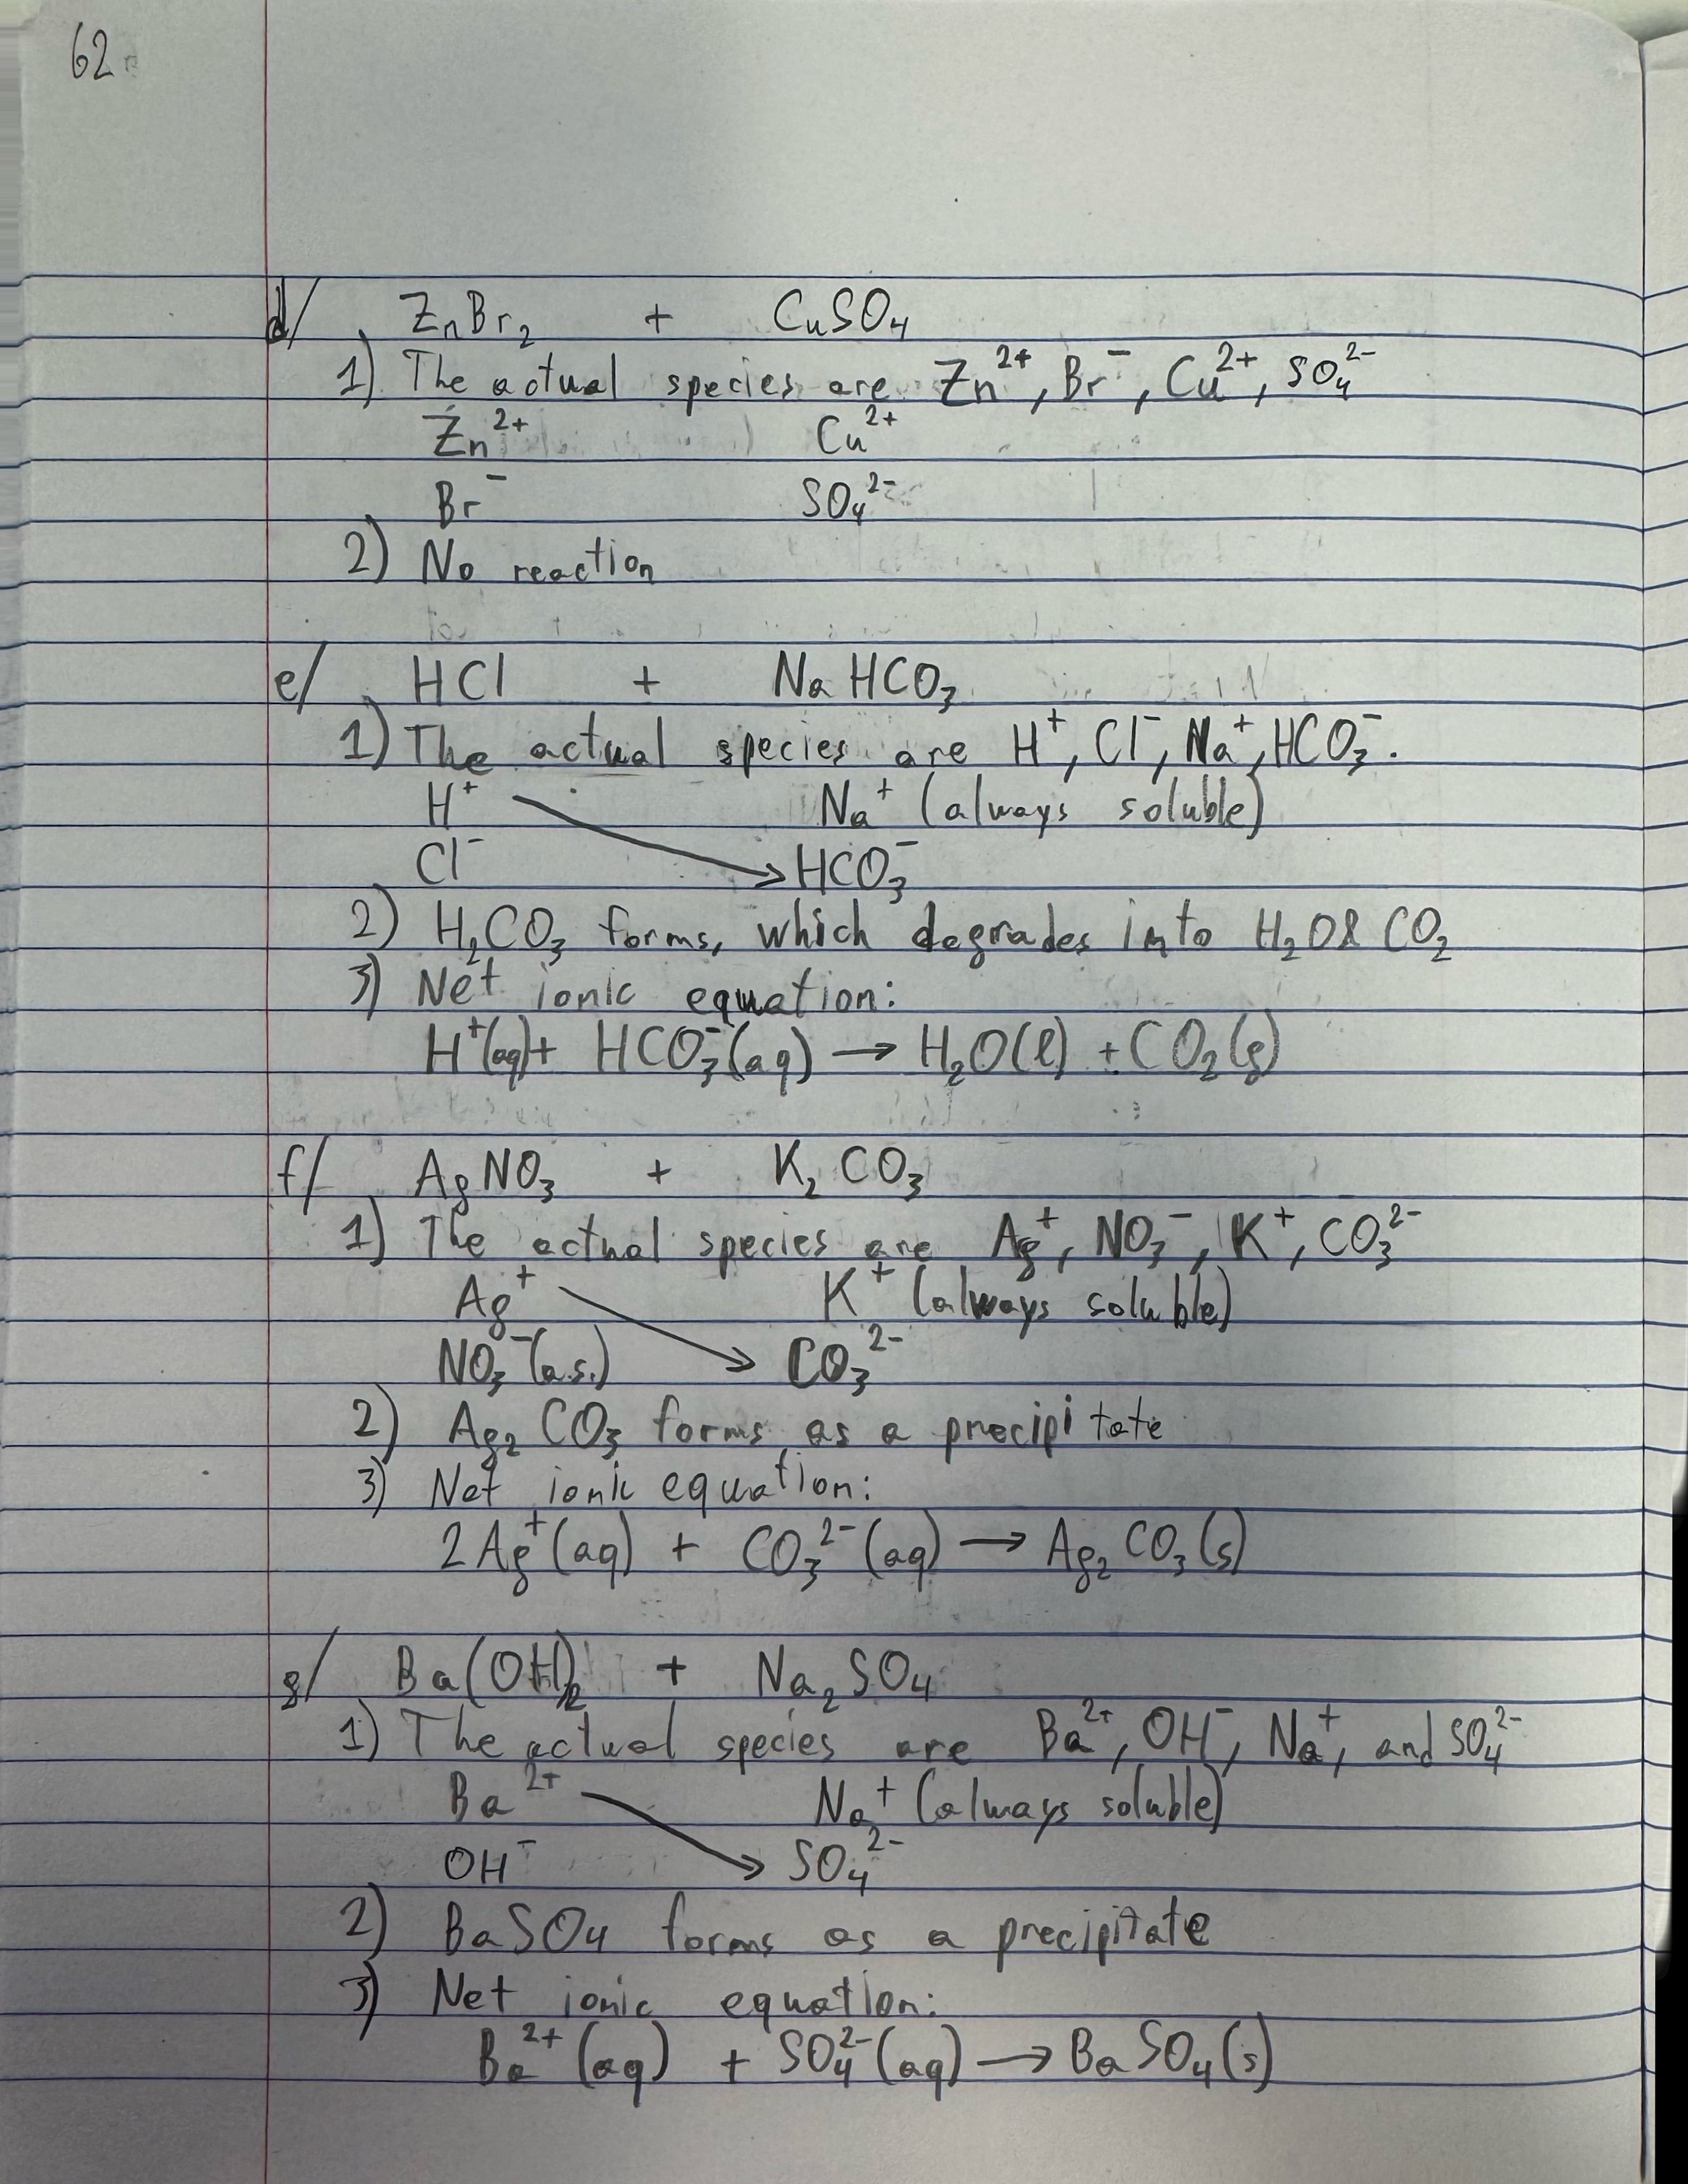
\includegraphics[width=\textwidth, trim={5in 2in 3in 39in},clip]{"Answers Images/IMG_6648.jpg"}

                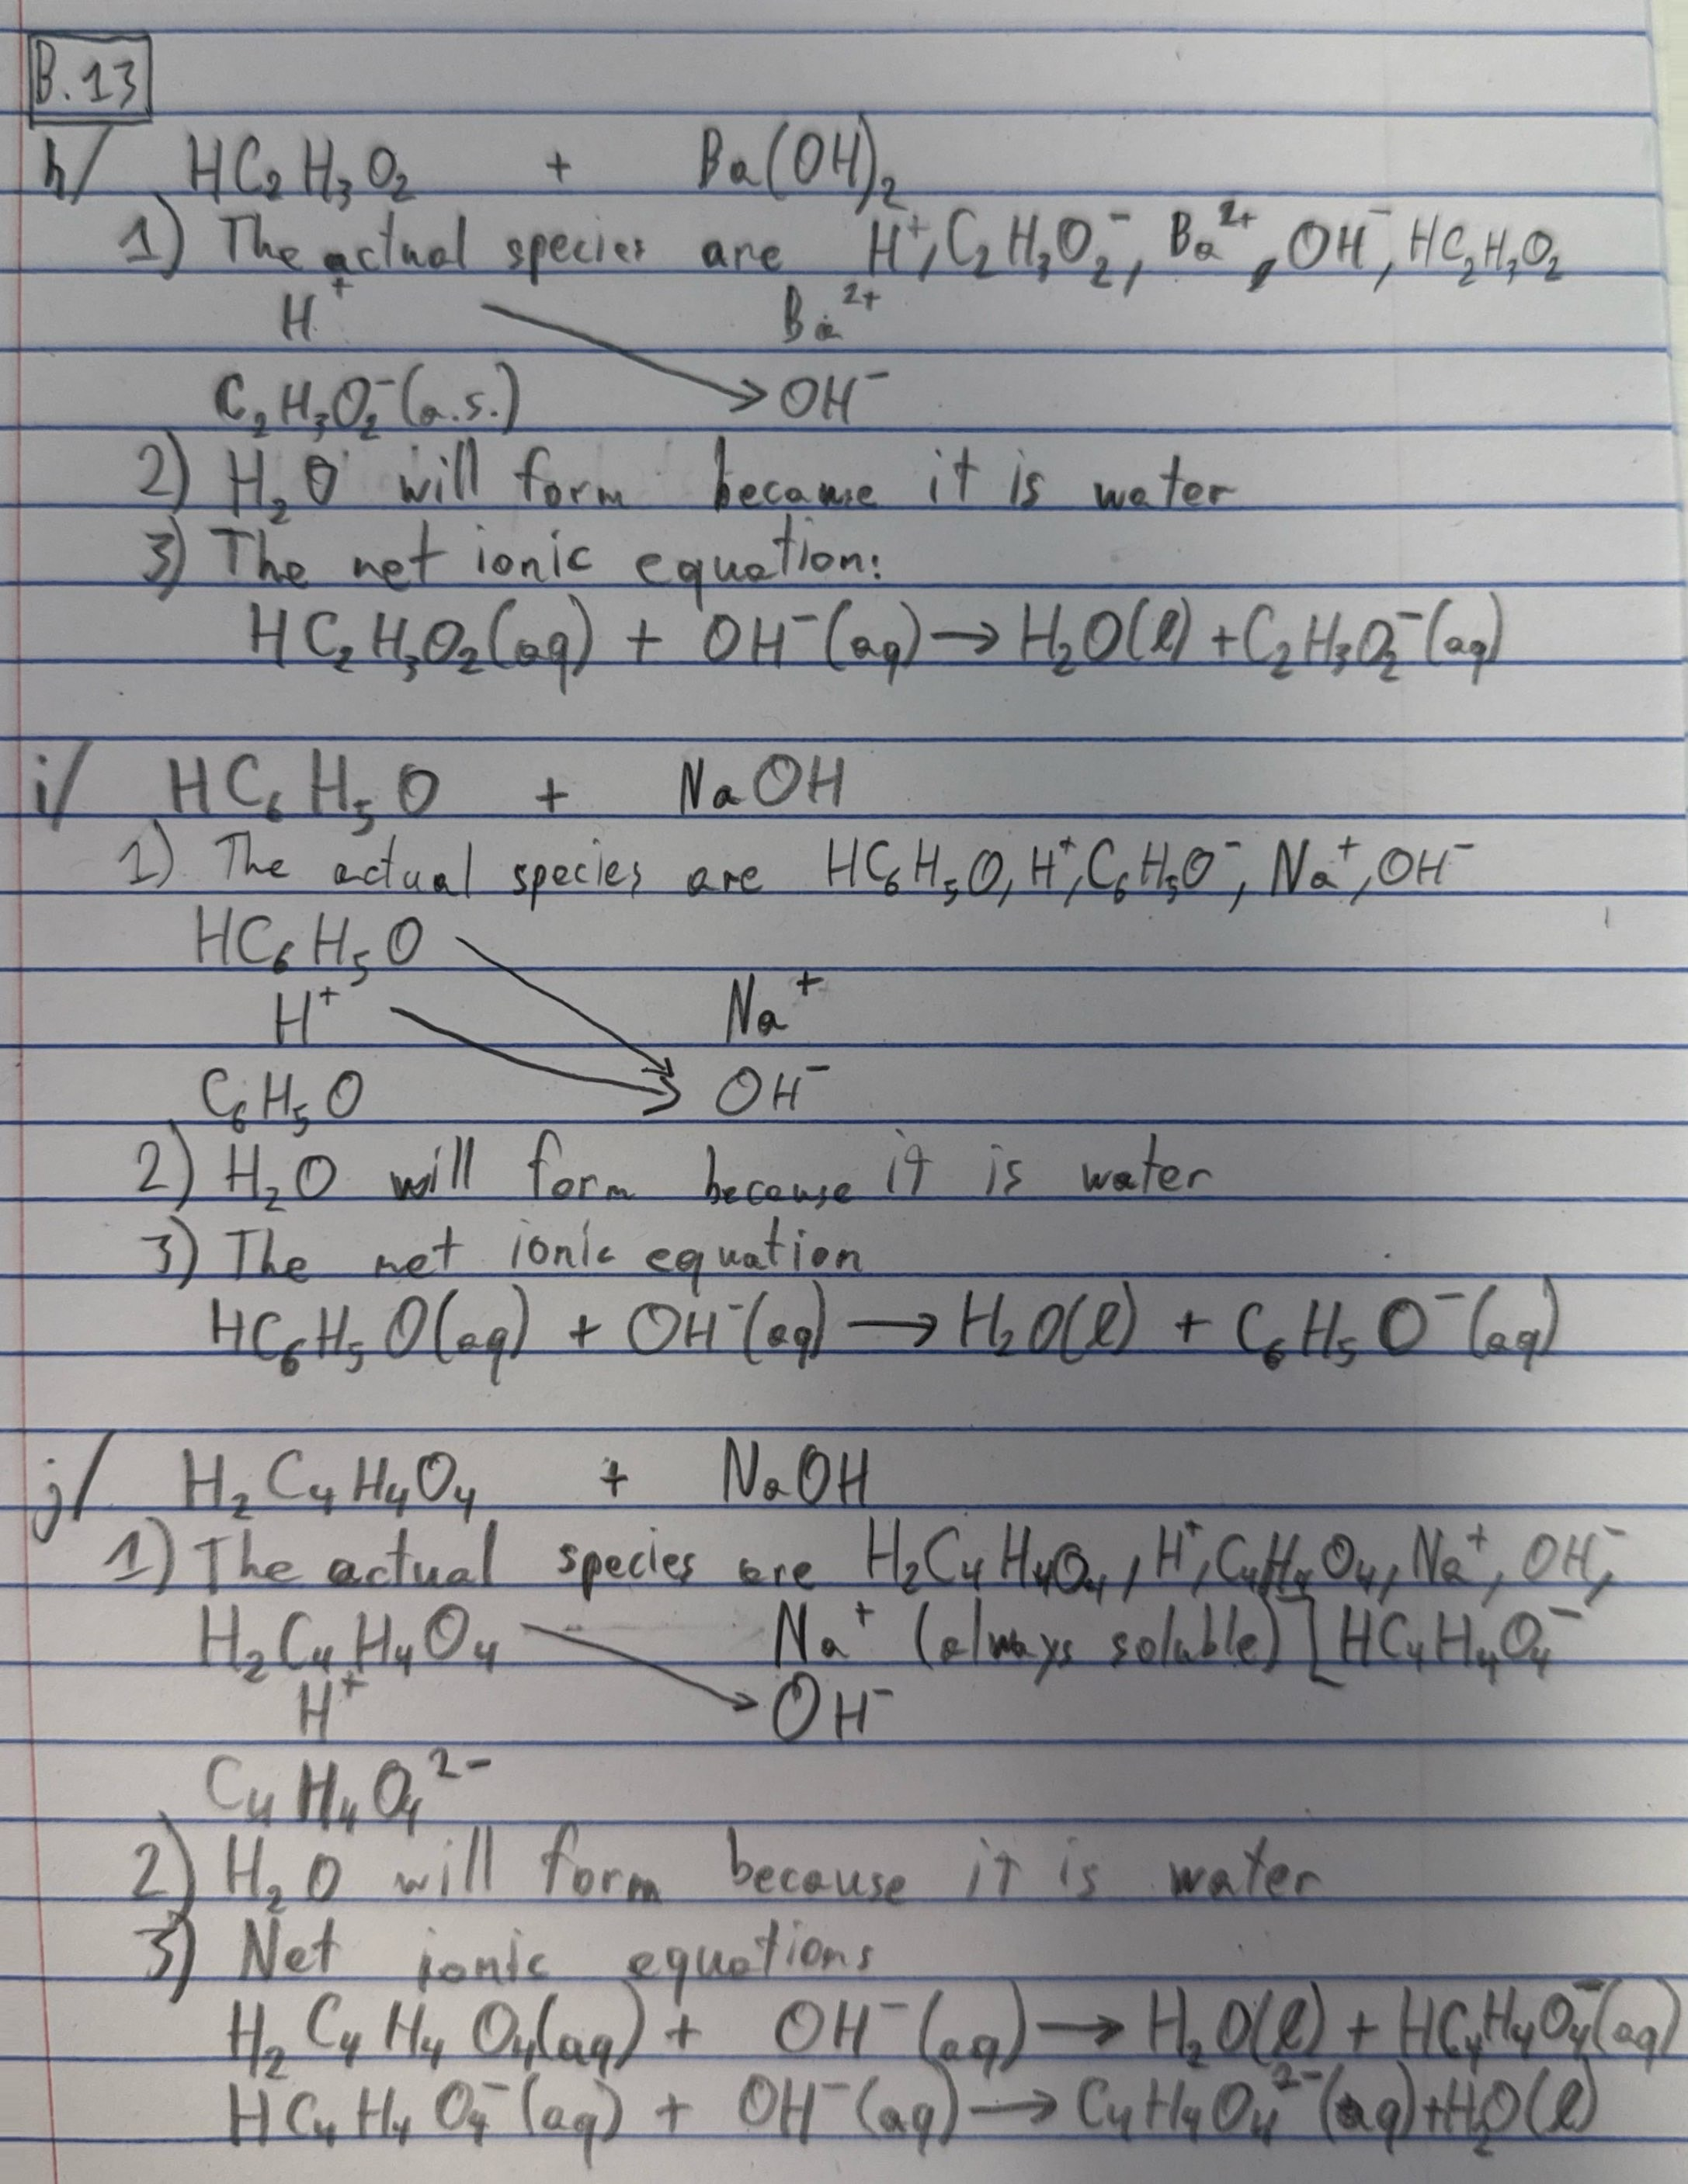
\includegraphics[width=\textwidth, trim={0in 0in 0in 2in},clip]{Answers Images/Scan Sep 1, 2025 at 18.06.jpg}
            \end{center}

    \pagebreak
    \section{Topic B Problem 14}
        Write balanced net ionic equations that explain the following observations.
        
        a) When solutions of \ce{BaCl2} and \ce{K2CrO4} are mixed, a bright yellow precipitate forms.
        
        b) When solutions of \ce{NaC12H22O2} and \ce{Ca(NO3)2} are mixed, a white precipitate forms.

        \subsection{Solution}
            \begin{center}
                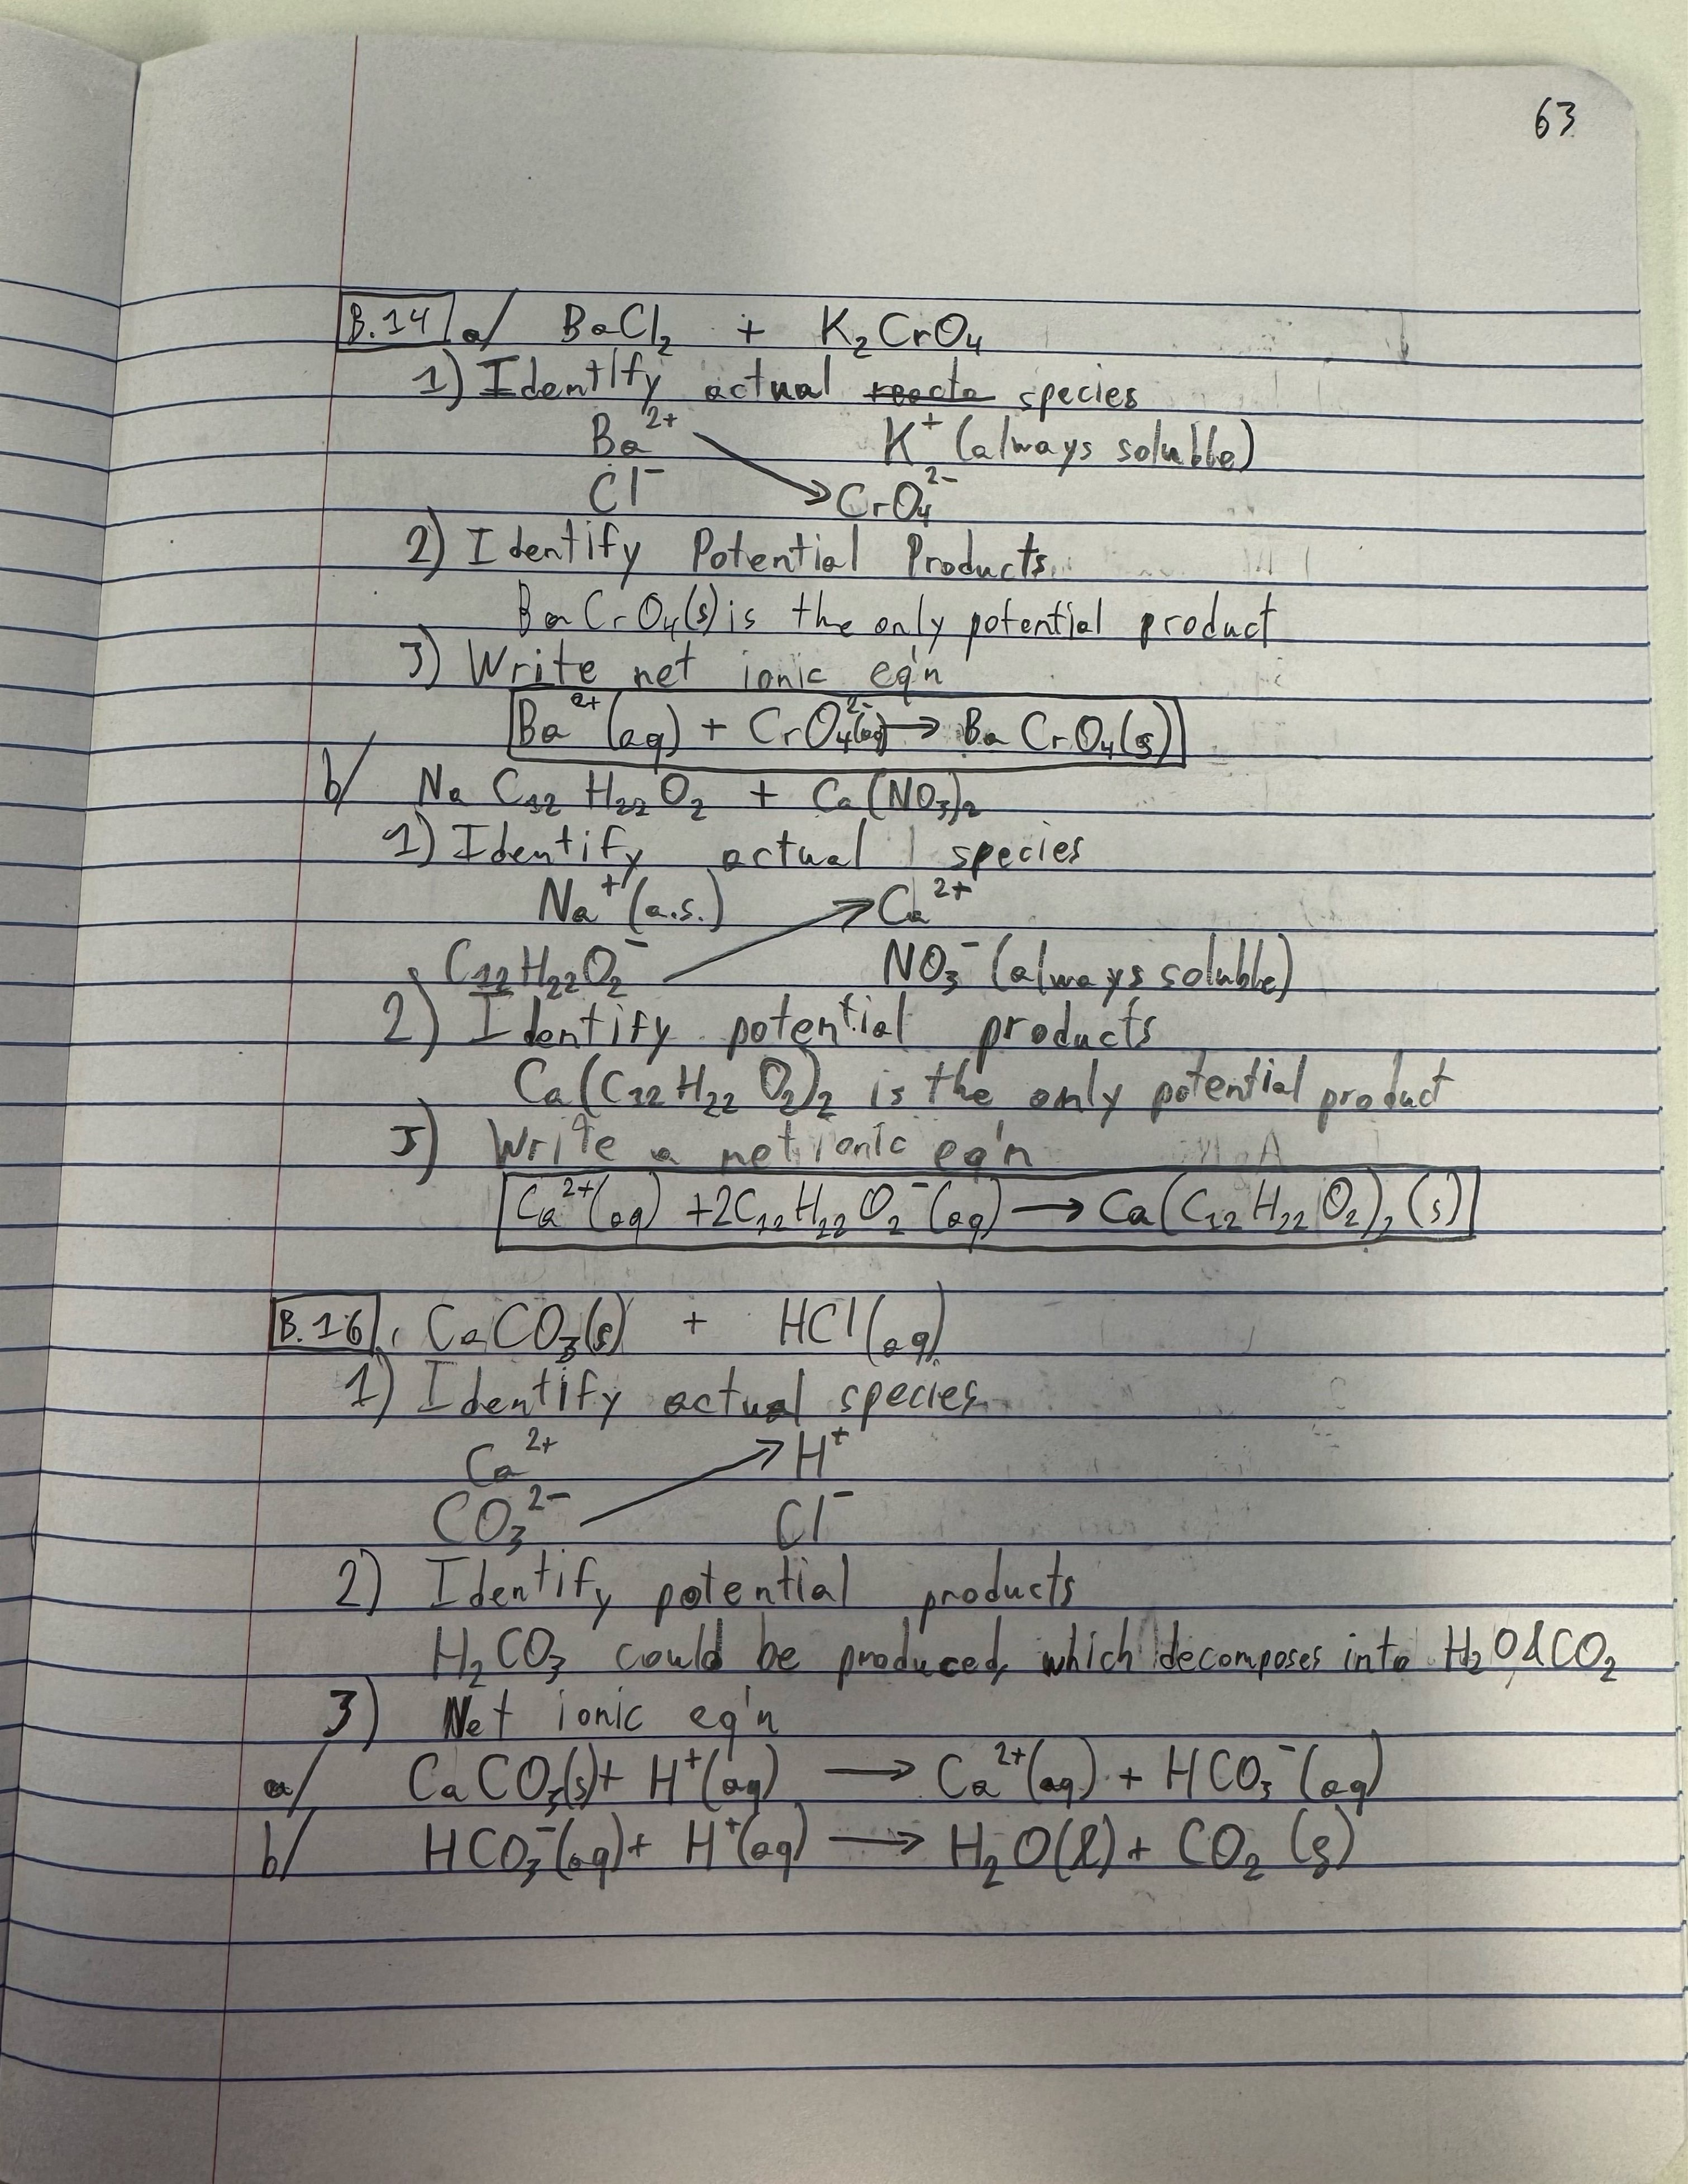
\includegraphics[width=\textwidth, trim={5in 23in 3in 7in},clip]{"Answers Images/IMG_6649.jpg"}
            \end{center}

    \pagebreak
    \section{Topic B Problem 15}
        Write the net ionic equation for the reaction that occurs when each of the following insoluble compounds is mixed with excess 6 M \ce{HCl}. 
        Be sure to include the state of each substance.
        \begin{multicols}{4}
            \begin{enumerate}[label=\alph*)]
                \item \ce{Mg(OH)2}
                \item \ce{CuO}
                \item \ce{Al(OH)3}
                \item \ce{Cr2O3}
            \end{enumerate}
        \end{multicols}

        \subsection{Solution (a)}
            \begin{center}
                \ce{Mg(OH)2 (aq) + 2H+ (aq) -> 2H2O(l) + Mg^2+ (aq)}
            \end{center}

        \subsection{Solution (b)}
            \begin{center}
                \ce{CuO (aq) + 2H+ (aq) -> H2O(l) + Cu+ (aq)}
            \end{center}

        \subsection{Solution (c)}
            \begin{center}
                \ce{Al(OH)3 (aq) + 3H+ (aq) -> 3H2O(l) + Mg^3+ (aq)}
            \end{center}

        \subsection{Solution (d)}
            \begin{center}
                \ce{Cr2O3 (aq) + 6H+ (aq) -> 3H2O(l) + 2Cr^3+ (aq)}
            \end{center}

    \pagebreak
    \section{Topic B Problem 16}
        If you put some solid \ce{CaCO3} into a beaker of water and slowly add \ce{HCl} solution, stirring vigorously the whole time, the \ce{CaCO3} gradually dissolves. 
        As the last of the \ce{CaCO3} dissolves, bubbles begin to form, and if you continue to add \ce{HCl}, you observe steady bubble formation.
        
        a) Write a net ionic equation that shows why the \ce{CaCO3} dissolves.
        
        b) Write a net ionic equation that shows why the mixture bubbles.

        \subsection{Solution}
            \begin{center}
                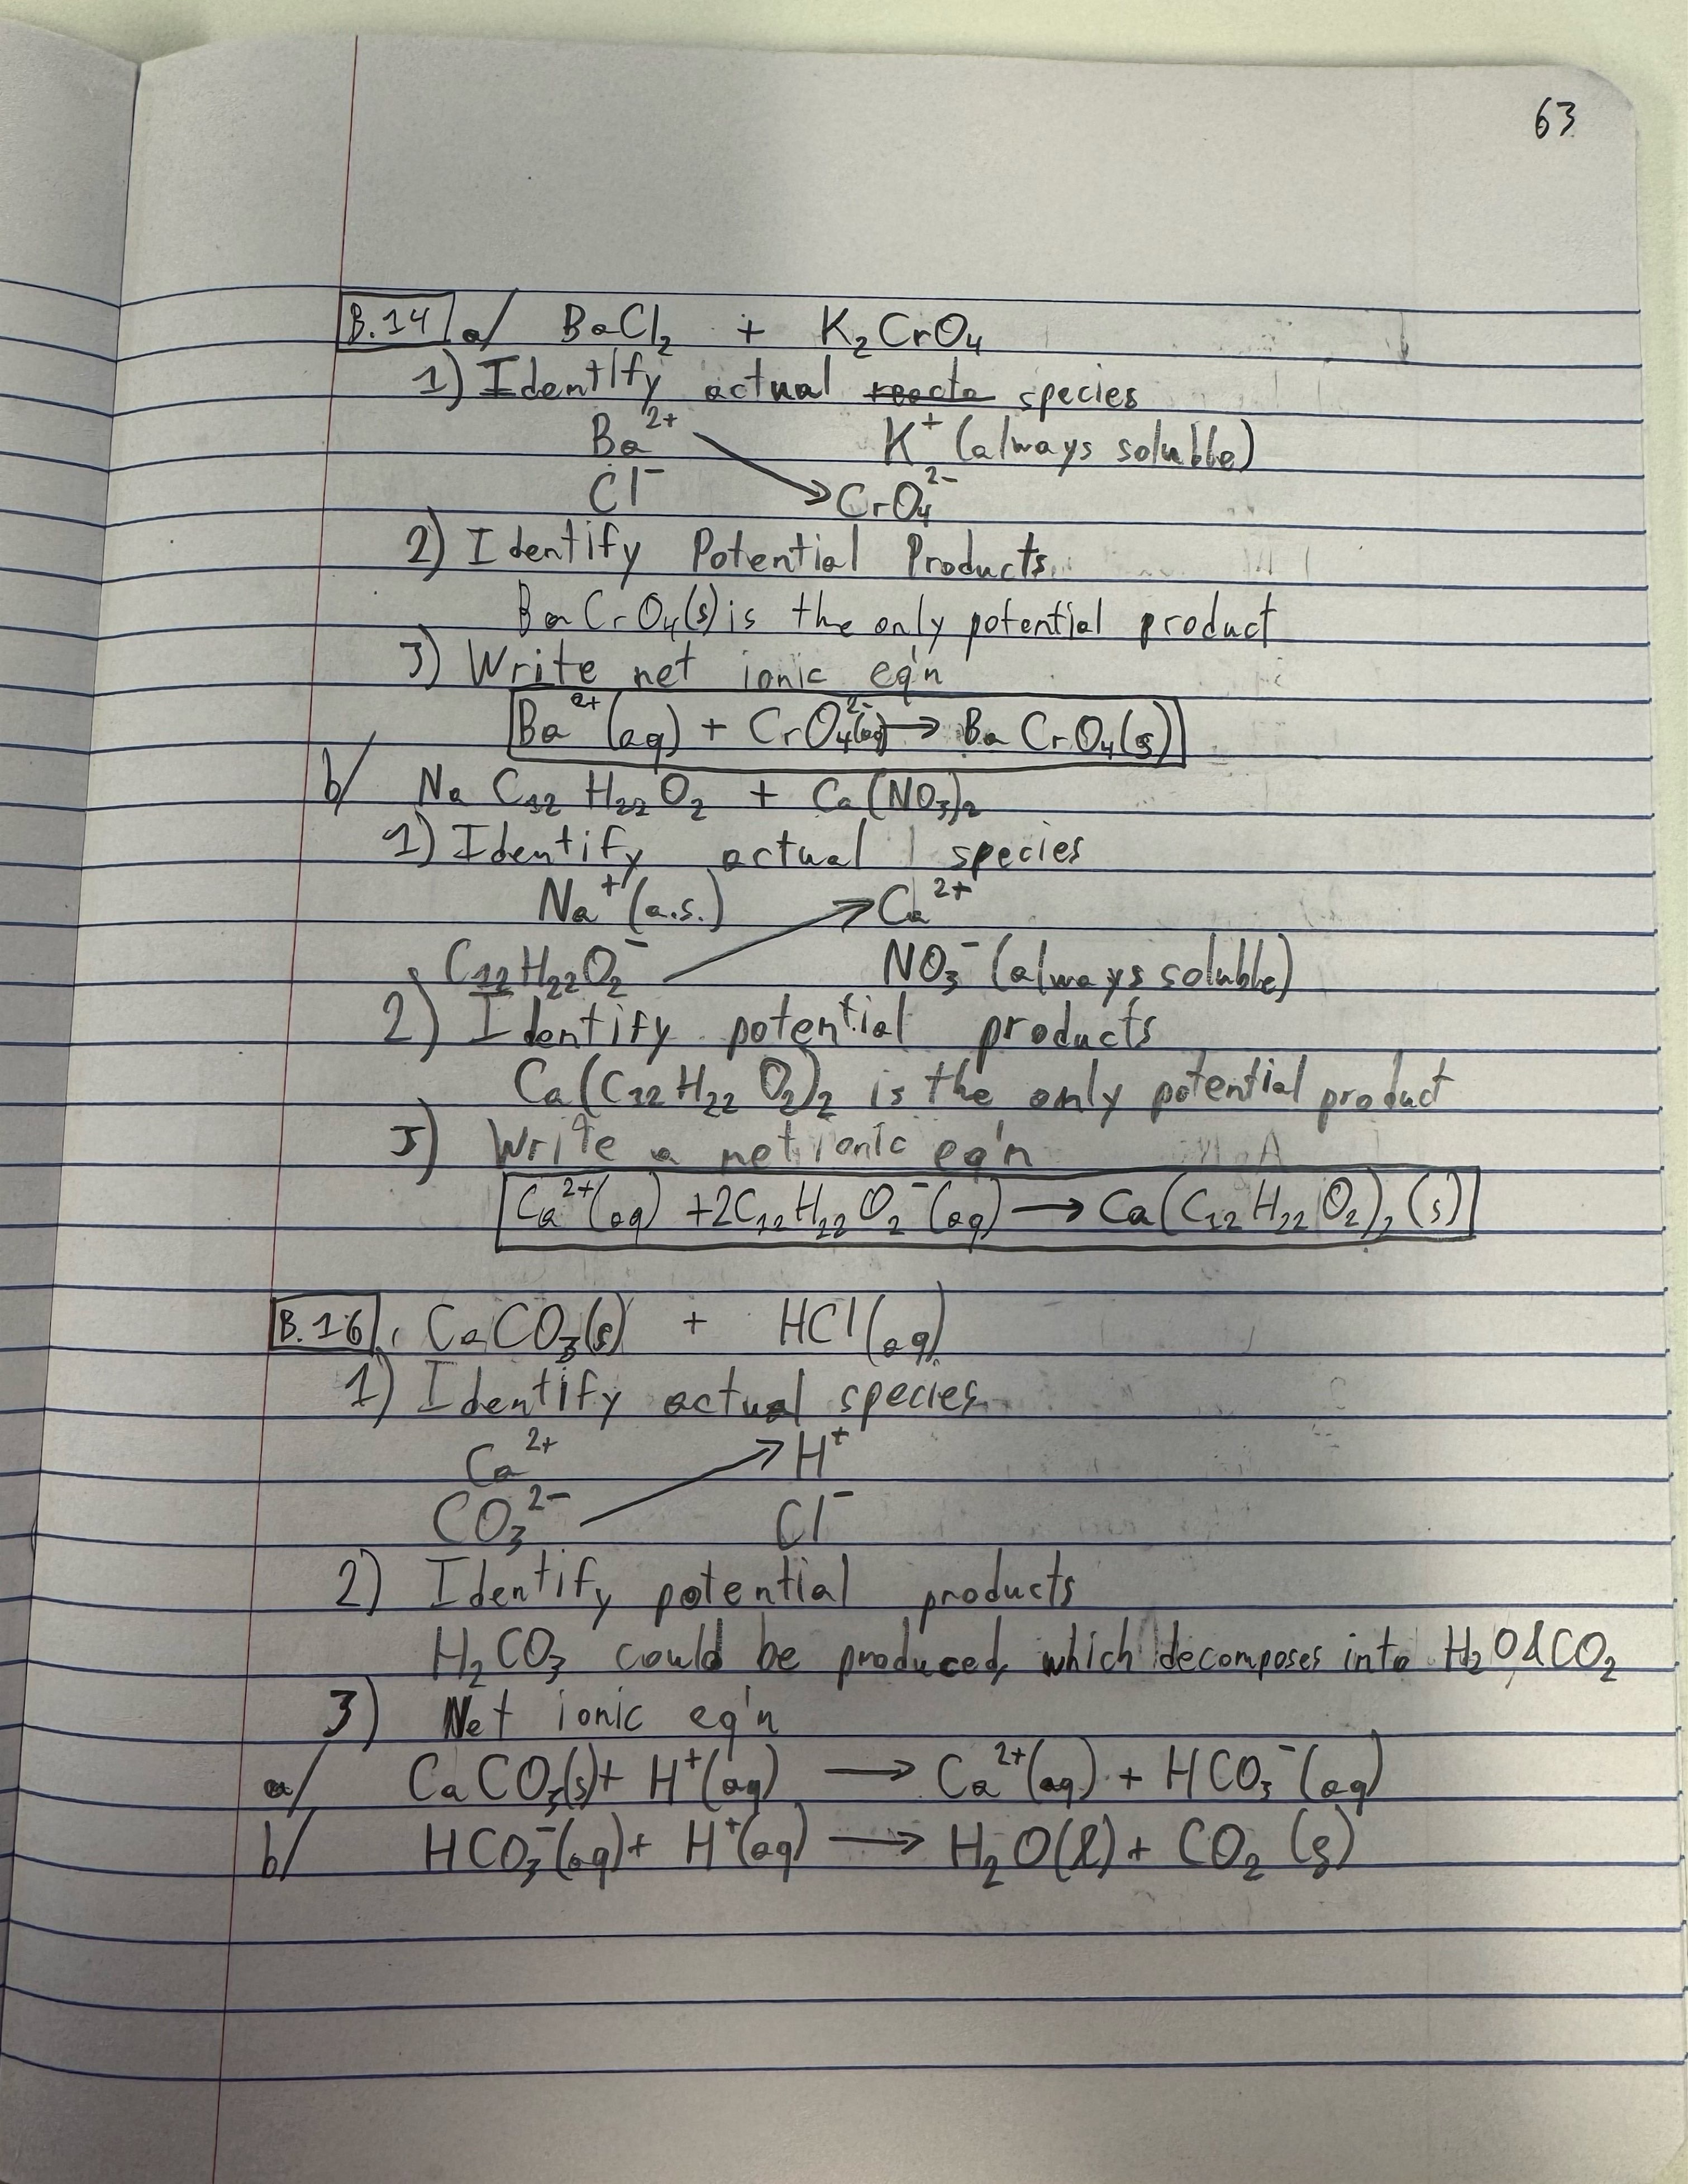
\includegraphics[width=\textwidth, trim={5in 7in 1in 32in},clip]{"Answers Images/IMG_6649.jpg"}
            \end{center}

            Note (a): The reason that the above equation shows that \ce{CaCO3} dissolves is because the two results are both aqeous.

            Note (b): The reason that the above equation shows why it produces bubbles is because it contains \ce{CO2}, which which is a gas that would create bubbles.

    \pagebreak
    \section{Topic B Problem 17}
        Both \ce{MgO} and \ce{PbO} are insoluble in water. When solid \ce{MgO} is added to 3 M \ce{H2SO4}, the solid dissolves completely. 
        When solid PbO is added to 3 M \ce{H2SO4}, the solid changes color slightly, but does not dissolve. 
        Explain this difference.

        \subsection{Solution}
            The \ce{MgO} and the \ce{PbO} would react with the \ce{SO4^2-}.
            The \ce{O} would in both cases react to form \ce{H2O}, while the other cations would be attracted to the \ce{SO4^2-}.
            \ce{SO4^2-} is solube with \ce{Mg^2+}, while it would be insoluble with \ce{Pb^2+}. 
            This is what causes the solid of \ce{PbO} to change color: it is turning into \ce{PbSO4}. 
            Meanwhile, the \ce{MgO} would be turning into fully soluble \ce{MgSO4}.

    \pagebreak
    \section{Topic B Problem 18}
        A solution contains one or more of the following anions: \ce{I-}, \ce{PO4^3-}, and \ce{NO3-}. 
        A chemist carries out the following experiments on this solution:
        \begin{itemize}
            \item Experiment 1: The chemist adds 0.1 M \ce{Ba(NO3)2} to a small portion of this solution, and no precipitate forms.
            \item Experiment 2: The chemist adds 0.1 M \ce{AgNO3} to the solution from Experiment 1, and a precipitate forms.
        \end{itemize}
        Based on these results, tell which anions are definitely present in the original solution, which anions are definitely absent from the original solution, and which anions cannot be determined from the information given here. 
        Explain your answer.

        \subsection{Solution}
            \begin{center}
                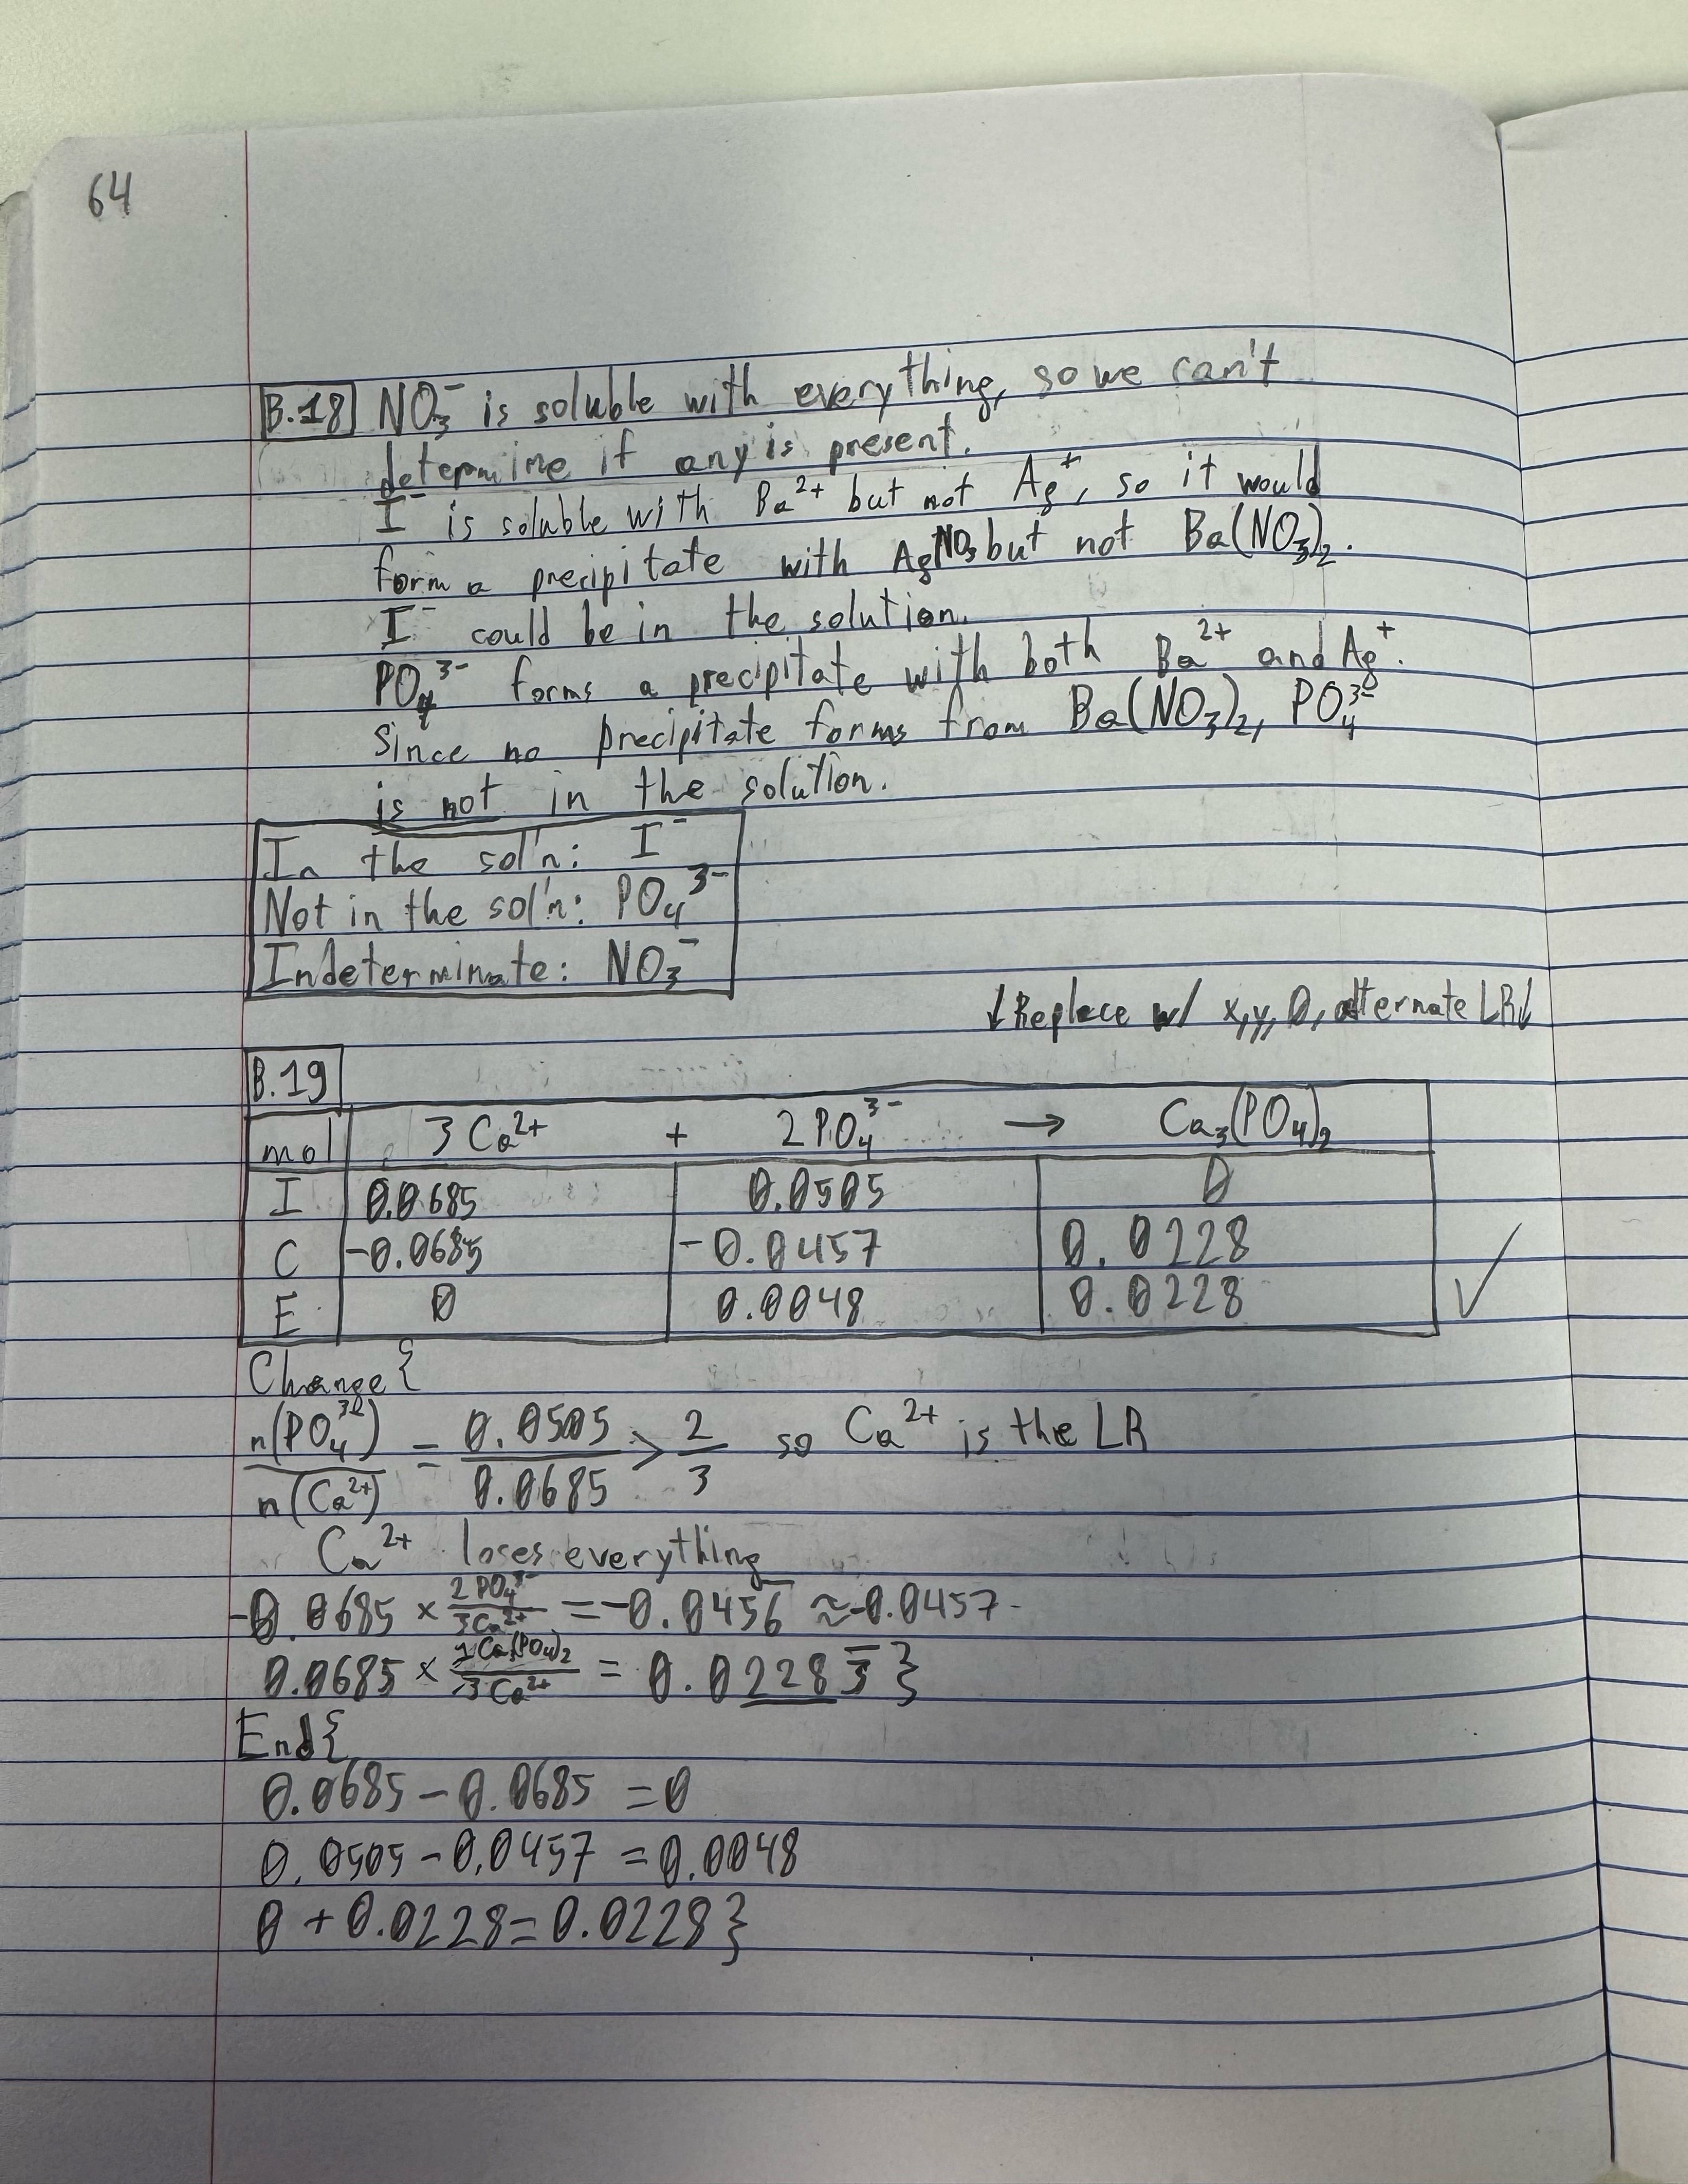
\includegraphics[width=\textwidth, trim={5in 30in 3in 7in},clip]{"Answers Images/IMG_6650.jpg"}
            \end{center}

    \pagebreak
    \section{Topic B Problem 19}
        Complete the following ICE table:

        \begin{center}
            \begin{tabular}{|c|c@{}c@{}c@{}c@{}c|}
                \hline
                mol &   \ce{3 Ca^2+} & ${}+{}$ & \ce{3 PO4^3-} & ${}\rightarrow{}$ & \ce{Ca3(PO4)2} \\
                \hline
                I   &   0.0685      &&              0.0505                          &&  0           \\
                C   &               &&                                              &&              \\
                E   &               &&                                              &&              \\
                \hline
            \end{tabular}
        \end{center}

        \subsection{Solution}
            \begin{center}
                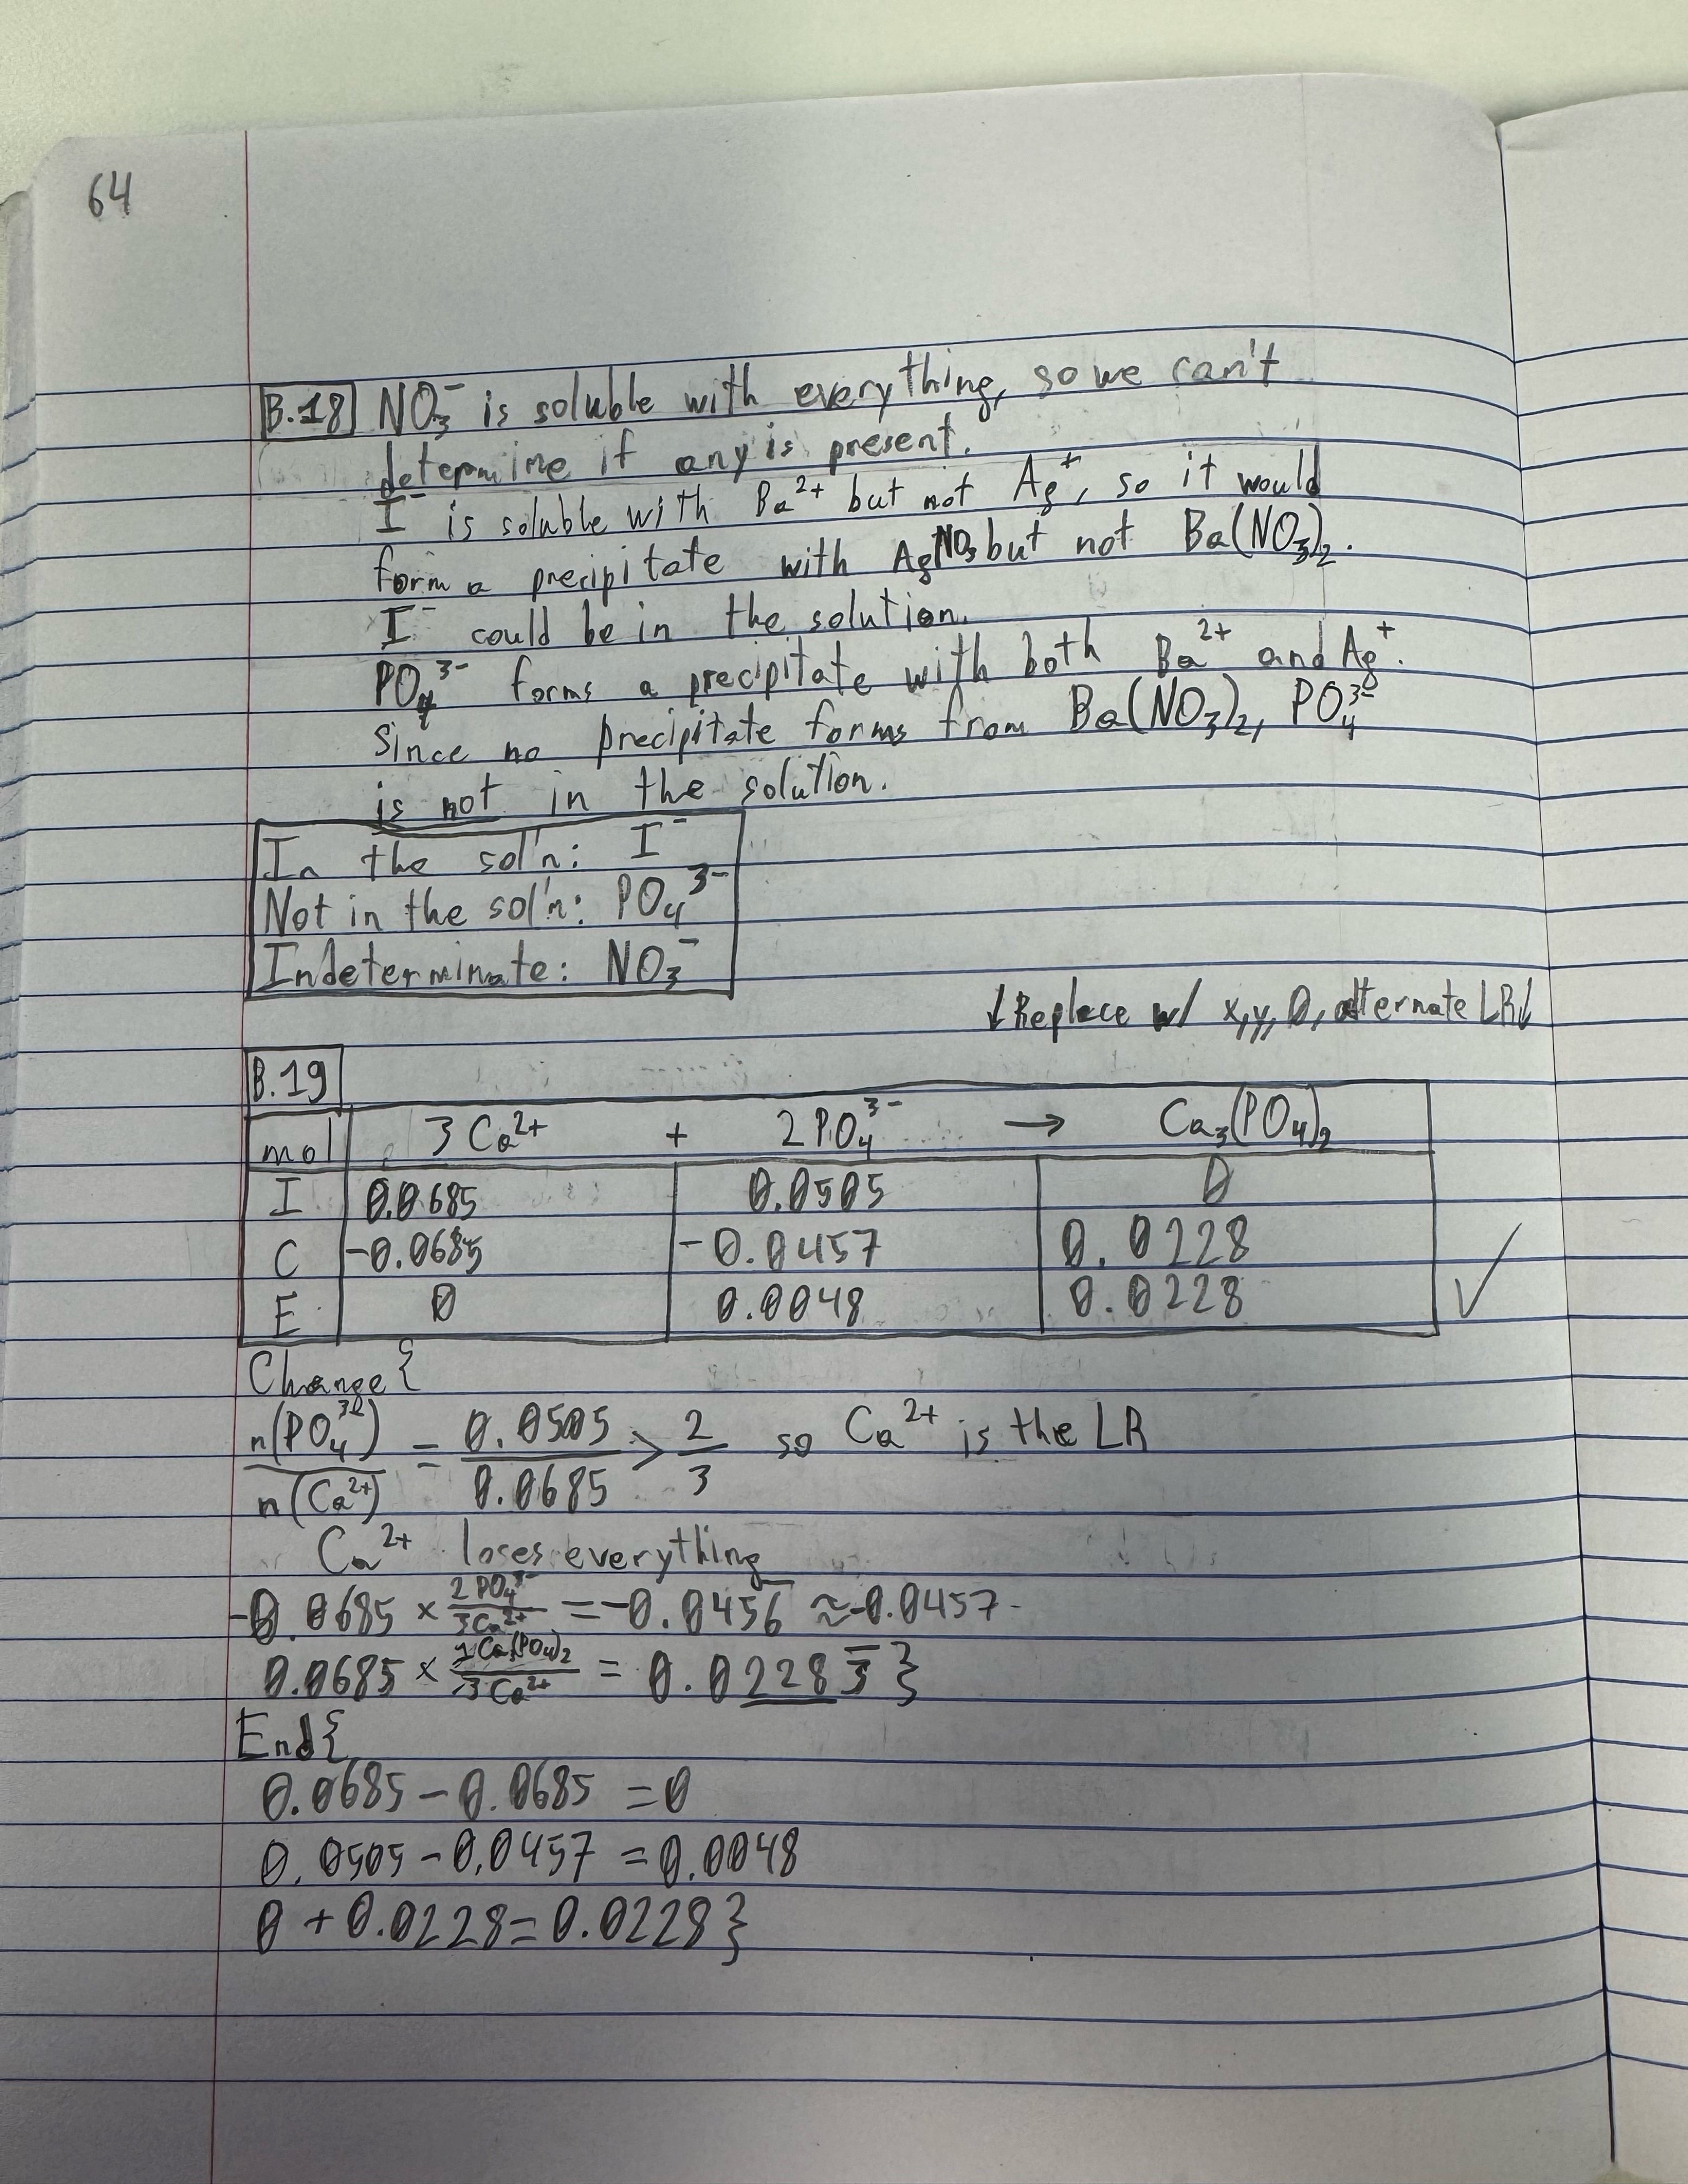
\includegraphics[width=\textwidth, trim={5in 5in 3in 27in},clip]{"Answers Images/IMG_6650.jpg"}
            \end{center}

    \pagebreak
    \section{Topic B Problem 20}
        Complete the following ICE table, assuming \ce{Ca^2+} is the limiting reactant:

        \begin{center}
            \begin{tabular}{|c|c@{}c@{}c@{}c@{}c|}
                \hline
                mol &   \ce{3 Ca^2+} & ${}+{}$ & \ce{3 PO4^3-} & ${}\rightarrow{}$ & \ce{Ca3(PO4)2} \\
                \hline
                I   &   \textbf{x}  &&              \textbf{y}                      &&  0           \\
                C   &               &&                                              &&              \\
                E   &               &&                                              &&              \\
                \hline
            \end{tabular}
        \end{center}

        \subsection{Solution}
            \begin{center}
                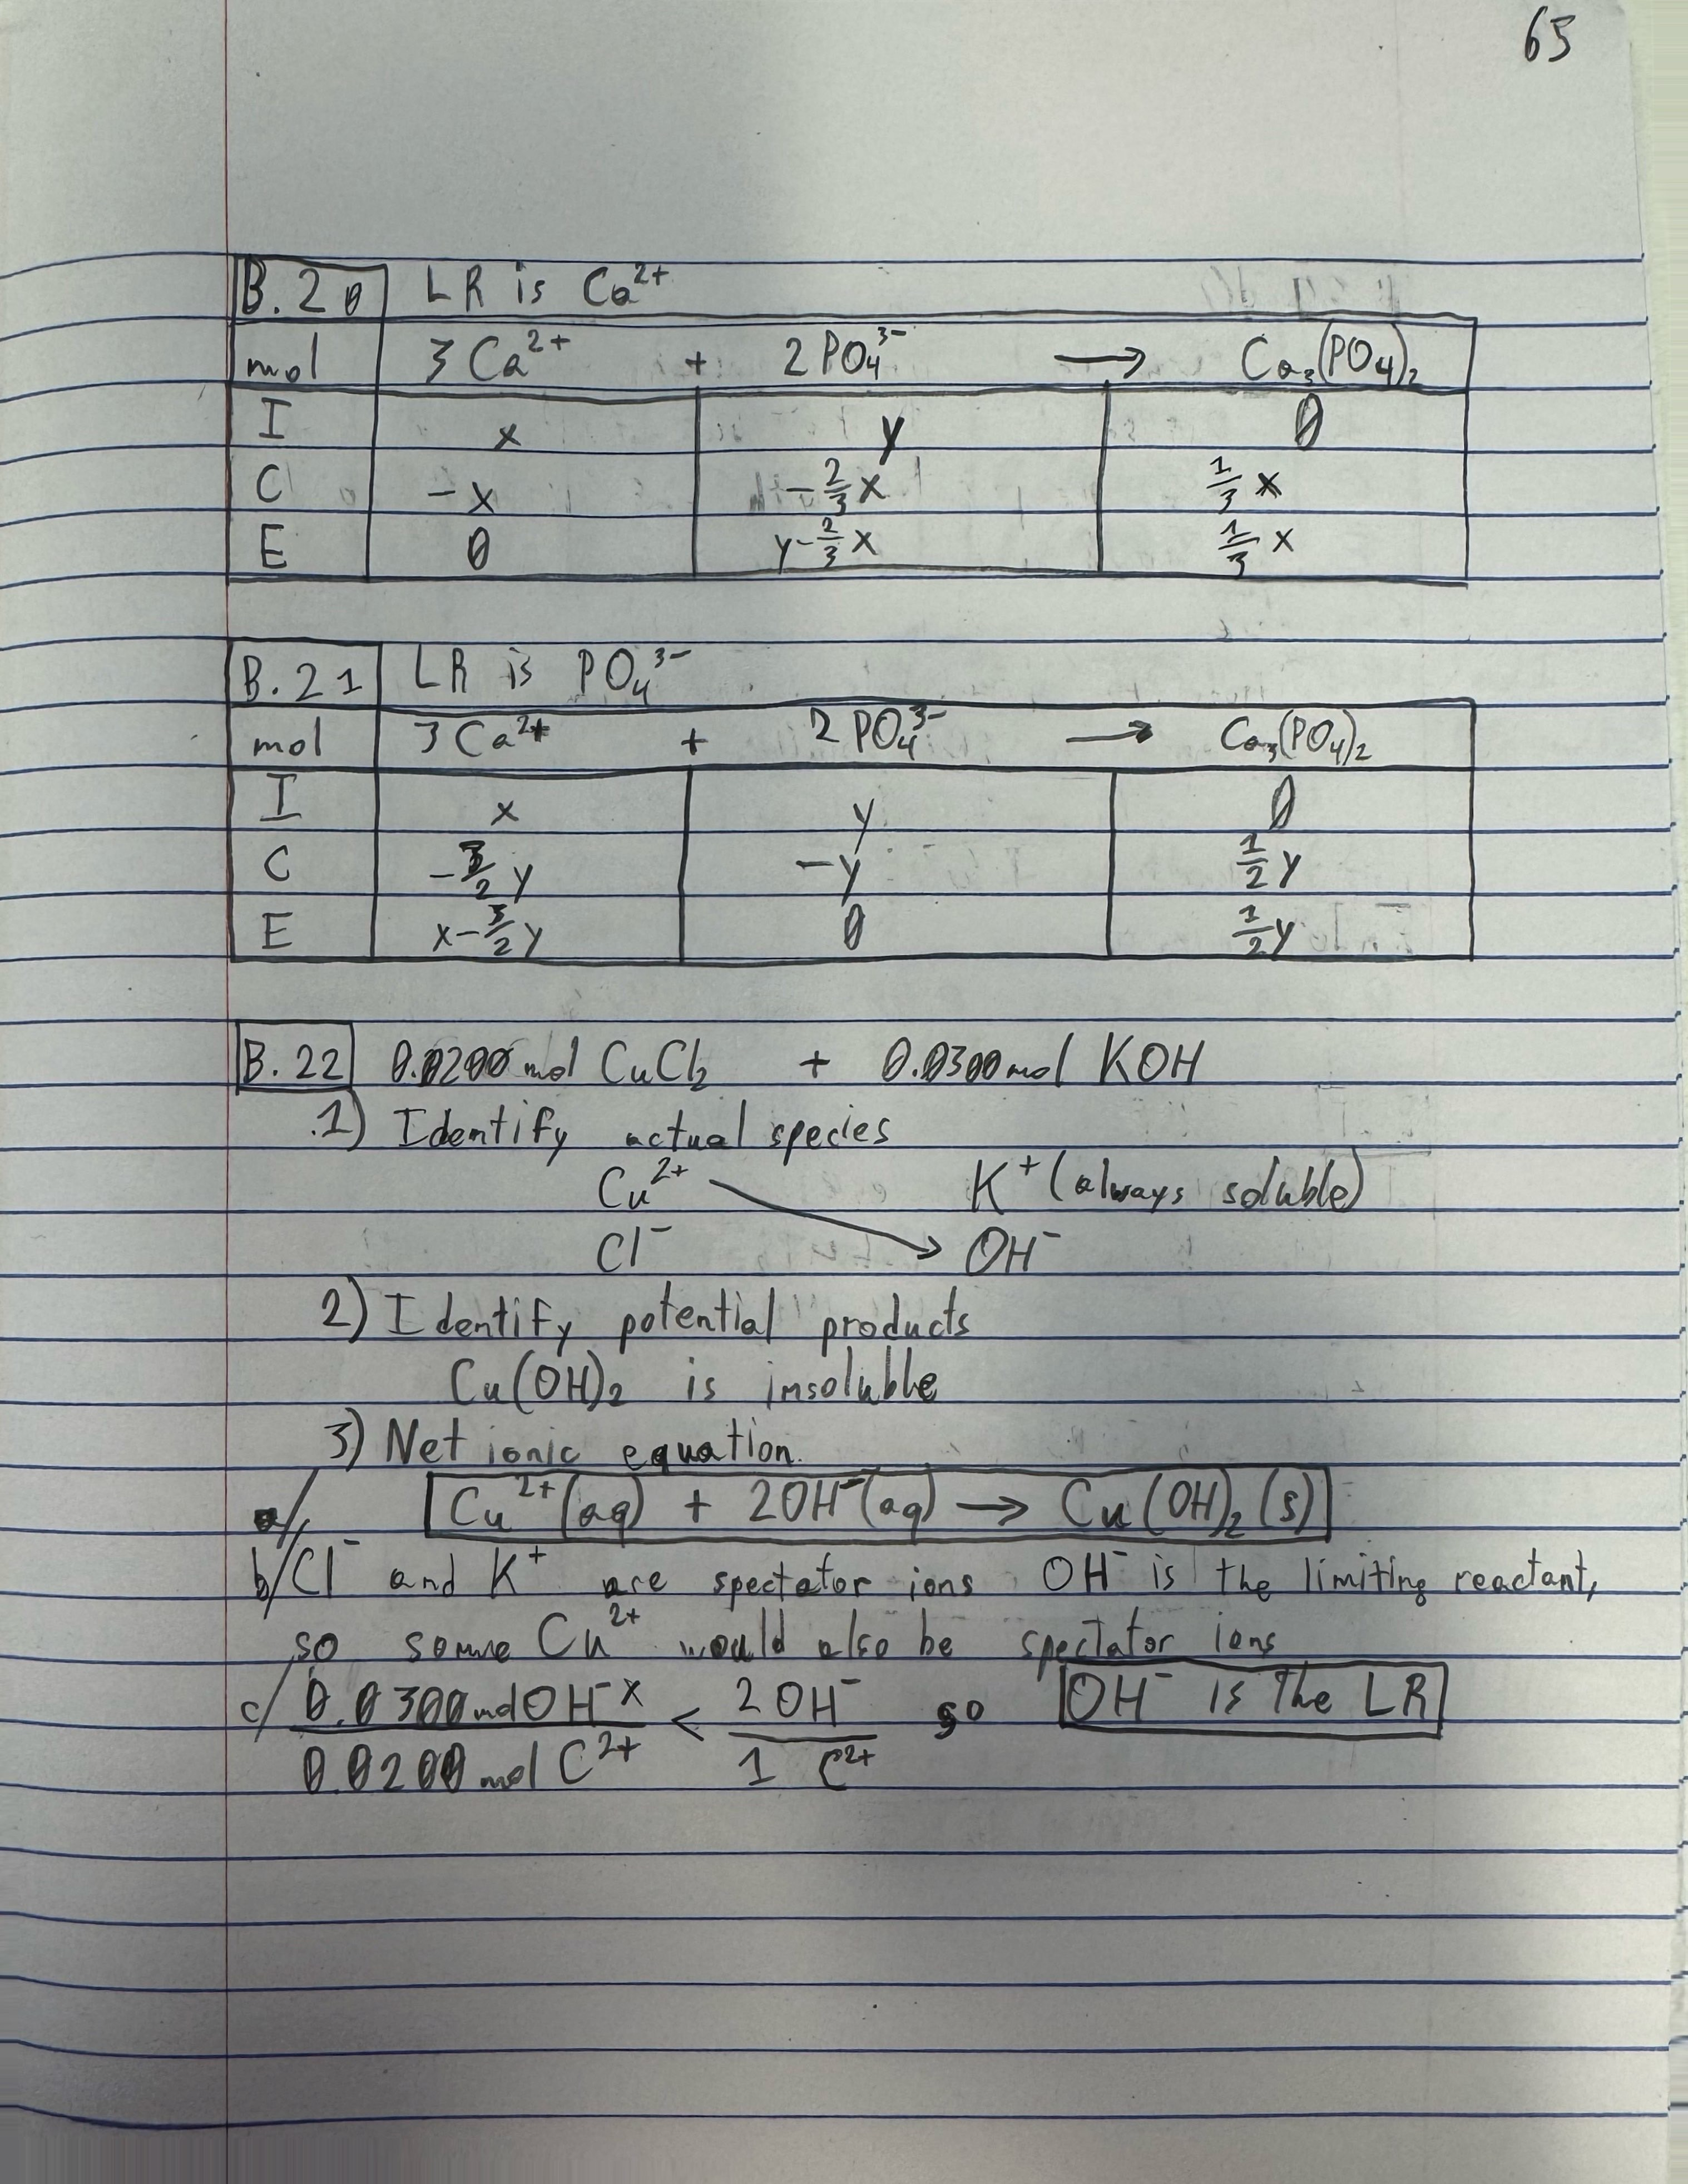
\includegraphics[width=\textwidth, trim={5in 40in 3in 5in},clip]{"Answers Images/IMG_6651.jpg"}
            \end{center}

    \pagebreak
    \section{Topic B Problem 21}
        Repeat Problem 20, but now assume that \ce{PO4^3-} is the limiting reactant.

        \subsection{Solution}
            \begin{center}
                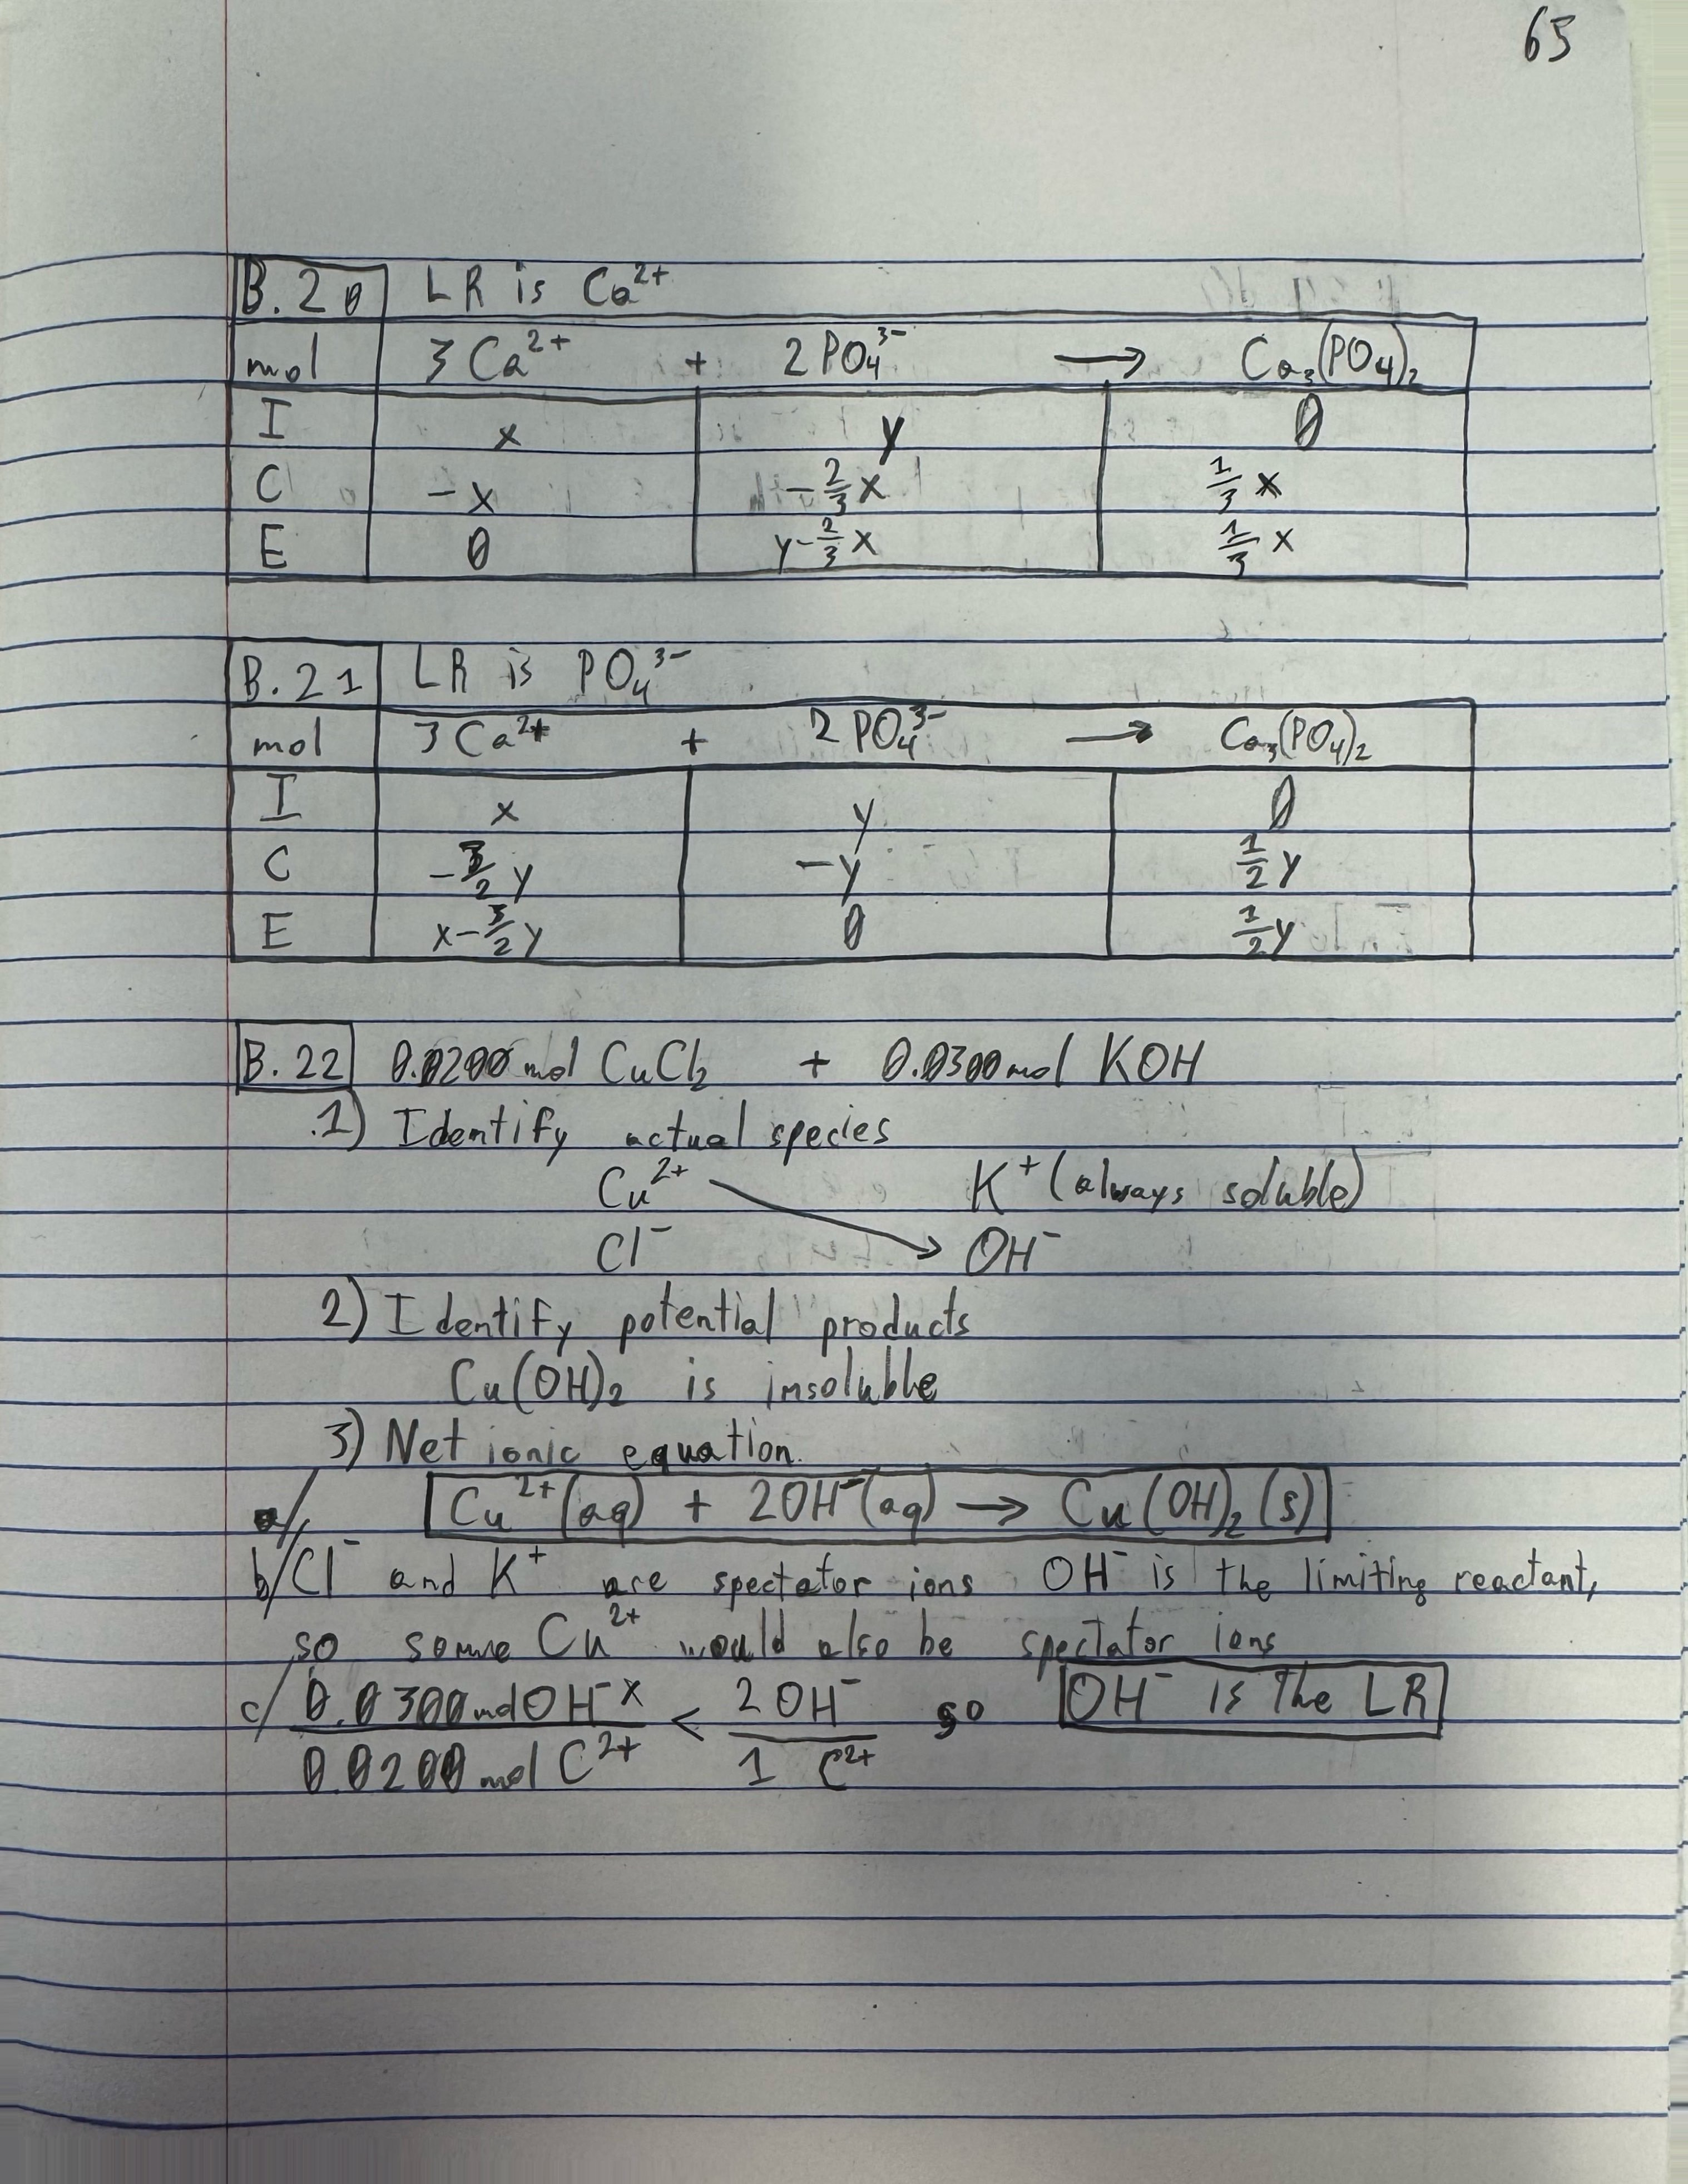
\includegraphics[width=\textwidth, trim={5in 30in 3in 15in},clip]{"Answers Images/IMG_6651.jpg"}
            \end{center}

    \pagebreak
    \section{Topic B Problem 22}
        A chemist prepares a mixture that contains 0.0200 mol of \ce{CuCl2} and 0.0300 mol of \ce{KOH} dissolved in water.
        
        a) Write the balanced net ionic equation for the reaction that occurs.
        
        b) What are the spectator ions in this reaction?
        
        c) What is the limiting reactant in this reaction? (Hint: it's an ion.)
        
        d) Construct an ICE table for this reaction, using the net ionic equation.

        \subsection{Solution}
            \begin{center}
                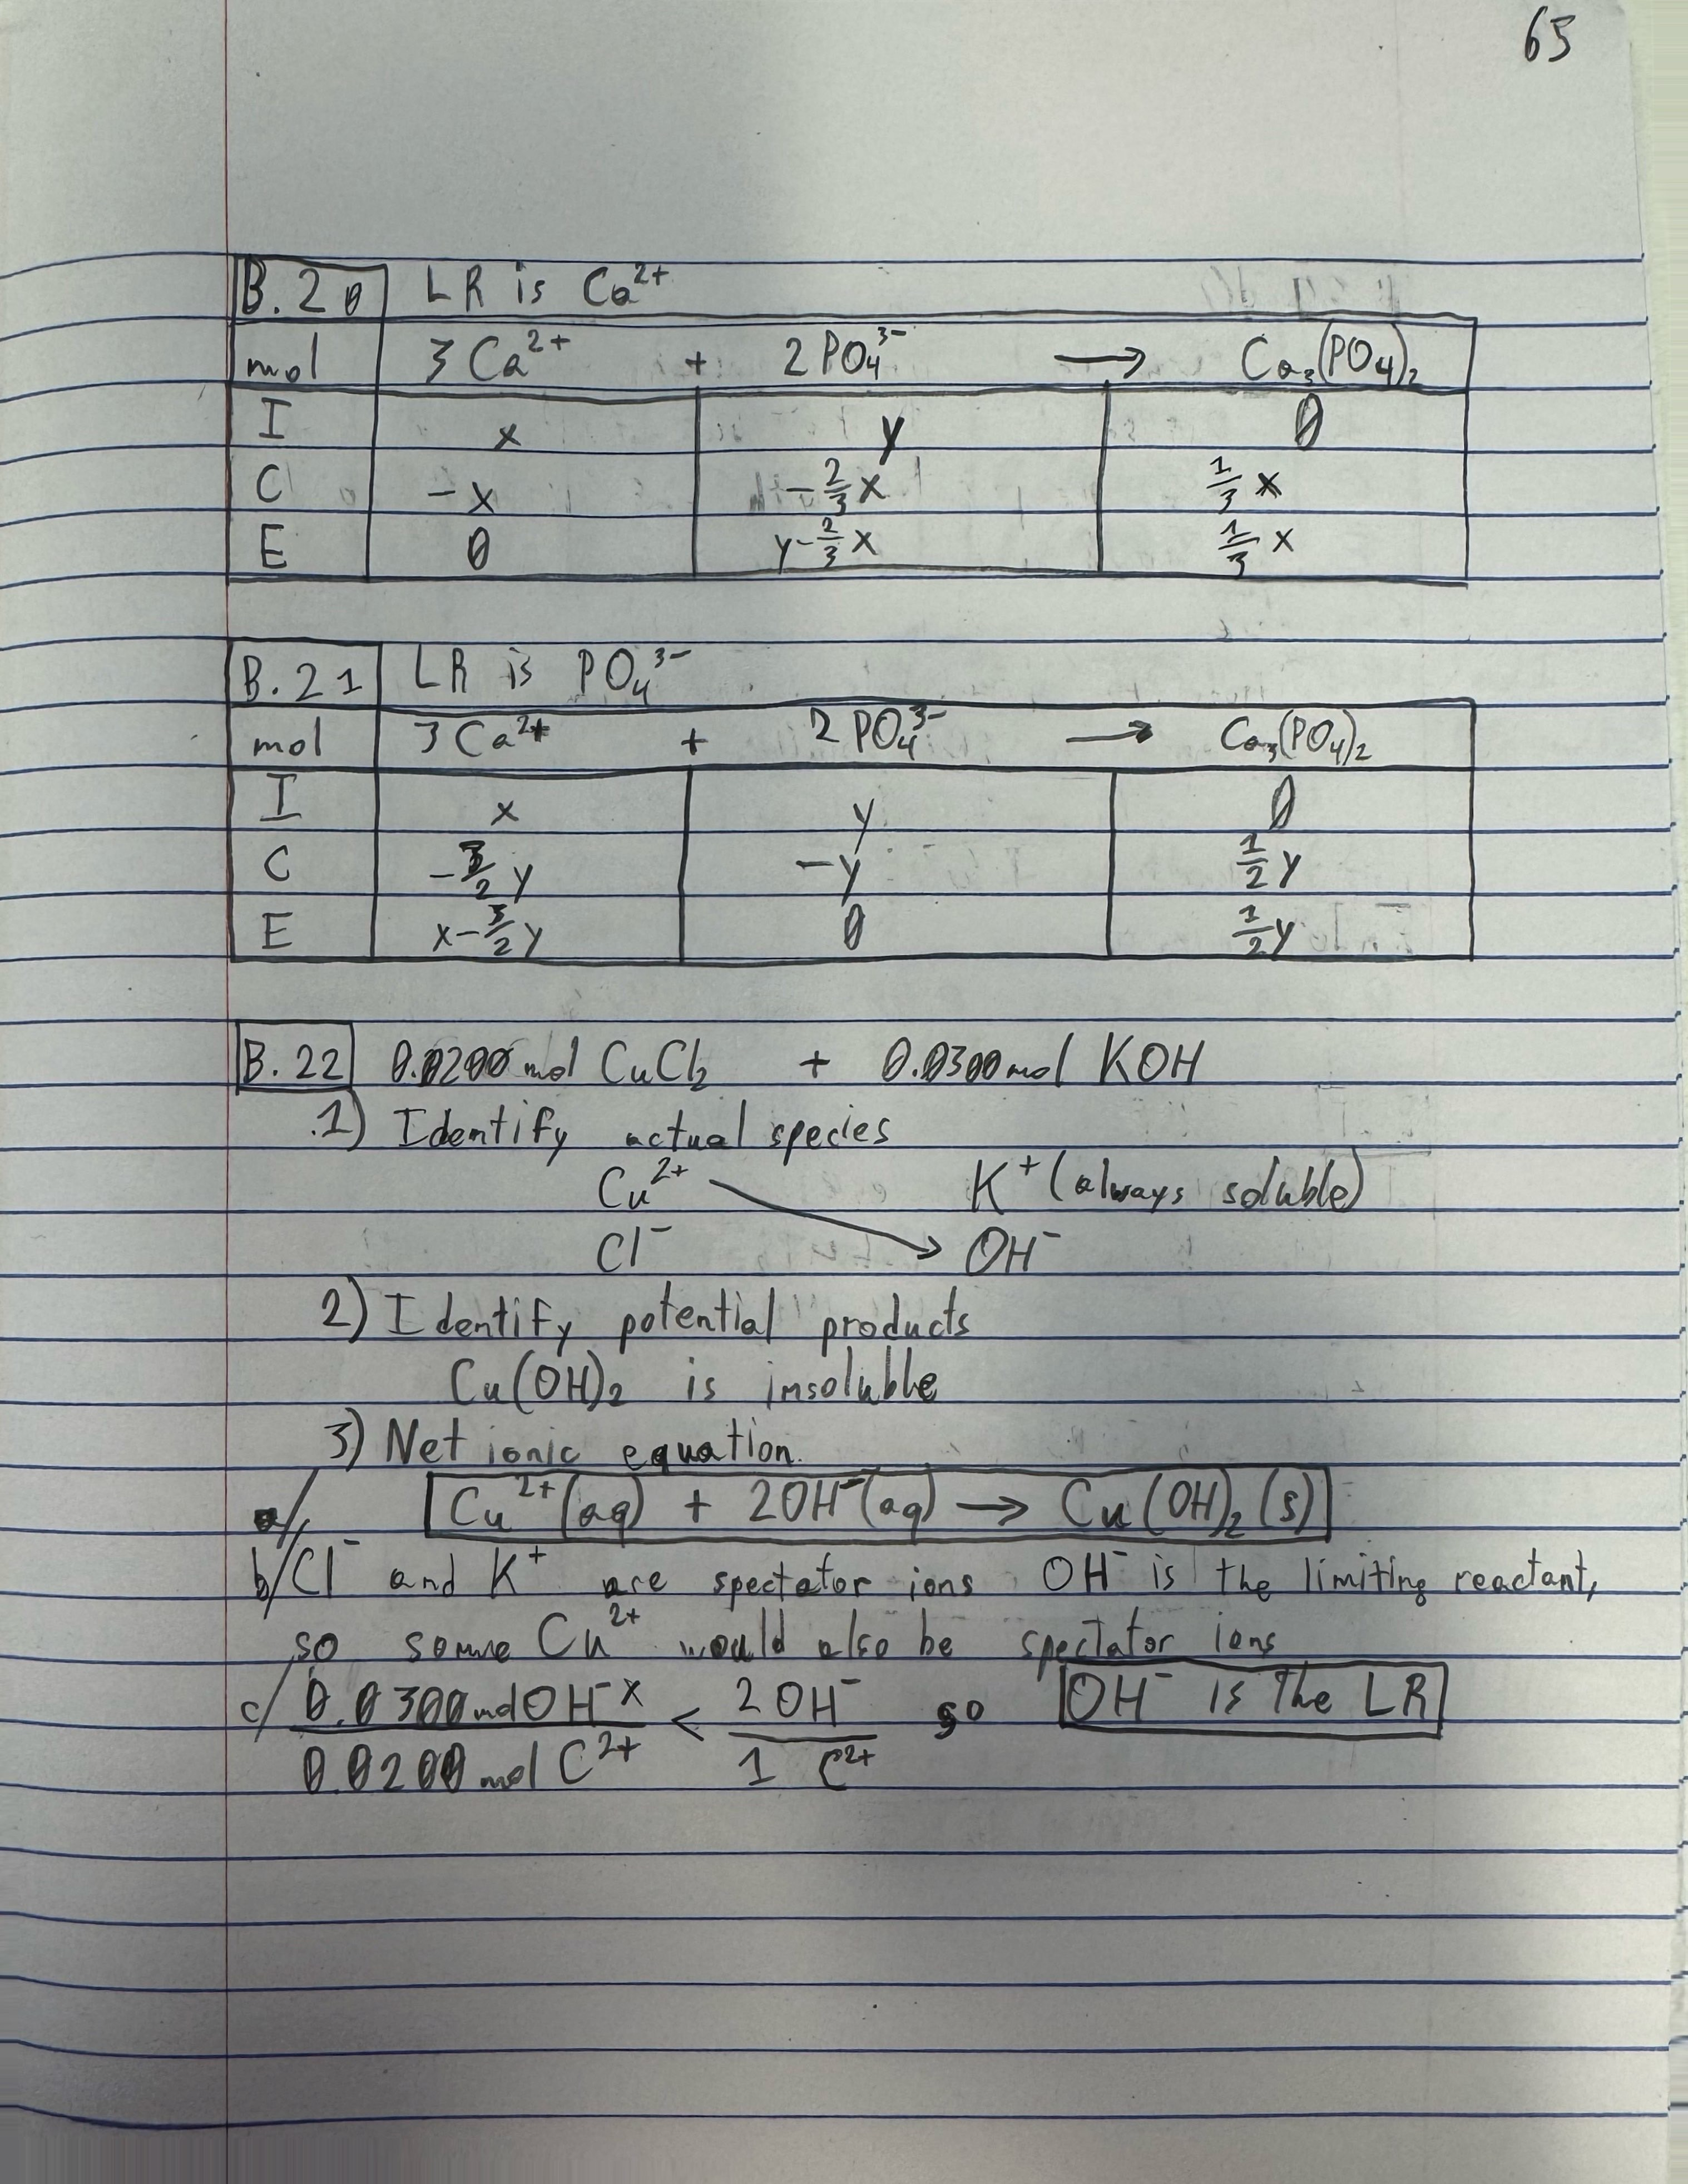
\includegraphics[width=\textwidth, trim={5in 9in 1in 25in},clip]{"Answers Images/IMG_6651.jpg"}

                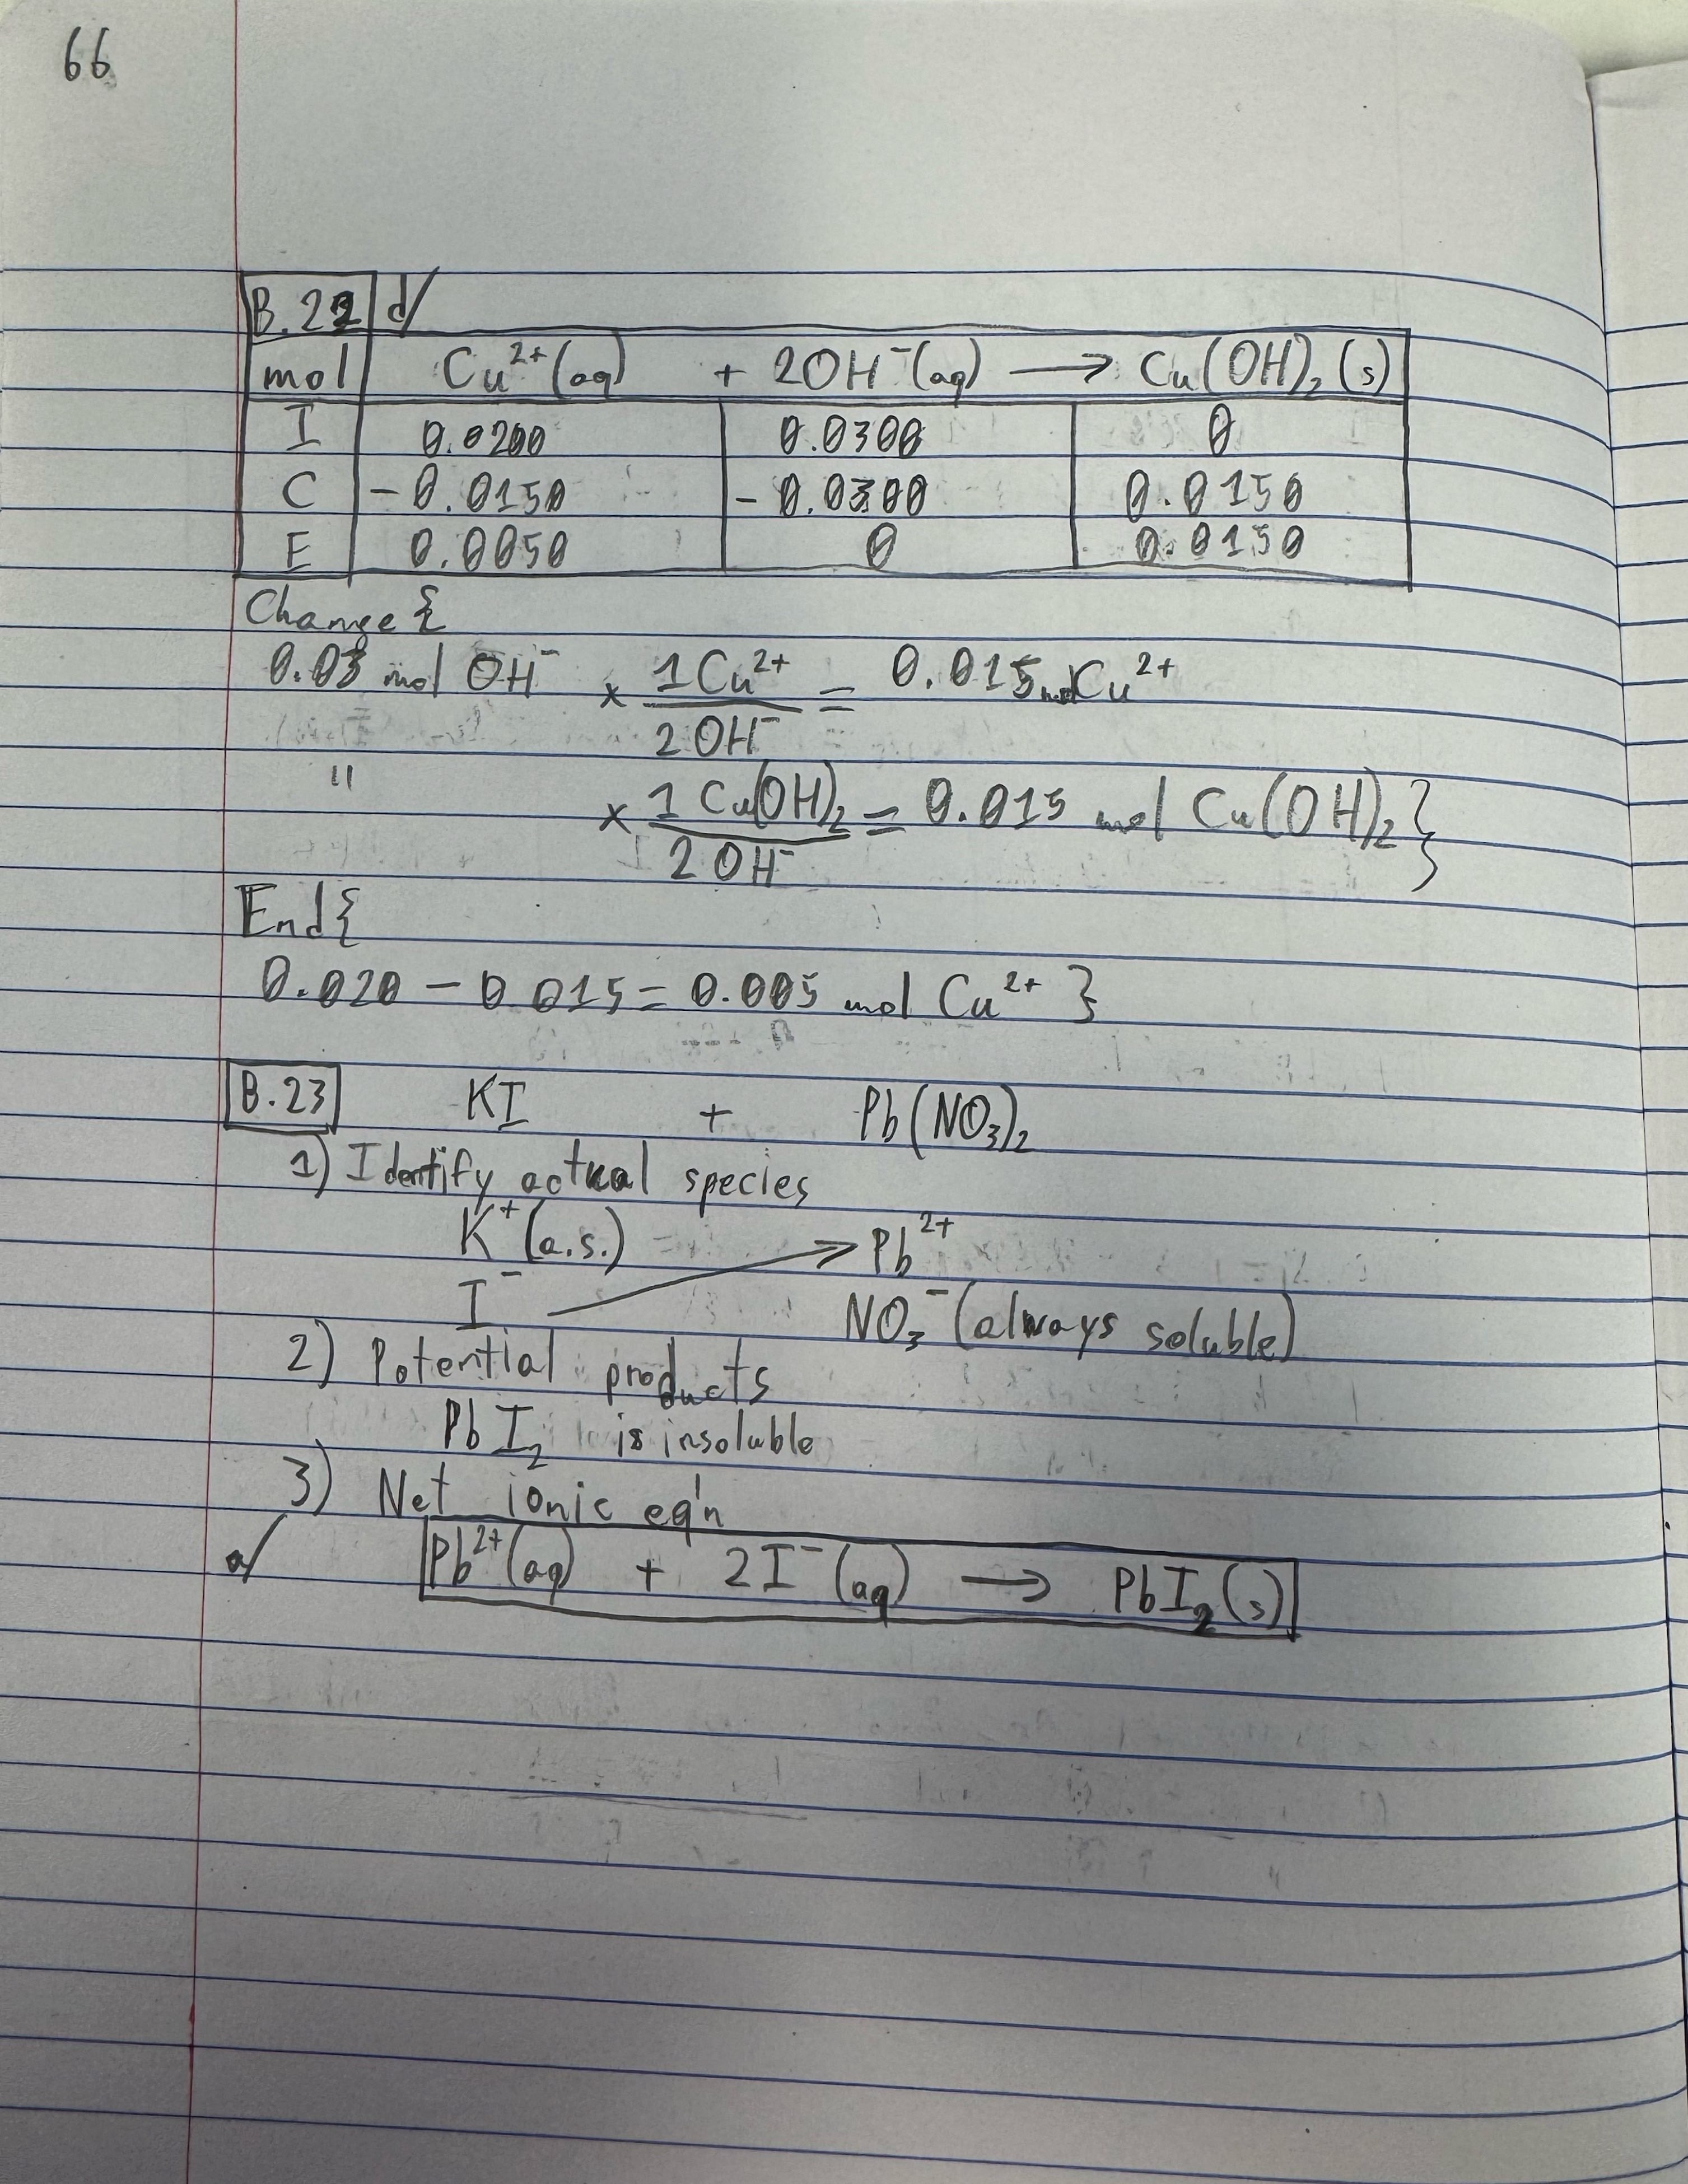
\includegraphics[width=\textwidth, trim={5in 27in 3in 7in},clip]{"Answers Images/IMG_6652.jpg"}
            \end{center}

    \pagebreak
    \section{Topic B Problem 23}
        A chemist mixes 5.00 mL of 0.240 M \ce{KI} with 4.00 mL of 0.200 M \ce{Pb(NO3)2}.
        
        a) Write the balanced net ionic equation for the reaction that occurs.
        
        b) Construct an ICE table for this reaction, using the net ionic equation.
        
        c) What mass of solid product is formed?
        
        d) What is the concentration of the excess reactant in the final mixture?
        
        e) What is the concentration of nitrate ions in the final mixture?

        \subsection{Solution}
            \begin{center}
                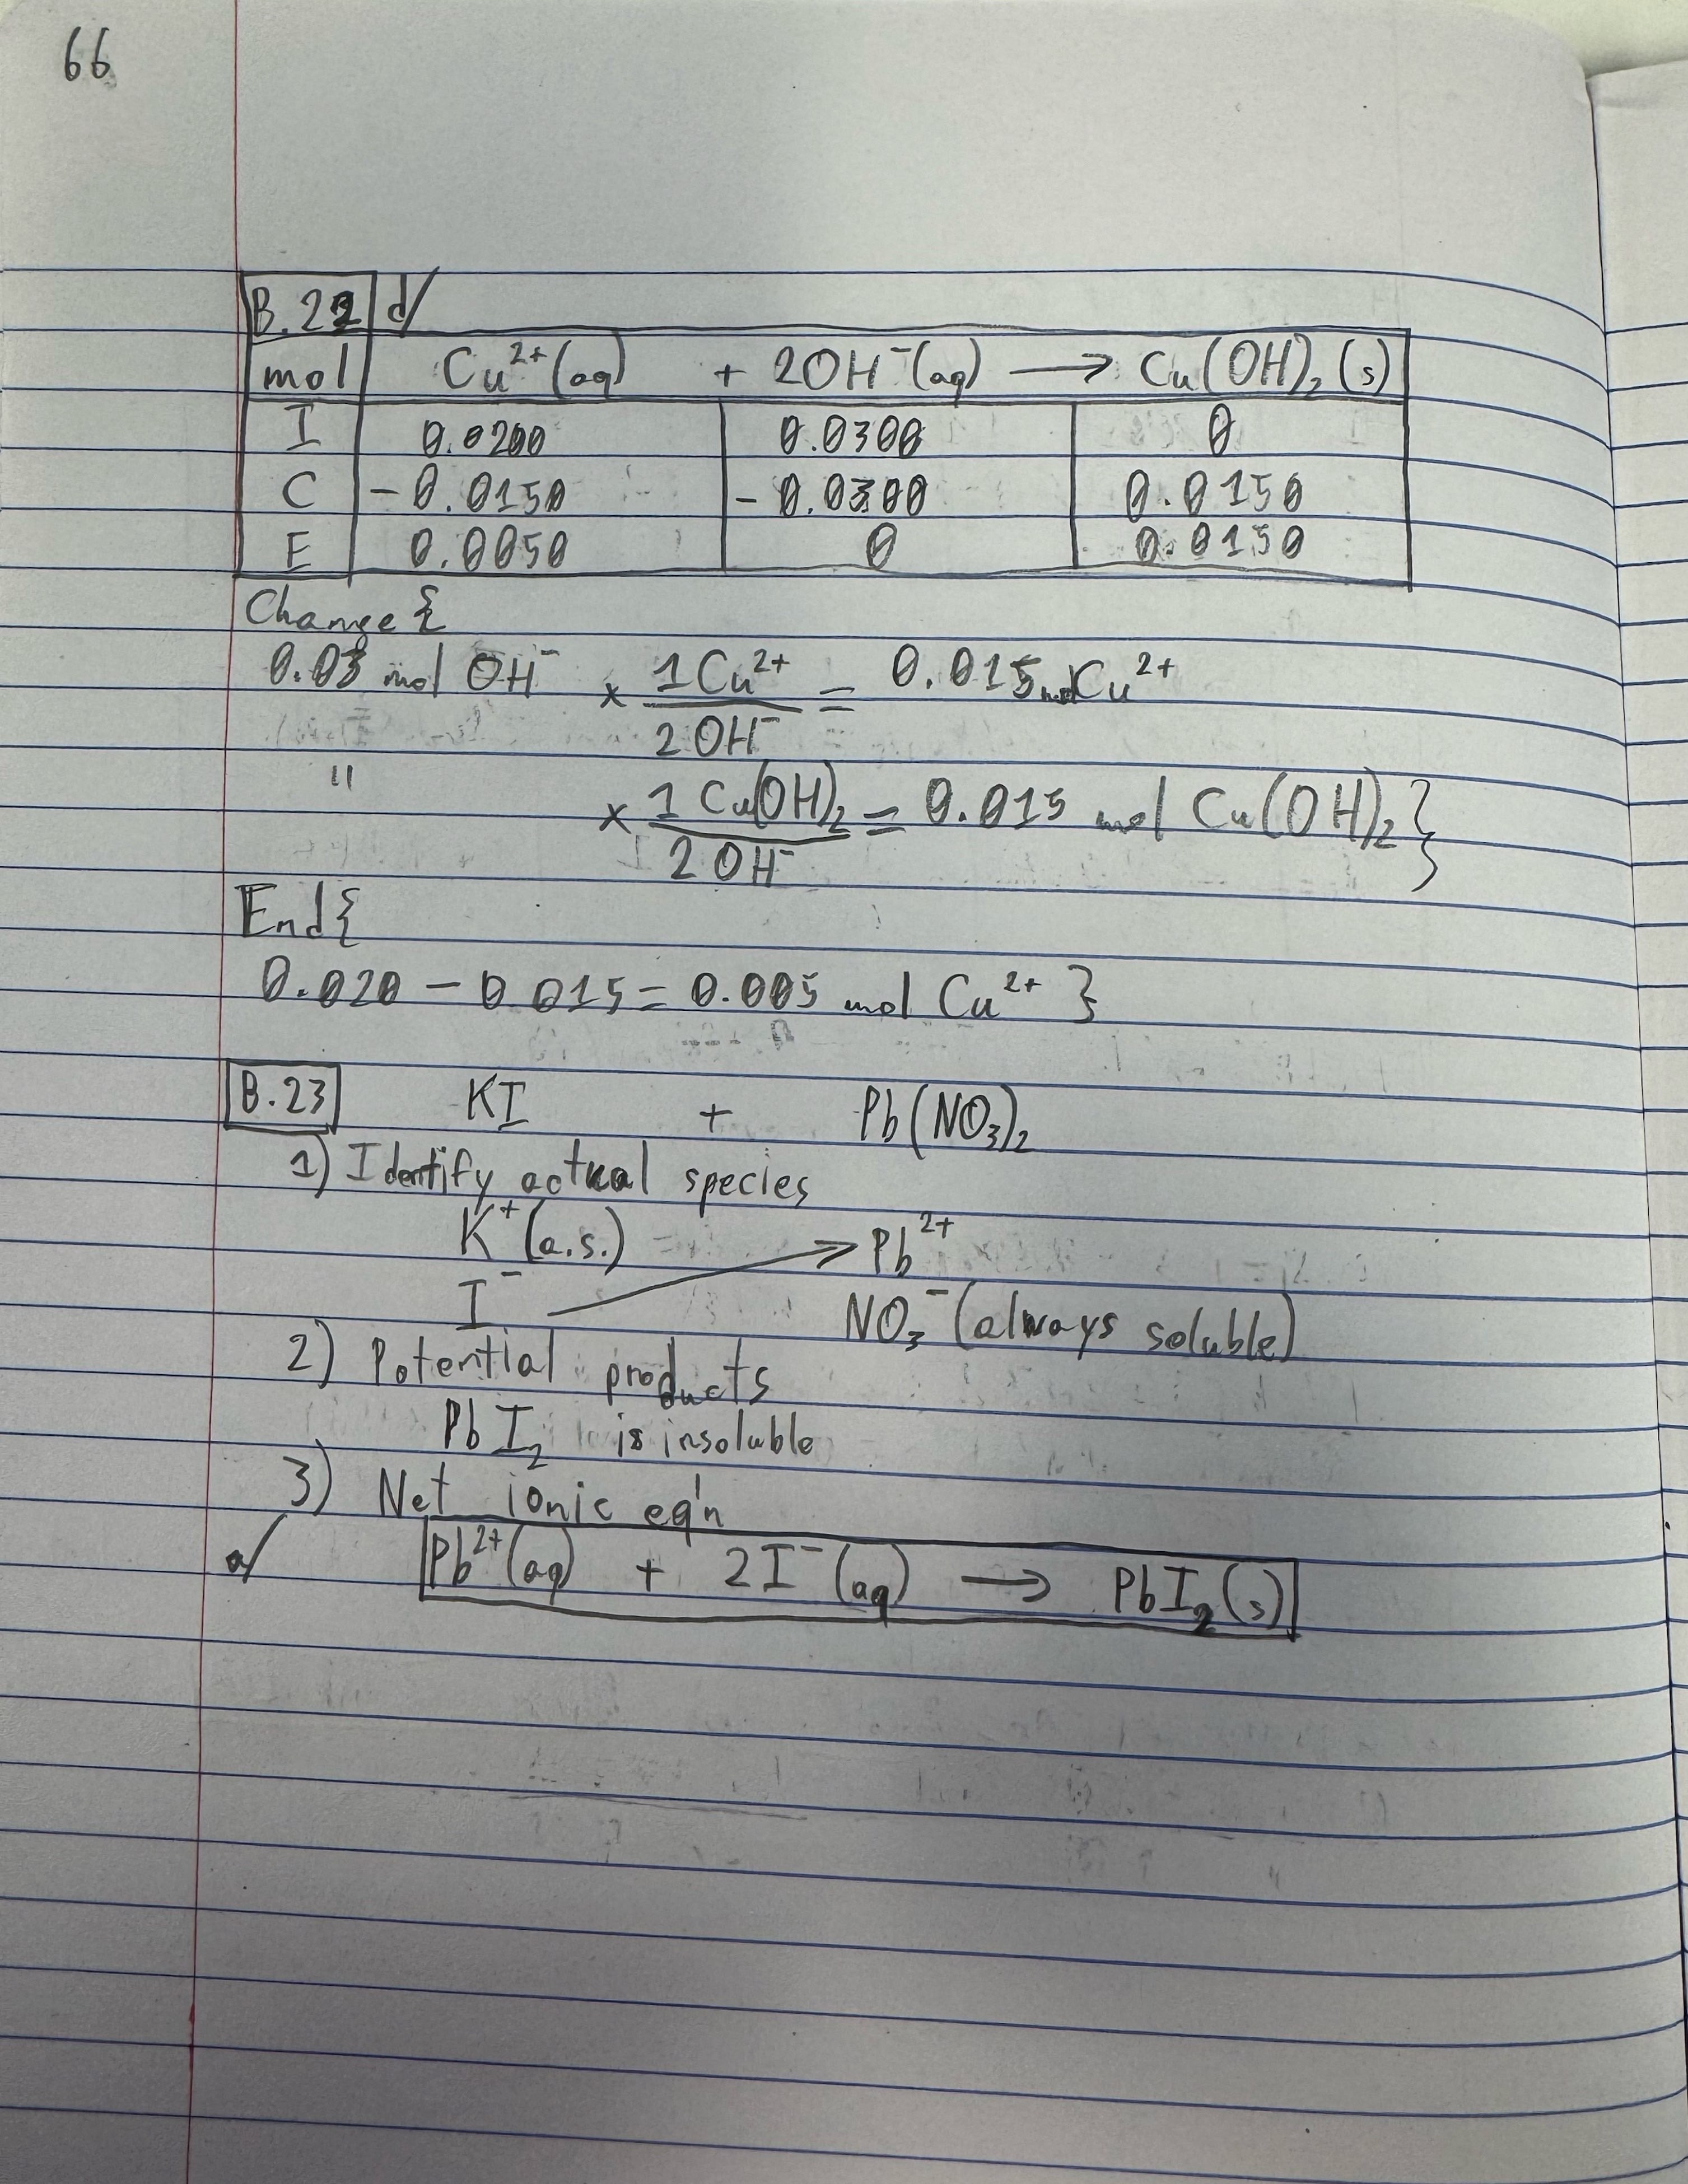
\includegraphics[width=\textwidth, trim={5in 13in 3in 26in},clip]{"Answers Images/IMG_6652.jpg"}
                
                Continued on next page

                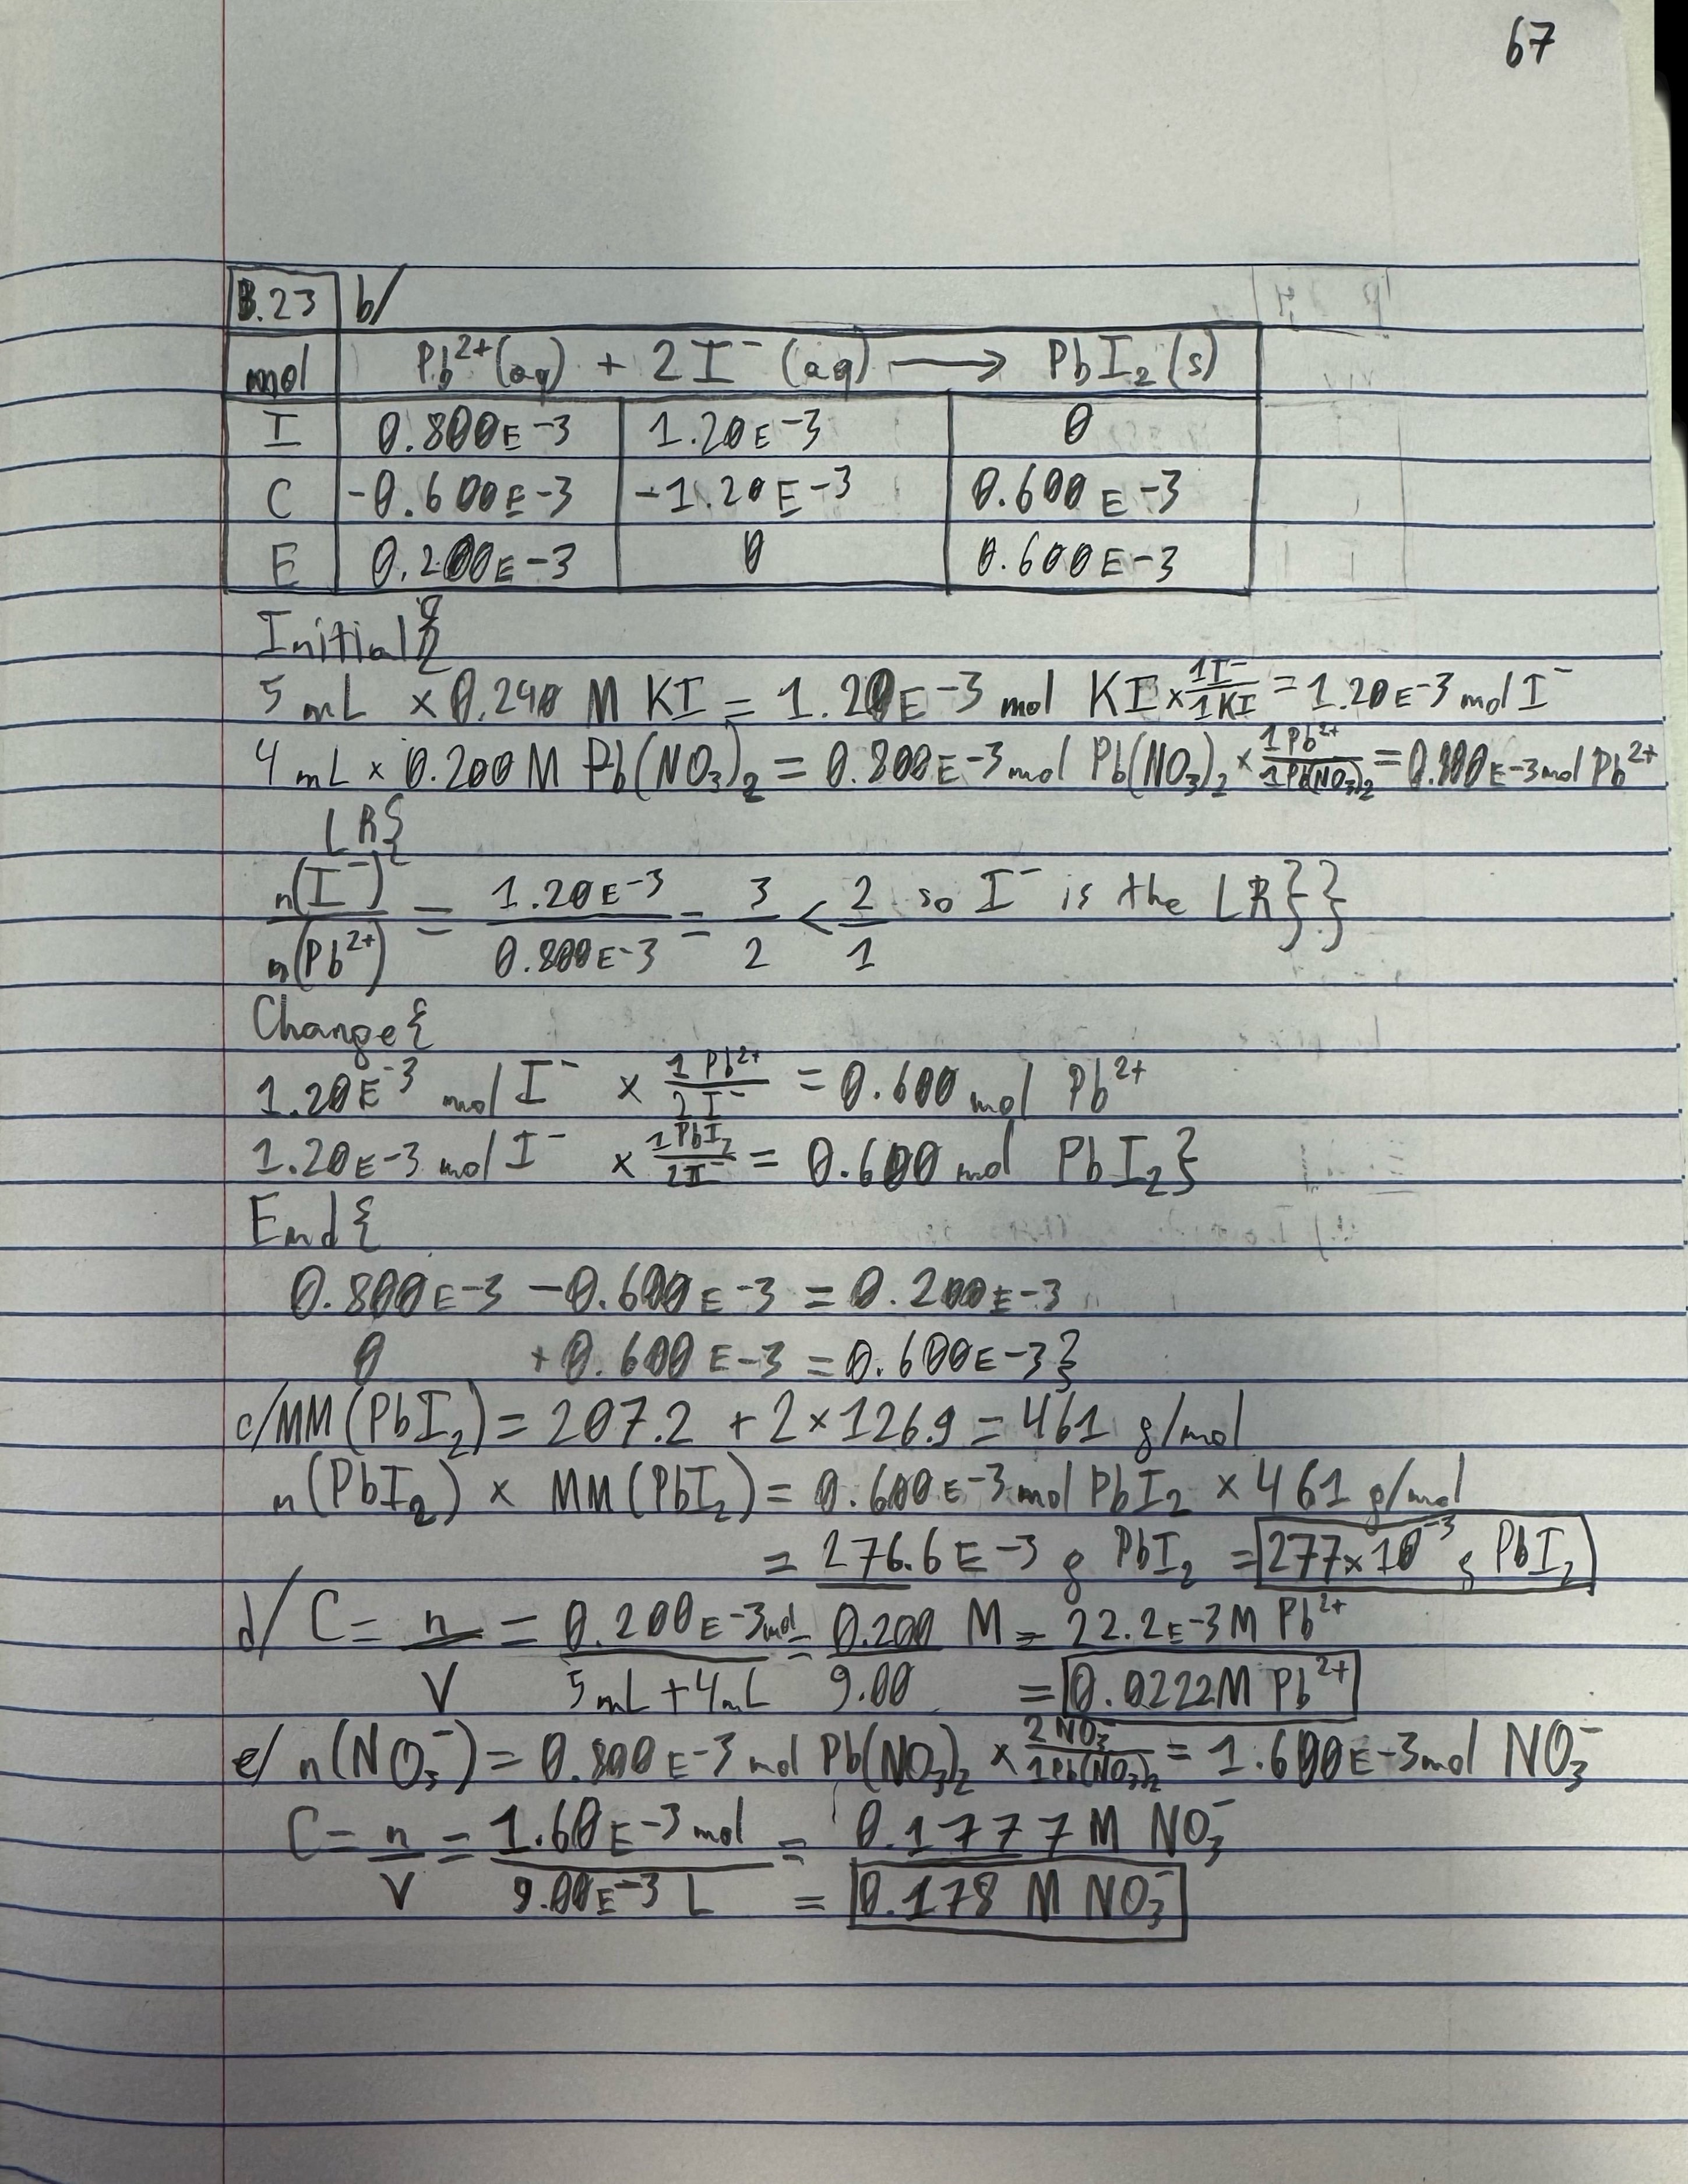
\includegraphics[width=\textwidth, trim={5in 2in 0in 6in},clip]{"Answers Images/IMG_6653.jpg"}
            \end{center}

    \pagebreak
    \section{Topic B Problem 24}
        A chemist adds 1.35 g of solid \ce{Ag2O} to 25.0 mL of 2.00 M \ce{HBr}, causing this reaction:
        \begin{center}
            \ce{Ag2O(s) + 2 H+(aq) + 2 Br-(aq) -> 2 AgBr(s) + H2O(l)}
        \end{center}
        
        a) What mass of solid \ce{AgBr} is formed?
        
        b) What is the concentration of H+ ions in the final mixture? 
        (You may assume that the final solution volume is 25.0 mL.)

        \subsection{Solution}
            \begin{center}
                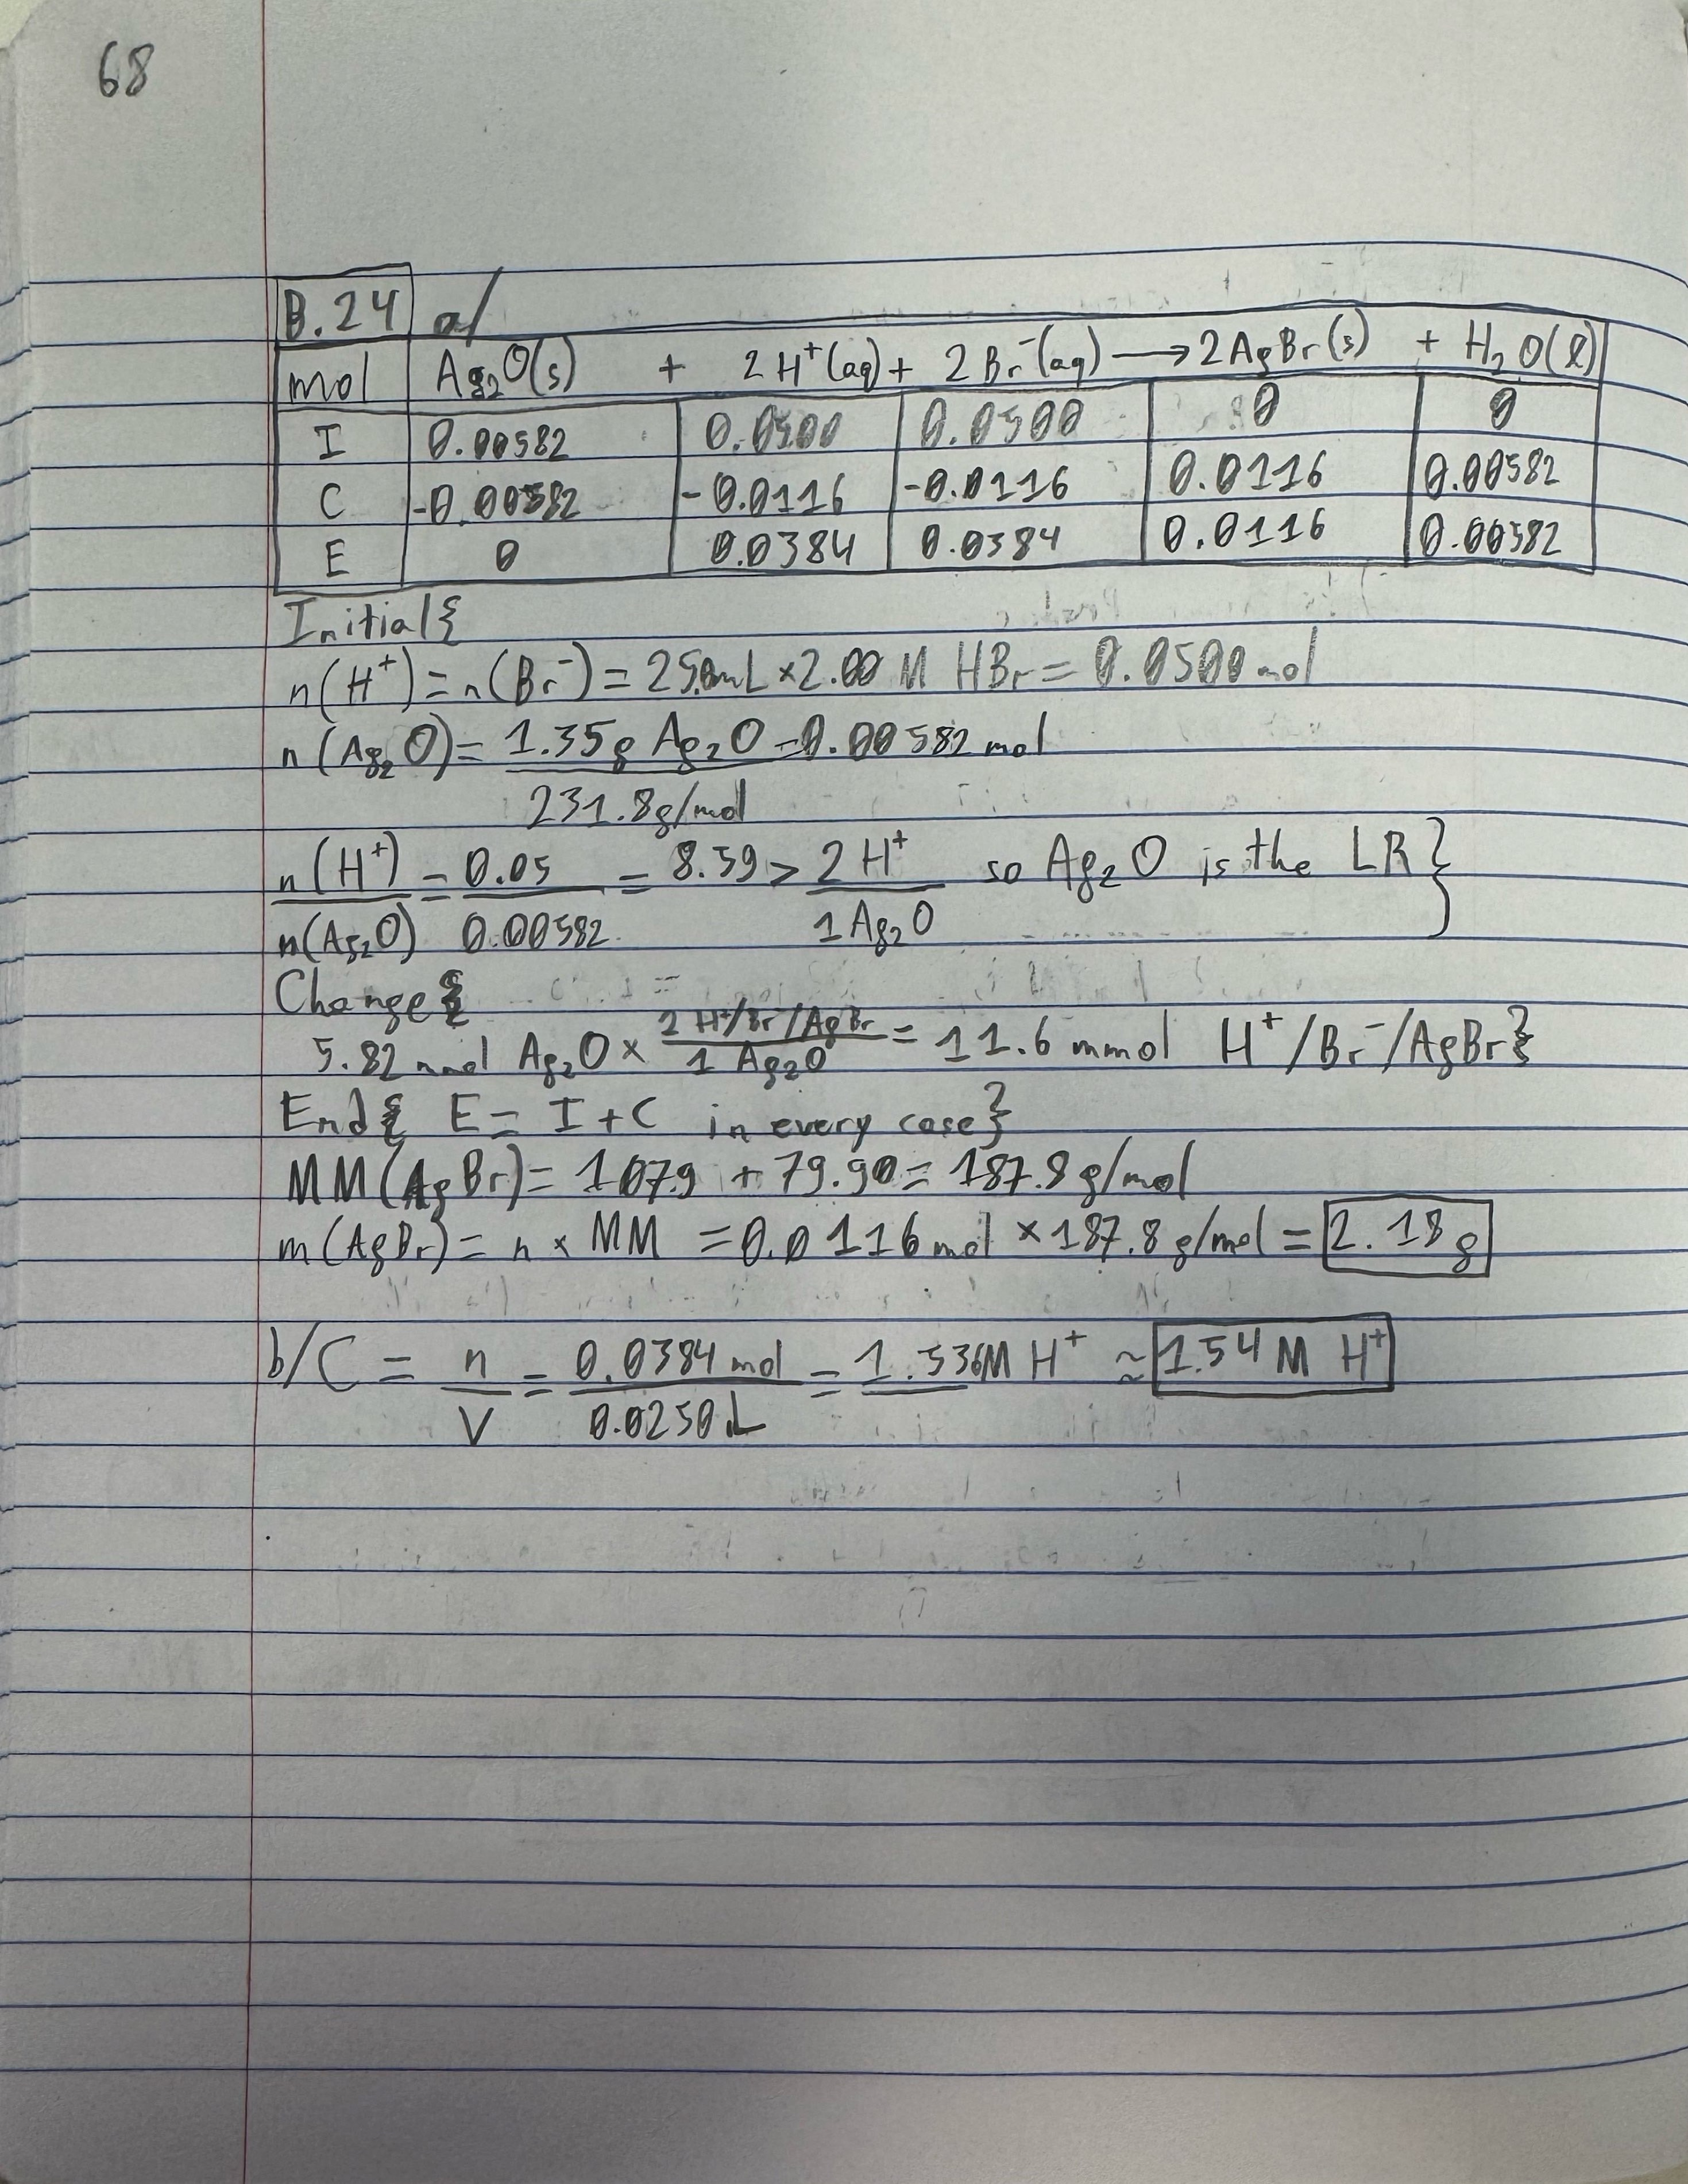
\includegraphics[width=\textwidth, trim={5in 15in 1in 6in},clip]{"Answers Images/IMG_6654.jpg"}
            \end{center}

    \pagebreak
    \section{Topic B Problem 25}
        You have 50.0 mL of a 0.138 M \ce{Ba(NO3)2} solution. 
        What is the minimum volume of 0.131 M \ce{Na3PO4} solution that you must add in order to remove all of the barium ions from the solution?

        \subsection{Solution}
            \begin{center}
                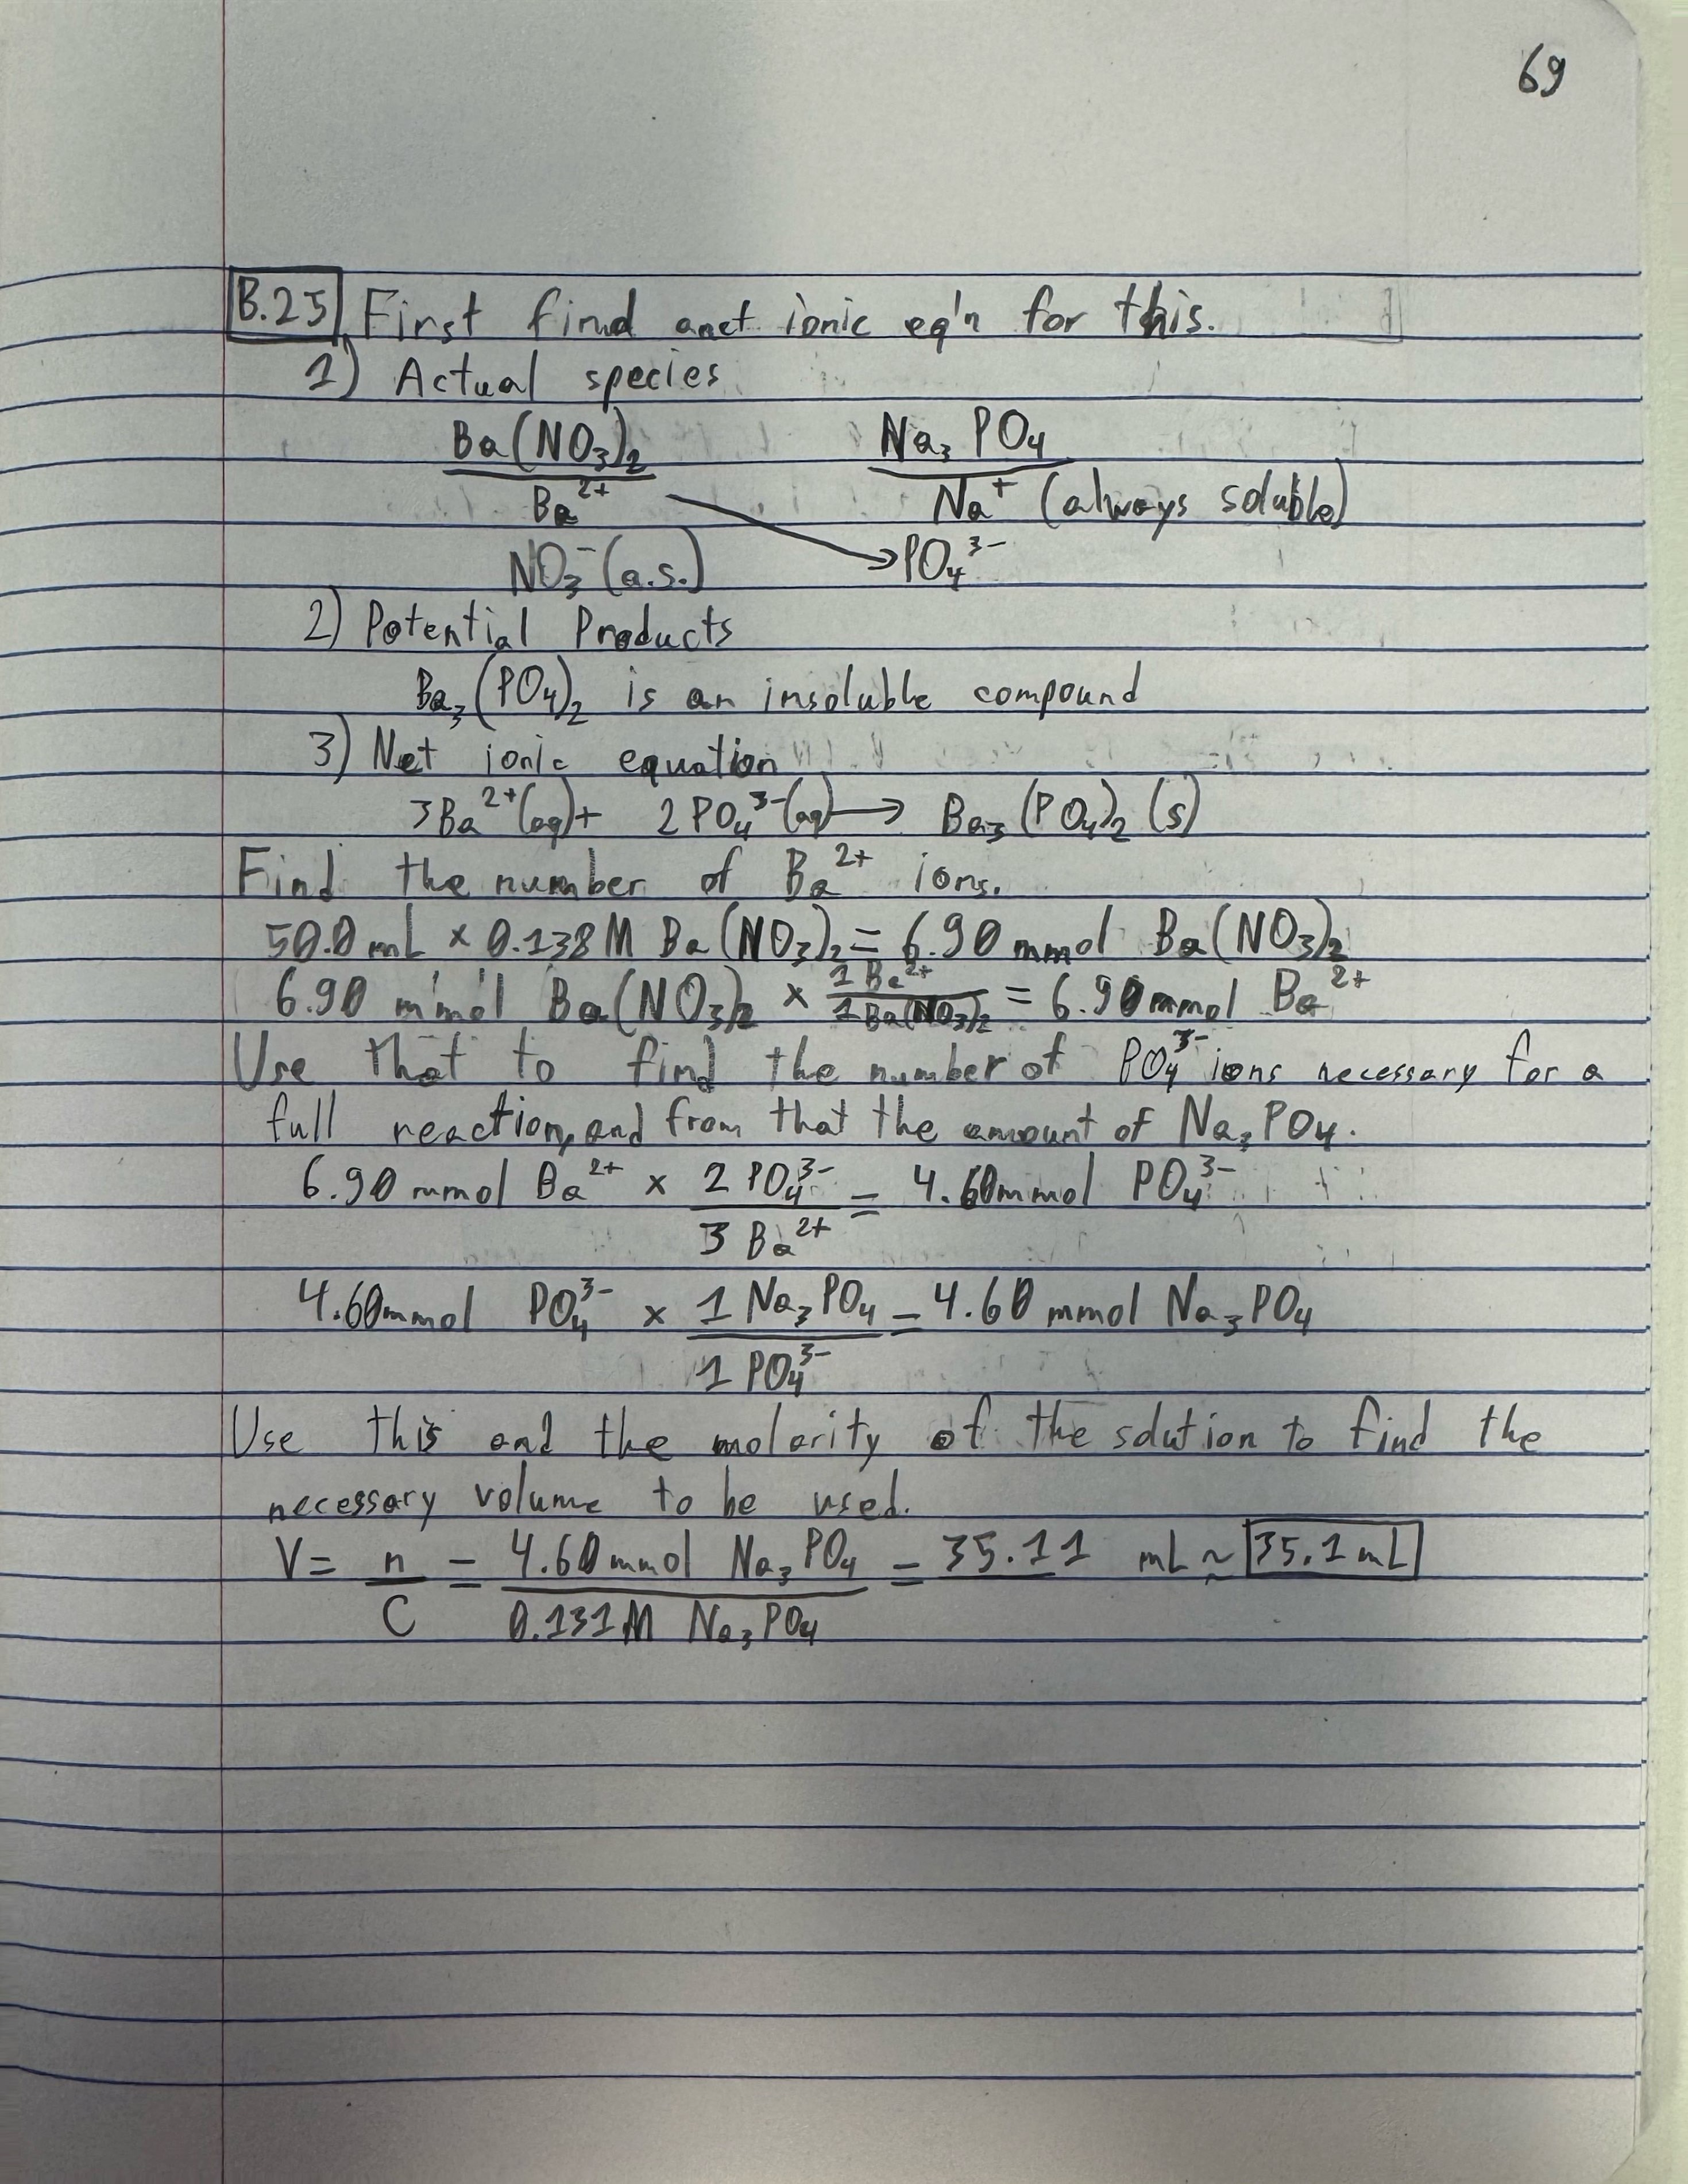
\includegraphics[width=\textwidth, trim={5in 10in 3in 6in},clip]{"Answers Images/IMG_6655.jpg"}
            \end{center}

    \pagebreak
    \section{Topic B Problem 26}
        A solution contains an unknown concentration of sulfate ions. When 20.00 mL of this solution is mixed with excess aqueous \ce{Ba(NO3)2}, 0.877 g of \ce{BaSO4} is formed. 
        Calculate the molarity of sulfate ions in the original solution.

        \subsection{Solution}
            \begin{center}
                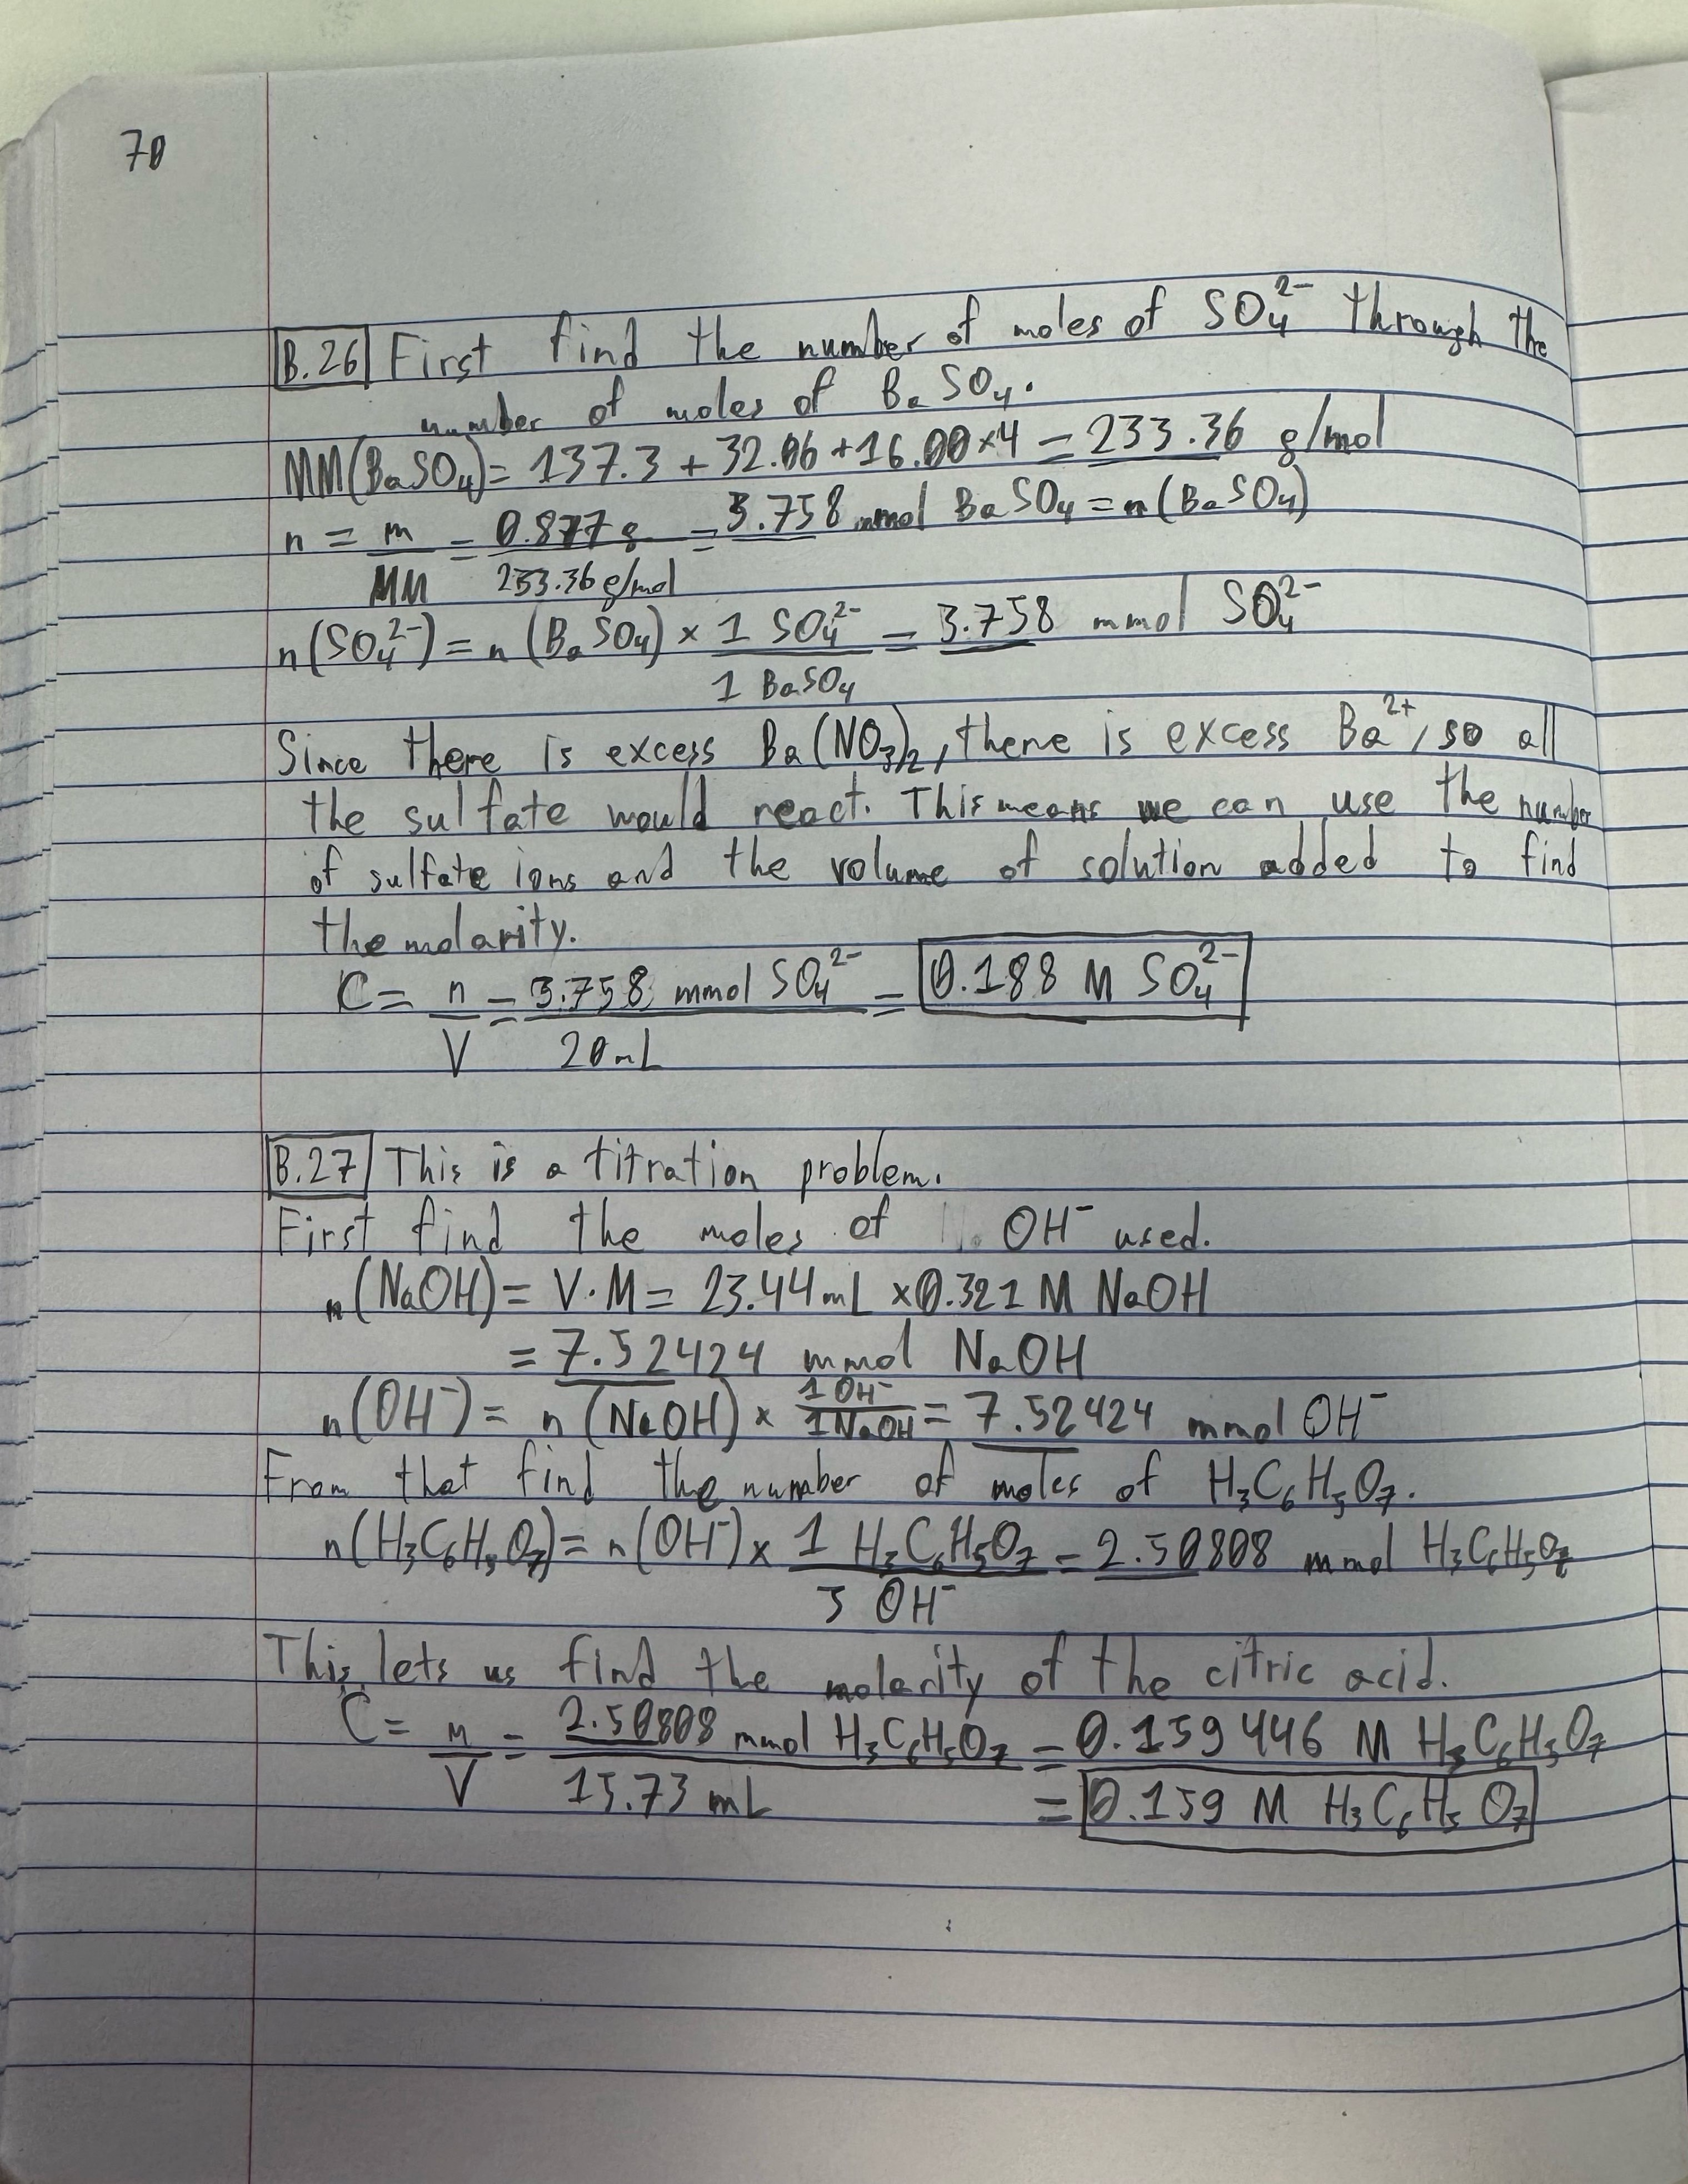
\includegraphics[width=\textwidth, trim={5in 27in 1in 6in},clip]{"Answers Images/IMG_6656.jpg"}
            \end{center}

    \pagebreak
    \section{Topic B Problem 27}
        A solution contains an unknown concentration of citric acid, \ce{H3C6H5O7}. 
        A 15.73 mL portion of this solution is placed in a flask and titrated with 0.321 M \ce{NaOH}. 
        The endpoint is reached when 23.44 mL of the NaOH solution has been added. 
        Calculate the molarity of the original citric acid solution. 
        The net ionic equation for the reaction that occurs is:
        \begin{center}
            \ce{3 OH-(aq) + H3C6H5O7(aq) -> 3 H2O(l) + C6H5O7^3-(aq)}
        \end{center}

        \subsection{Solution}
            \begin{center}
                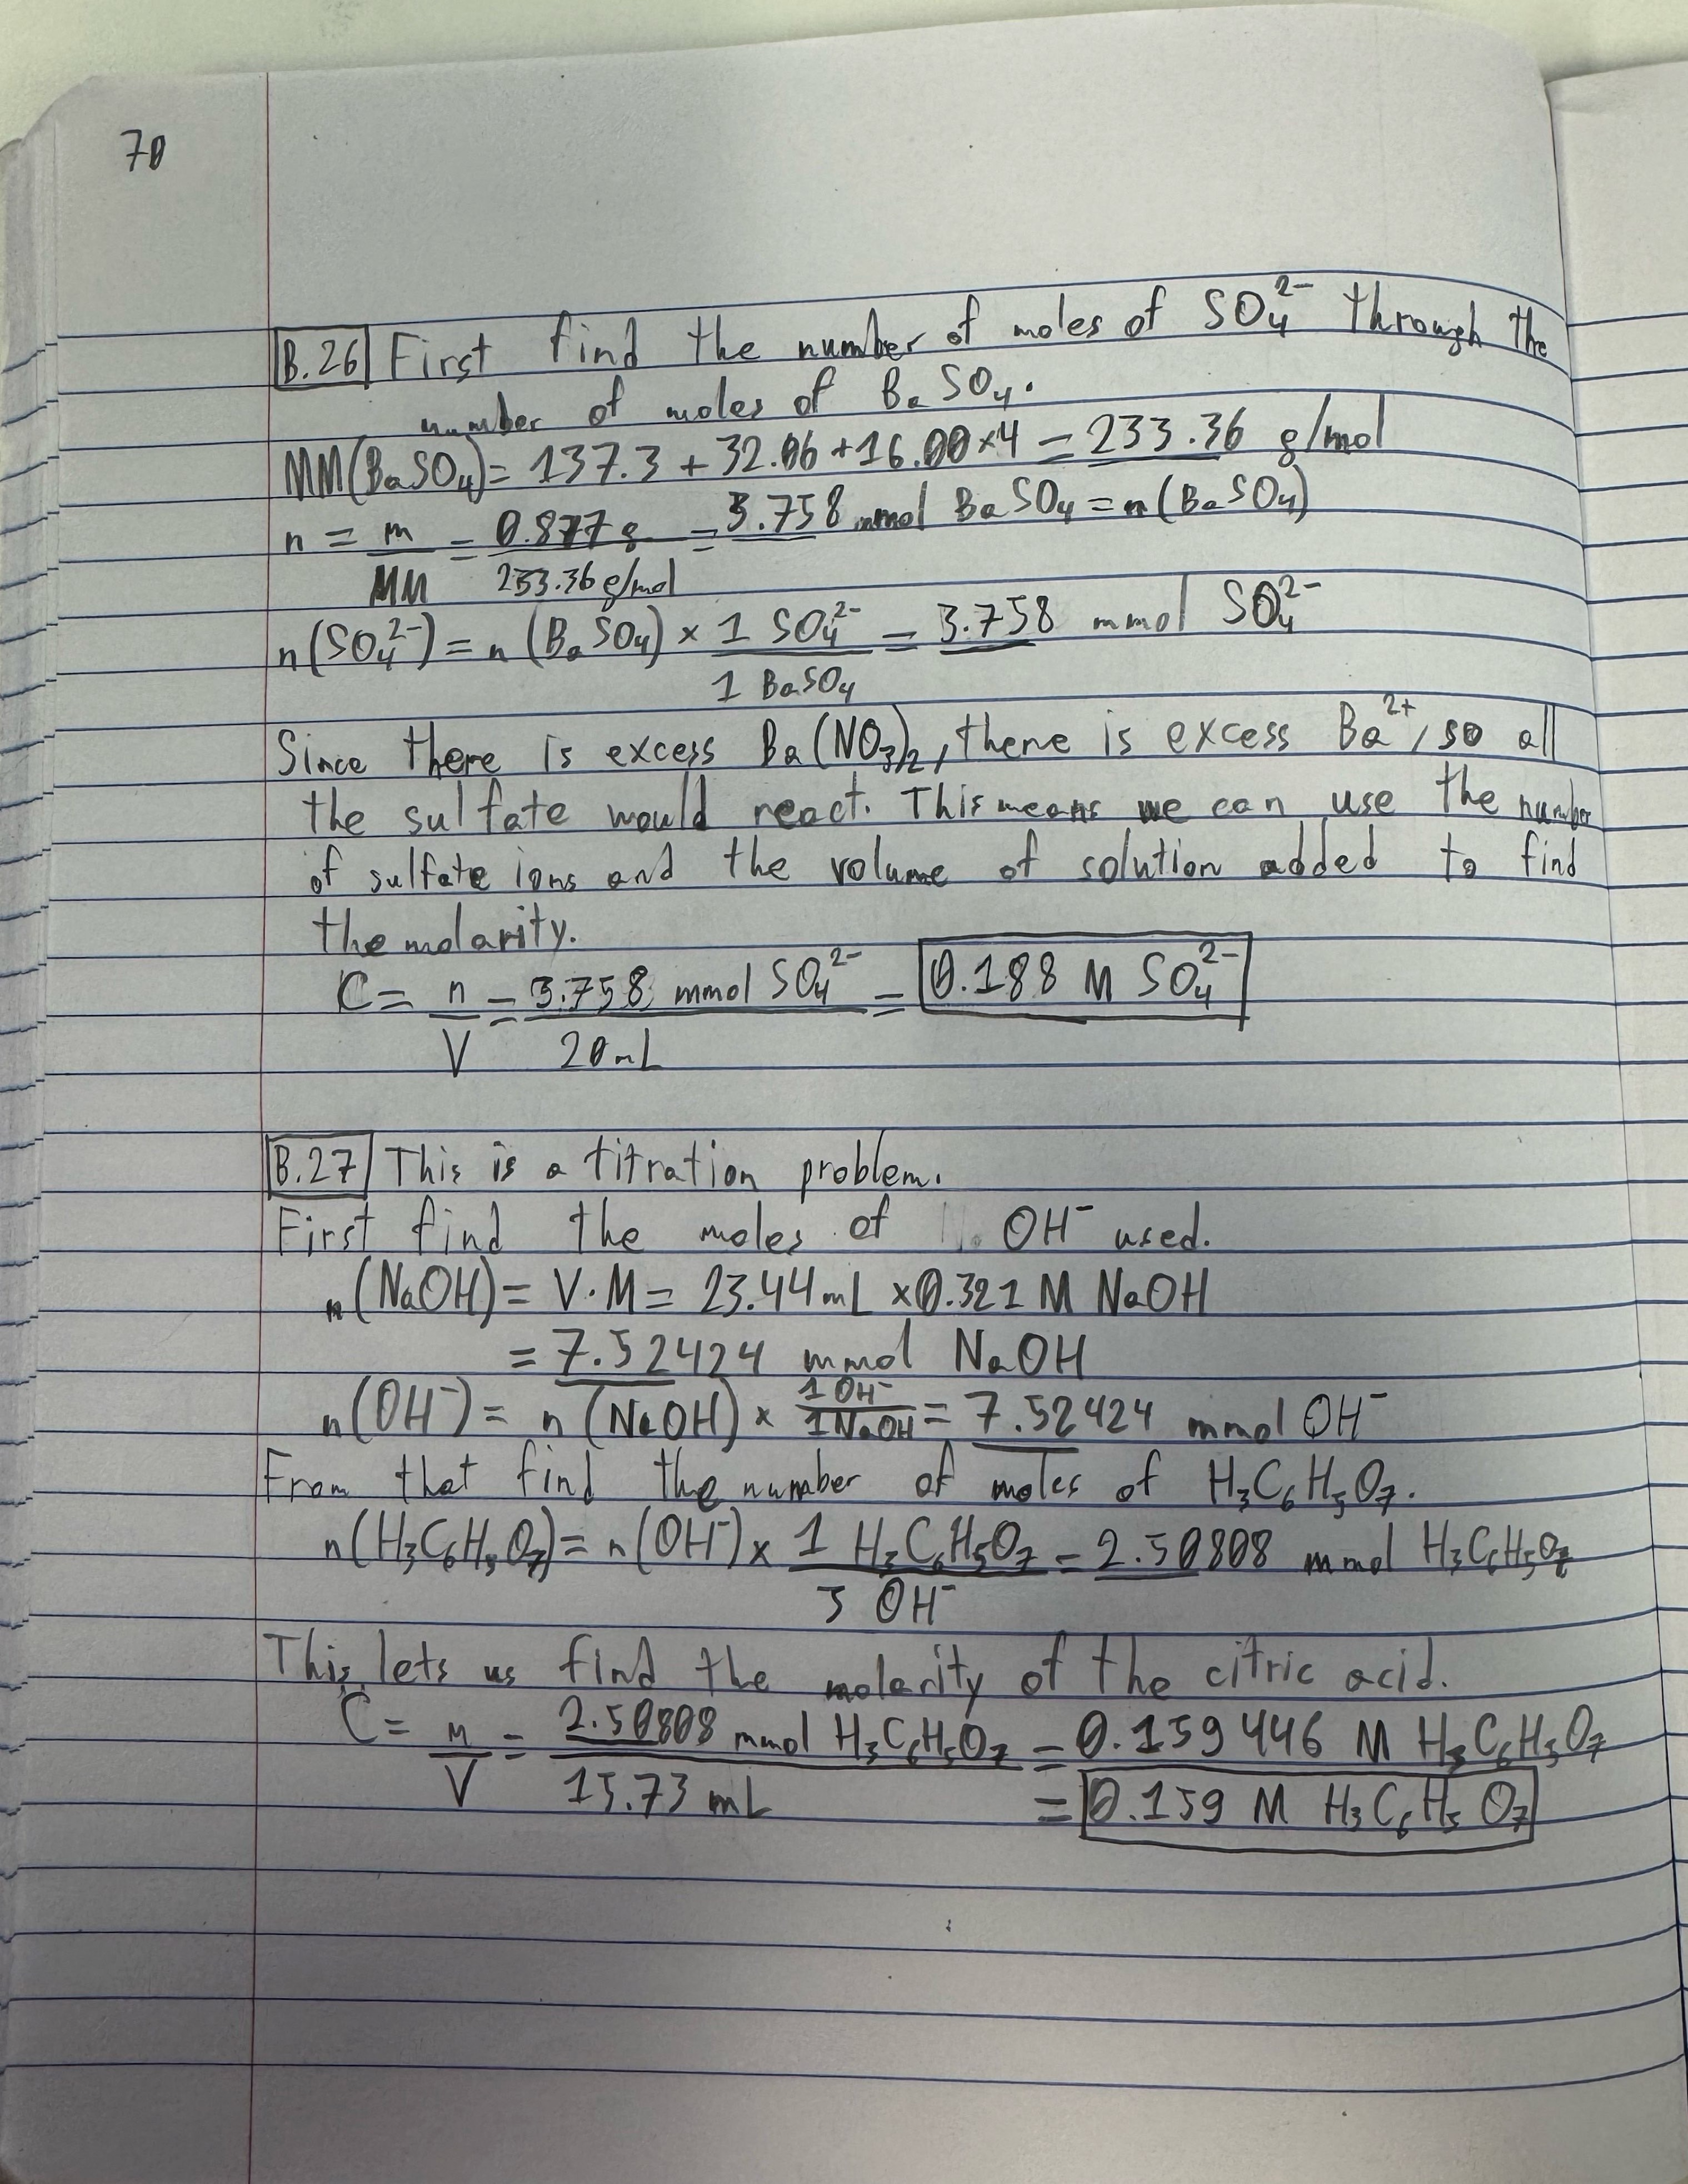
\includegraphics[width=\textwidth, trim={5in 7in 1in 28in},clip]{"Answers Images/IMG_6656.jpg"}
            \end{center}

    \pagebreak

    \tableofcontents
\end{document}